% Options for packages loaded elsewhere
\PassOptionsToPackage{unicode}{hyperref}
\PassOptionsToPackage{hyphens}{url}
\PassOptionsToPackage{dvipsnames,svgnames,x11names}{xcolor}
%
\documentclass[
  12pt,
]{article}
\usepackage{amsmath,amssymb}
\usepackage{iftex}
\ifPDFTeX
  \usepackage[T1]{fontenc}
  \usepackage[utf8]{inputenc}
  \usepackage{textcomp} % provide euro and other symbols
\else % if luatex or xetex
  \usepackage{unicode-math} % this also loads fontspec
  \defaultfontfeatures{Scale=MatchLowercase}
  \defaultfontfeatures[\rmfamily]{Ligatures=TeX,Scale=1}
\fi
\usepackage{lmodern}
\ifPDFTeX\else
  % xetex/luatex font selection
\fi
% Use upquote if available, for straight quotes in verbatim environments
\IfFileExists{upquote.sty}{\usepackage{upquote}}{}
\IfFileExists{microtype.sty}{% use microtype if available
  \usepackage[]{microtype}
  \UseMicrotypeSet[protrusion]{basicmath} % disable protrusion for tt fonts
}{}
\makeatletter
\@ifundefined{KOMAClassName}{% if non-KOMA class
  \IfFileExists{parskip.sty}{%
    \usepackage{parskip}
  }{% else
    \setlength{\parindent}{0pt}
    \setlength{\parskip}{6pt plus 2pt minus 1pt}}
}{% if KOMA class
  \KOMAoptions{parskip=half}}
\makeatother
\usepackage{xcolor}
\usepackage[margin=1in]{geometry}
\usepackage{longtable,booktabs,array}
\usepackage{calc} % for calculating minipage widths
% Correct order of tables after \paragraph or \subparagraph
\usepackage{etoolbox}
\makeatletter
\patchcmd\longtable{\par}{\if@noskipsec\mbox{}\fi\par}{}{}
\makeatother
% Allow footnotes in longtable head/foot
\IfFileExists{footnotehyper.sty}{\usepackage{footnotehyper}}{\usepackage{footnote}}
\makesavenoteenv{longtable}
\usepackage{graphicx}
\makeatletter
\def\maxwidth{\ifdim\Gin@nat@width>\linewidth\linewidth\else\Gin@nat@width\fi}
\def\maxheight{\ifdim\Gin@nat@height>\textheight\textheight\else\Gin@nat@height\fi}
\makeatother
% Scale images if necessary, so that they will not overflow the page
% margins by default, and it is still possible to overwrite the defaults
% using explicit options in \includegraphics[width, height, ...]{}
\setkeys{Gin}{width=\maxwidth,height=\maxheight,keepaspectratio}
% Set default figure placement to htbp
\makeatletter
\def\fps@figure{htbp}
\makeatother
\setlength{\emergencystretch}{3em} % prevent overfull lines
\providecommand{\tightlist}{%
  \setlength{\itemsep}{0pt}\setlength{\parskip}{0pt}}
\setcounter{secnumdepth}{5}
\newlength{\cslhangindent}
\setlength{\cslhangindent}{1.5em}
\newlength{\csllabelwidth}
\setlength{\csllabelwidth}{3em}
\newlength{\cslentryspacingunit} % times entry-spacing
\setlength{\cslentryspacingunit}{\parskip}
\newenvironment{CSLReferences}[2] % #1 hanging-ident, #2 entry spacing
 {% don't indent paragraphs
  \setlength{\parindent}{0pt}
  % turn on hanging indent if param 1 is 1
  \ifodd #1
  \let\oldpar\par
  \def\par{\hangindent=\cslhangindent\oldpar}
  \fi
  % set entry spacing
  \setlength{\parskip}{#2\cslentryspacingunit}
 }%
 {}
\usepackage{calc}
\newcommand{\CSLBlock}[1]{#1\hfill\break}
\newcommand{\CSLLeftMargin}[1]{\parbox[t]{\csllabelwidth}{#1}}
\newcommand{\CSLRightInline}[1]{\parbox[t]{\linewidth - \csllabelwidth}{#1}\break}
\newcommand{\CSLIndent}[1]{\hspace{\cslhangindent}#1}
\usepackage{floatrow}
\floatsetup{capposition=top}
\usepackage{setspace}
\usepackage{fancyhdr}
\usepackage{titlesec}
\usepackage{geometry}
\usepackage{subfig}
\newcommand{\beginsupplement}{
\setcounter{table}{0}
\renewcommand{\thetable}{S\arabic{table}}
\setcounter{figure}{0}
\renewcommand{\thefigure}{S\arabic{figure}}}
\usepackage{booktabs}
\usepackage{longtable}
\usepackage{array}
\usepackage{multirow}
\usepackage{wrapfig}
\usepackage{float}
\usepackage{colortbl}
\usepackage{pdflscape}
\usepackage{tabu}
\usepackage{threeparttable}
\usepackage{threeparttablex}
\usepackage[normalem]{ulem}
\usepackage{makecell}
\usepackage{xcolor}
\ifLuaTeX
  \usepackage{selnolig}  % disable illegal ligatures
\fi
\IfFileExists{bookmark.sty}{\usepackage{bookmark}}{\usepackage{hyperref}}
\IfFileExists{xurl.sty}{\usepackage{xurl}}{} % add URL line breaks if available
\urlstyle{same}
\hypersetup{
  pdftitle={A Sociological Analysis of Structural Racism in `Student List' Lead Generation Products},
  pdfauthor={Ozan Jaquette; Karina G. Salazar},
  colorlinks=true,
  linkcolor={Maroon},
  filecolor={Maroon},
  citecolor={Blue},
  urlcolor={blue},
  pdfcreator={LaTeX via pandoc}}

\title{A Sociological Analysis of Structural Racism in `Student List' Lead Generation Products}
\author{Ozan Jaquette \and Karina G. Salazar}
\date{}

\begin{document}
\maketitle

\setstretch{1.5}

\titlespacing{\section}{0pt}{0pc}{0pc}
\titlespacing{\subsection}{0pt}{0pc}{0pc}

\textbf{ABSTRACT}

Colleges identify prospective students by purchasing ``student lists.'' Student list products are selection devices that use search filters to select students. Drawing from the sociology of race, we conceptualize some filters as ``racialized inputs,'' defined as inputs that are correlated with race because disadvantaged racial groups have historically been excluded from the input. Using a national sample of high school students, we explore the relationship between racialized search filters and the racial composition of included versus excluded students. Using data about actual lists purchased by public universities, we investigate how college administrators utilize racialized search filters. We discuss implications for federal and state policy. We motivate policy research about structural racism embedded in selection devices that allocate students to opportunities.

\textbf{BIOS}

Ozan Jaquette, Ph.D, is an associate professor in the School of Education and Information Studies at the University of California, Los Angeles. His research program analyzes enrollment management and organizational behavior.

Karina G. Salazar, Ph.D., is an assistant professor in the Center for The Study of Higher Education at the University of Arizona. Her research analyzes how the enrollment management practices of public universities shape college access for undererved student populations.

\pagenumbering{roman}
\newpage
\pagenumbering{gobble}
\pagenumbering{arabic}

\hypertarget{introduction}{%
\section{Introduction}\label{introduction}}

Racial inequality in college access remains an enduring barrier to social mobility. The share of White and Asian students who attend college remains greater than the share of Black and Hispanic students who attend college (Baker, Klasik, \& Reardon, 2018). Based on the High School Longitudinal Survey of 2009, about 83\% of Asian, 72\% of White, 63\% of Hispanic, and 62\% of Black students enrolled in college within a year and a half of graduating high school in 2013 (Reber \& Smith, 2023). For students who attend college, college selectivity is a strong predictor of outcomes such as degree completion (Shamsuddin, 2016), initial job market participation (Long, 2008), earnings growth over time (MacLeod, Riehl, Saavedra, \& Urquiola, 2017), and the ability to repay student loans (Jackson \& Reynolds, 2013). However, Black and Hispanic students are less likely to attend selective colleges than White and Asian students (Alon \& Tienda, 2007; Posselt, Jaquette, Bielby, \& Bastedo, 2012).

In economics, Hoxby (2009, p. 106) conceptualizes the market for college access ``as a two-sided matching problem in which the efficient outcome allocates students to colleges based on students' ability to benefit from the type and magnitude of the human capital investment that the college offers.'' Hoxby (2009) argues that information costs were historically the primary barrier to efficient matches. Students want to attend the best possible college but they don't know where they will be admitted or how much it will cost. Colleges want to enroll the best possible students, but they don't know who or where the ``good'' students are. Hoxby (2009, p. 103) notes that ``In 1955, there was \emph{no} early national college aptitude test. Students and colleges simply did not know where students stood in the national distribution of high school graduates' achievement or aptitude.'' Colleges could not make an apples-to-apples comparison between students from different schools because the information on a high school transcript ``is relative to a standard that a college will not understand unless it draws very often from the high school'' (Hoxby, 2009, p. 103).

Hoxby (2009) credits the standardized college entrance exam for the emergence of an efficient, national higher education market. From 1955 to 1990 the number of colleges requiring the SAT/ACT increased dramatically from 143 to 1,839, while the number of SAT/ACT test-takers per freshman seat increased from 0.23 in 1955 to 0.87 in 2005. Institutionalization of the SAT/ACT caused a ``dramatic fall'' (Hoxby, 2009, p. 102) in the cost of ``colleges' information about students.'' Test-takers could send scores to colleges they were interested in, allowing colleges to compare prospective students from disparate places.

However, most colleges cannot survive financially or thrive reputationally solely from prospective students who reach out on their own (EAB, 2018; Hossler \& Bontrager, 2014; Ruffalo Noel Levitz, 2018). Rather, colleges must find ``prospects'' who can be convinced to apply and enroll. In 1972 the College Board began selling lists of prospective students to colleges (Belkin, 2019), enabling colleges to identify and target desirable students across the country.

Student lists are a match-making intermediary connecting colleges to prospective students. A student list contains the contact information of prospective students who meet the search filter criteria (e.g., test score, GPA) specified by the university. Student lists are the fundamental input for undergraduate recruiting campaigns because purchased names -- alongside prospects who reach out on their own -- constitute the set of prospects who receive subsequent recruiting interventions (e.g., mail, email) designed to push them toward the application and enrollment stages of the ``enrollment funnel.'' Ruffalo Noel-Levitz (2022b, p. 5) reports that 86\% of public colleges ``purchase high school student names to generate inquiries and applicants.'' Of these, 80\% purchase more than 50,000 names annually.

We argue that student list products exacerbate racial inequality in college access because their design incorporates inequality present in society. We posit two broad mechanisms of racial inequality. First, the College Board and ACT student list products have historically excluded non-test-takers, but rates of test-taking differ by race (Blake \& Langenkamp, 2022). Second, colleges control which prospect profiles they purchase by filtering on ``search filters'' (e.g., AP score, zip code) that may disadvantage communities of color.

We develop a conceptual framework that draws from the sociology of race. ``Selection devices'' are routines for making decisions about who receives an intervention or opportunity based on some set of input factors (Hirschman \& Bosk, 2020). Student list products are ``discretionary'' selection devices in that they grant administrators discretion over the set of search filters utilized to select prospects. Norris (2021) defines ``racialized inputs'' as those that disadvantage underrepresented students of color because they have been historically excluded from this input. We argue that several student list search filters are racialized inputs (herein racialized search filters), particularly filters for test scores, geography, and geodemography. In turn, administrators utilizing student list products may disproportionately exclude communities of color, either because they purchase lists with reference to admissions criteria that exclude students of color or because of incomplete knowledge about how search filters interact with local patterns of exclusion.

This manuscript analyzes the College Board Student Search Service product. We address three research questions. First, what is the relationship between individual racialized search filters and the racial composition of included vs.~excluded students? Second, in what ways do public universities utilize racialized search filters in concert with other search filters when purchasing student lists? Third, what is the racial composition of student list purchases that utilize racialized search filters in concert with other search filters? We address RQ1 by using the High School Longitudinal Survey of 2009 (HSLS) to reconstruct the College Board Student Search Service product. Analyses simulate the racial composition of included versus excluded prospects when individual search filters are utilized. We address RQ2 by analyzing 830 student lists purchased by 14 public universities. We address RQ3 by showing the racial composition of selected student list purchases -- simulated and actual -- that filter on multiple search filters simultaneously.

Simulations from HSLS:09 show that search filters conceptualized as racialized inputs -- taking a college entrance exam, test-score thresholds, or zip codes -- are associated with racial inequality in targeted prospects (RQ1). Actual student lists purchased by 14 public universities often utilized one or more racialized search filters (RQ2). Simulations show that using multiple racialized search filters can compound racial disparities between included versus excluded prospects (RQ3). Finally, targeted analyses of actual student list purchases reveal extreme structural inequality, even in purchases that explicitly target underrepresented groups (RQ3).

These results have policy implications. All student list products enable colleges to select prospects based on a set of search filters. Although some colleges may use student list products to increase access for underrepresented groups, the potential for unintended inequities seems high. The question becomes, should policymakers tolerate a product that is likely to do harm because it is capable of doing good? We observe striking similarities between federally regulated ``consumer report'' products (e.g., Equifax) and student list products. Like consumer reports, student lists systematically lead to the extension of credit vis-a-vis student loans. Federal consumer protection agencies should regulate student list products as they do other consumer reports. We argue that state longitudinal data systems can create a more equitable alternative to private, third-party student lists.

This article has broader implications for scholarship. The sociology of race conceives of critical policy research as being focused on underlying structures that produce inequality. Racial equality cannot be achieved by placing progressive practices atop structurally racist systems. Rather, ``the only way to `cure' society of racism is by eliminating its systemic roots'' (Bonilla-Silva, 1997, p. 476) by focusing on seemingly neutral structures that are correlated with race because of historical racial exclusion. Student list products are selection devices that allow colleges to target students based on factors that are reflections of structural inequality in educational opportunity.

Our conceptual framework points to selection devices as important objects of critical policy research. Consistent with the research tradition on tracking, selection devices allocate people to different groups. Many contemporary third-party products can be usefully conceptualized as selection devices. Student list products are selection devices that grant administrators discretion over which filters they use to select prospects. Others (e.g., products that identify ``at risk'' students) make decisions based on a standardized algorithm. Our conceptual framework casts attention to the inputs used by selection devices. Prior research shows that inputs correlated with race yield racial inequality and that administrator discretion usually amplifies racial inequality (Castilla, 2008; Hirschman \& Bosk, 2020; Norris, 2021). Therefore, critical policy research should deconstruct selection devices, interrogate seemingly neutral inputs, and examine how these products are used by people on the ground.

The practical importance of critical policy research focused on selection devices is two-fold. First, efforts to defend racially progressive practices may be defeated by conservative legal challenges. By contrast, critical policy research plays offense by showing that `business-as-usual' practices benefit dominant groups. Thus, critical analyses may sway even conservative courts by showing how products or practices treat people unequally on the basis of race. Second, amidst the data science revolution, third-party products increasingly perform core functions on behalf of schools and colleges (Nichols \& Garcia, 2022). If researchers ignore these products, policy research will have a diminishing influence on education. Federal regulatory agencies have become concerned about products that ``categorize consumers in ways that can result in exclusion of certain populations'' (Federal Trade Commission, 2016a, p. 9). Critical analyses of selection devices can inform regulations that reduce disparities.

The article is organized as follows. We provide background information and review scholarship on recruiting. We develop a conceptual framework based on the sociology of race. We describe methods and present results. We discuss implications for policy and research.

\hypertarget{background-and-literature-review}{%
\section{Background and Literature Review}\label{background-and-literature-review}}

This section situates student lists vis-a-vis enrollment management and the recruiting process. Second, we review scholarship on recruiting. Third, we describe student list products.

\hypertarget{enrollment-management}{%
\subsection{Enrollment Management}\label{enrollment-management}}

Enrollment management is the organizational behavior side of college access. The term enrollment management can refer to a profession, an administrative structure, or an industry. As a profession, enrollment management integrates techniques from marketing and economics in order to ``influence the characteristics and the size of enrolled student bodies'' (Hossler \& Bean, 1990, p. xiv). Colleges pursue some combination of broad enrollment goals (e.g., tuition revenue, academic profile, racial diversity) (Cheslock \& Kroc, 2012; Hoxby, 2009; Winston, 1999), while also tending to the specific needs of campus constituencies (e.g., College of Engineering needs majors, teams need players) (Stevens, 2007). As an administrative structure, the office of enrollment management typically controls the activities of admissions, financial aid, and recruiting (Kraatz, Ventresca, \& Deng, 2010). The enrollment management industry consists of university personnel (e.g., admissions counselors, VP for enrollment management), professional associations (e.g., National Association for College Admission Counseling), and third-party servicers (e.g., College Board, EAB, PowerSchool).

Colleges cannot realize their enrollment goals solely from prospects who find the college on their own. They must incite demand and discover desirable prospects who can be convinced to enroll. The ``enrollment funnel'' -- depicted in Figure \ref{fig:em-funnel} -- is a conceptual model used by the enrollment management industry to depict broad stages in the process of recruiting students (American Association of Collegiate Registrars and Admissions Officers, 2018; EAB, 2019). The funnel begins with a large pool of ``prospects'' (i.e., prospective students) that the university would like to enroll. ``Leads'' are prospects whose contact information has been obtained. ``Inquiries'' are prospects that contact the institution and consist of two types: first, inquiries who respond to an initial solicitation (e.g., email) from the university; and second, ``student-as-first-contact'' inquiries who reach out to the university on their own (e.g., sending ACT scores). The funnel narrows at each successive stage in order to convey the assumption of ``melt'' (e.g., a subset of ``inquiries'' will apply).

Practically, the purpose of the enrollment funnel is to inform recruiting interventions that target one or more stages. These interventions seek to increase the probability of ``conversion'' across stages (Campbell, 2017). At the top of the enrollment funnel, purchasing student lists is the primary means of converting prospects to leads. Purchased leads are served emails, brochures, and targeted social media advertisements designed to solicit inquiries and applications (Ruffalo Noel-Levitz, 2022b). At the bottom of the funnel, colleges offer financial aid packages to convert admits to enrolled students (e.g., Hurwitz, 2012).

\hypertarget{scholarship-on-recruiting}{%
\subsection{Scholarship on Recruiting}\label{scholarship-on-recruiting}}

Most scholarship at the nexus of enrollment management and college access focuses on the latter stages of the enrollment funnel, particularly the process of deciding which applicants to admit (Bastedo, Howard, \& Flaster, 2016; Killgore, 2009; Posselt, 2016) and the use of financial aid to convert admits to enrolled students (Doyle, 2010; Leeds \& DesJardins, 2015; McPherson \& Schapiro, 1998). Fewer studies investigate the earlier ``recruiting'' stages of identifying leads, soliciting inquiries, and soliciting applications.

Scholarship on recruiting from economics tends to estimate the effect of specific interventions on college access outcomes. Hoxby \& Avery (2013) evaluate a nationwide experiment that delivered customized information about admissions and financial aid to high-achieving, low-income students. The intervention positively affected applications, admission, and enrollment to selective colleges. These results catalyzed scholarship on information and advising interventions (Castleman \& Goodman, 2018; Cunha, Miller, \& Weisburst, 2018; Gurantz et al., 2021), but results have been mixed. Another set of studies evaluate interventions by colleges that combine outreach and financial aid (Andrews, Imberman, \& Lovenheim, 2020; Dynarski, Libassi, Michelmore, \& Owen, 2021).

A small number of studies from economics evaluate third-party products (e.g., Mulhern, 2021). A College Board report by Howell, Hurwitz, Mabel, \& Smith (2021) compared SAT test-takers who opted into the College Board Student Search Service -- allowing colleges to purchase their contact information -- to those who opted out. After controlling for covariates (e.g., SAT score, parental education), 41.1\% of students who participated in Search attended a 4-year college compared to 32.8\% of students who opted out, an 8.3 percentage point difference and a 25.3 (\texttt{(41.1-32.8)/32.8}) percent change in the relative probability. Participating in Search was associated with a larger change in the relative probability of attending a 4-year college for Black students (24.5\%) and Hispanic students (34.4\%) than White students (21.6\%), and a larger change for students whose parents did not attend college (40.6\%) than those whose parents had a bachelor's degree (18.9\%). Leveraging a natural experiment in College Board student list purchases, Smith, Howell, \& Hurwitz (2022) find that purchasing a prospect profile increases the probability that the student will apply to and enroll at the purchasing college, with larger effects for Black, Hispanic, and low-income students.

Scholarship from sociology tends to document recruiting behavior ``in the wild,'' often as part of broader analyses of college access or enrollment management (Cottom, 2017; Posecznick, 2017). Holland (2019) probes the ``structural holes'' between high school counseling and college recruiting efforts from the perspective of students. Underrepresented minority students reported ``feeling like their school counselors had low expectations for them and were too quick to suggest that they attend community college'' (p.~97). These students were drawn to colleges that made them feel wanted, often attending institutions with lower graduation rates and requiring larger loans than other options.

Several studies analyze connections between colleges and high schools from an organizational perspective (Khan, 2011; Salazar, 2022; Salazar, Jaquette, \& Han, 2021; Stevens, 2007). Off-campus recruiting visits have been conceptualized as an indicator of enrollment priorities (Salazar et al., 2021; Stevens, 2007) and/or a network tie indicating the existence of a substantive relationship (Jaquette, Han, \& Castaneda, 2023). Stevens (2007) provides an ethnography of enrollment management at a selective liberal arts college. The college valued recruiting visits to high schools as a means of maintaining relationships with guidance counselors at feeder schools and tended to visit the same set of -- disproportionately affluent, private, and white -- high schools year after year. Salazar et al. (2021) analyzed off-campus recruiting visits by 15 public research universities. Most universities made more out-of-state than in-state visits. These out-of-state visits focused on affluent, predominantly white public and private schools.

Cottom (2017) finds that for-profit colleges found a niche in Black and Hispanic communities because traditional colleges ignored these communities (see also Dache-Gerbino, Kiyama, \& Sapp, 2018). For-profits identified prospects by compiling and purchasing lists (Cottom, 2017). However, they did not rely on lists from the College Board and ACT because their target audience was not recent test-takers. Ironically, Black and Hispanic adult women were vulnerable to marketing from for-profits because they were excluded from the College Board and ACT lists used by traditional colleges.

Reflecting on the recruiting literature, studies from both economics and sociology find that underrepresented student populations are particularly sensitive to recruiting.
Economics often evaluates the effect of outreach designed to increase underrepresented student enrollment at selective colleges. By contrast, scholarship from sociology (Salazar et al., 2021; Stevens, 2007) and investigative reporting (MacMilan \& Anderson, 2019; Tough, 2019) from the popular press consistently find that the recruiting efforts of selective colleges prioritize students from privileged schools and communities. While a few studies from economics analyze how students respond to interventions delivered by third-party products (Mulhern, 2021; Smith et al., 2022), scholarship from sociology assumes that recruiting is something done by individual colleges. However, no studies analyze third-party recruiting products as the fundamental object of analysis. We argue that third-party products and vendors structure college recruiting behavior and, in turn, college access. Prior research has not examined whether third-party recruiting products incorporate structural inequality in ways that systematically disadvantage underrepresented students. Prior research has not examined how colleges utilize these products. This study deconstructs the College Board Student Search Service product. We simulate the racial composition of purchases that utilize conceptually motivated search filters and we examine the usage of these filters in actual student lists purchased by public universities.

\hypertarget{background-student-list-products}{%
\subsection{Background: Student List Products}\label{background-student-list-products}}

\textbf{List-based vs.~behavioral-based leads}. ``Lead generation'' is the process of connecting merchants who sell products to consumers potentially interested in these products (Federal Trade Commission, 2016b). Student lists are an example of ``list-based'' lead generation. List-based lead generation is based on the direct mail business model (Singer, 1988) but has evolved into ``database marketing,'' in which information about prospects is stored in a database and prospects are selected using search filters (e.g., Equifax, 2023). Behavioral-based targeting emerged from advances in digital technology and includes most advertising on websites and social media. Whereas list-based marketing proceeds in two steps -- obtain customer contact information and then serve marketing material --- behavioral-based targeting identifies targets based on their user profile and simultaneously serves advertisements to users. An article on digital advertising by EAB (2018, p. 9) provides insight into usage of list-based and behavioral-based leads in higher education:

\begin{quote}
For industries outside of higher education and for non-freshman recruitment, a primary aim of digital marketing is often that of identifying a pool of potentially interested customers \ldots {[}By contrast{]} Where the recruitment of college-bound high school students is concerned, digital channels are less important from a lead-generation perspective, because the vast majority of likely candidates are already readily identifiable via testing and survey services (ACT, College Board, etc.). Digital marketing is, instead, of greatest value in further stages of the recruitment funnel, including inquiry generation and application generation.
\end{quote}

EAB (2018) suggests that, when recruiting college-going high school students, behavioral-based leads are less effective than purchasing names from the College Board/ACT and then targeting these prospects on digital platforms (e.g., Meta allows colleges to serve ads to purchased names on Facebook/Instagram).

\textbf{Sources of student list data}. Student list data are extracted from the user data of students laboring on platforms (e.g., taking a test, searching for college). Historically, the student list business has been dominated by the College Board and ACT, which derive student list data from test-takers. Advances in technology yielded new sources of student list data, particularly online college search engines (e.g., Cappex) and college planning software sold to high schools (e.g., Naviance, Scoir) (Jaquette, Salazar, \& Martin, 2022).

\textbf{Who buys student lists}. Extant knowledge about how colleges use student lists depends on market research by Ruffalo Noel Levitz, which publishes regular reports about recruiting practices based on survey responses from their clients (mostly public and private non-profit colleges of mid-level size and mid-level selectivity). In an analysis of 120 4-year colleges, Ruffalo Noel-Levitz (2022b) reported that 87\% of private and 86\% of public institutions purchase student lists. For public institutions, 20\% purchased fewer than 50,000 names annually, 29\% purchased 50,000-100,000, 31\% purchased 100,000-150,000, and 20\% purchased more than 150,000 names annually. Ruffalo Noel-Levitz (2022a) reports that purchasing names was the top expenditure item in the undergraduate recruiting budget for both private and public institutions. In 2022, the average public institution allocated 15\% of its budget to purchasing names (up from 12\% in 2020), compared to 2\% of its budget on behavioral-based leads. Case studies and news articles suggest that larger and more selective institutions purchase more names than smaller and less selective ones (Arcidiacono, Kinsler, \& Ransom, 2022; Belkin, 2019; Jaquette et al., 2022).

\textbf{Buying College Board and ACT student lists}. Each student list purchase is a subset of prospects from a larger, underlying database. College Board, ACT, and other student list products (e.g., \emph{Intersect}) incorporate search filters that allow customers to control which prospect profiles they select. Salazar, Jaquette, \& Han (2022) categorizes search filters available in the College Board Student Search Service product into four buckets: academic; geographic; demographic; and student preferences. Academic filters include SAT score, PSAT score, AP score by subject, high school GPA, and class rank. Individual filters are specified as score ranges and can be combined with other filters as \texttt{AND} or \texttt{OR} conditions. Geographic search filters include state, CBSA, county, zip code, and ``geomarket'' and ``geodemographic'' filters (described below). Demographic filters include race, ethnicity, gender, and first-generation status. Student preference filters include intended major, college size, and college type. Analyzing data on 830 student lists purchased by 14 public universities, Salazar et al. (2022) found that the average list purchase specified 4.44 criteria and 98.8\% of purchases specified at least one academic and one geographic filter.

A purchased list is a spreadsheet with one row per prospect and columns for contact information and student characteristics from the pre-test questionnaire (e.g., graduation year, high school code, ethnicity, race, intended major). Information about academic achievement is limited but can be inferred from search filters.\footnote{See Salazar et al. (2022) for College Board and ACT student list templates}

\textbf{How lists are used}. Much like the role of voter files in political campaigns (Culliford, 2020), purchased lists are a building block for data-informed undergraduate ``recruiting campaigns.'' Enrollment managers use predictive models to inform recruiting interventions (Ruffalo Noel Levitz, 2021; Salazar et al., 2022). However, both the algorithms and the interventions must be fed data about prospects. For instance, colleges cannot send prospective students brochures and emails without addresses. Purchased lists are combined with student-as-first-contact inquiries and layered with additional data sources, such as consumer data from credit bureaus, historical application/enrollment data, etc. These layered data are the input to predictive models that inform decisions about recruiting interventions designed to push prospects to subsequent stages of the funnel, such as deciding who gets a \$0.50 postcard or a \$7 brochure.

Ruffalo Noel-Levitz (2022b) reports that email, targeted digital advertising (e.g., Instagram), and direct mail are the top three methods for first contact with purchased high school student names. On average, public colleges contact purchased names eight times before giving up. With respect to efficacy, Ruffalo Noel Levitz (2018) asked clients to rate different ``first contact'' interventions as sources of inquiries and enrolled students. For the median public college, purchased lists accounted for 26\% of inquiries, which ranked \#1, and accounted for 14\% of enrolled students, which ranked fourth after ``application as first contact'' (19\%), campus visit (17\%), and off-campus visit (16\%).

\hypertarget{conceptual-framework}{%
\section{Conceptual Framework}\label{conceptual-framework}}

Drawing from the sociology of race, we conceptualize racial inequality due to the architecture of student list products and how these products are utilized by college administrators.

\hypertarget{selection-devices}{%
\subsection{Selection Devices}\label{selection-devices}}

The sociology of race is concerned with processes that allocate individuals to categories based on some set of input factors. Examples include college admissions, hiring, applications for credit, and prison sentencing. Selection devices are procedures or routines for making selection decisions (Hirschman \& Bosk, 2020).

One dimension on which selection devices differ is individual discretion versus standardization. Discretionary selection processes rely on the judgment of individual administrators, who have discretion about which inputs to consider and/or how to evaluate these inputs. For example, in professional domains such as psychiatric treatment, evaluators exercise judgment based on professional norms about how to evaluate inputs. Another example is targeted advertising of social media users. Facebook classifies users by market segment, demographics, and other variables while granting ad-buyers discretion over which variables they use to target users (Cotter, Medeiros, Pak, \& Thorson, 2021). By contrast, in ``standardized selection devices,'' the relationship between the value of input variables and the outcome is dictated by a mathematical formula that is beyond the discretion of individual administrators using the product (Duncan, Ohlin, Reiss, \& Stanton, 1953). In child welfare, for example, the ``Structured Decision Making Model'' yields recommendations about whether children should be placed in protective care based on an algorithm designed to predict the likelihood of future abuse or neglect (Hirschman \& Bosk, 2020).

Student list products are selection devices that enable university administrators to select prospective students from a larger pool based on a set of input factors. Student list products are discretionary rather than standardized selection devices. For each purchase, an individual administrator can choose which inputs to filter on and which thresholds to apply to each filter. By contrast, a ``direct admissions'' policy that admitted applicants based on a function of ACT score and GPA would be considered a standardized selection device; even though the test score and GPA thresholds are chosen by the college or a state policy organization, individual admissions administrators have no discretion over these thresholds.

A long-standing debate in sociology, psychology, and related professions is the extent to which discretionary versus standardized selection devices produce or reduce racial inequality. Following 1970s anti-discrimination legislation, many industries adopted standardized selection devices because ``evidence had accumulated that\ldots decision-makers were routinely giving into vague intuitions, personal prejudices, and arbitrary opinions'' (Burrell \& Fourcade, 2021, p. 22). Reviewing the literature, Hirschman \& Bosk (2020) state that standardized selection devices can reduce racial inequality \emph{if} the primary source of inequality is explicit or implicit racial bias from individual decision-makers. However, Bonilla-Silva (1997) criticizes social science disciplines for defining racism as an ideology held by individuals.

Neither standardized nor discretionary selection devices eliminate racial inequality stemming from structural racism. Structural racism is ``a form of systematic racial bias embedded in the `normal' functions of laws and social relations'' (Tiako, South, \& Ray, 2021, p. 1143), whereby processes viewed as neutral or common sense systematically advantage dominant groups and disadvantage marginalized groups. Amidst the growth of ``colorblind'' selection devices that do not use race as an input, scholarship from sociology argues that selection devices produce racial inequality by utilizing seemingly neutral or objective determinants that are systematically correlated with race (e.g., Benjamin, 2019; Norris, 2021).

\textbf{Racialized inputs}. Norris (2021, p. 5) defines racialized inputs as ``those that are theoretically and empirically correlated with historical racial disadvantage,'' subjugation, and exclusion. By contrast, non-racialized inputs are ``theoretically and empirically orthogonal or distant from racial disadvantage.'' Norris (2021) reconstructs Moody's city government credit rating algorithm, which assigns scores to cities based on determinants of loan default. Norris (2021) argues that median family income is a racialized input in that income is correlated with race because of historical wage discrimination. In turn, cities with a greater share of Black residents have lower median income. Once median income is included in Moody's model, the percent of Black residents no longer predicts city credit rating. Thus, through the inclusion of seemingly neutral racialized inputs, ``prior disadvantage and racism against Black individuals becomes institutionalized'' (Norris, 2021, p. 2), and selection devices yield racially disparate outcomes ``in ways that escape legibility/cognition as racially unequal'' (p.~5).

\textbf{\emph{Geographic inputs}}. Geographic borders are the most commonly studied racialized inputs (e.g., Benjamin, 2019; Korver-Glenn, 2022; O'Neil, 2016). These studies build on the fact that American communities and schools are racially segregated as a consequence of historic and contemporary laws, policies, and practices promoting racial segregation (Harris, 1993; Korver-Glenn, 2018; Rothstein, 2017). Algorithmic selection devices that categorize people based on geographic location without considering structures that produce segregation are likely to reproduce historical race-based inequality in opportunity. For example, O'Neil (2016) analyzes an algorithm using zip code as an input to predict the probability of recidivism for previously incarcerated people. Because zip codes are correlated with race, using zip codes to predict recidivism generates racial inequity in predicted risk.

Using geography as a predictive input was pioneered by geodemography, a branch of market research that estimates the behavior of consumers based on where they live (Burrows \& Gane, 2006). Initial geodemographic systems scored individual localities based on consumer behavior. Subsequent systems (e.g., Mosaic by Experian) classify localities and individuals into similar audience segments for marketers (Experian, 2023). Geodemography emerged in the 1980s alongside efforts to fuse marketing and credit scoring, at a time when businesses dependent on customer credit transitioned from approving/rejecting applicants to the more aggressive model of pre-approving desirable customers (Leyshon \& Thrift, 1999). Richard Webber -- director of Experian Marketing Services UK and creator of Acorn and Mosiac -- has been called the ``founder of geodemographics'' (McElhatton, 2004). Webber (1988, p. 36) described the integration of credit scores and geographic information to recruit customers:

\begin{quote}
Geographical information can\ldots be very useful at the recruitment stage. Addresses in postcodes with high levels of bad debt can be eliminated as can those where credit referencing activity is particularly low. Area classification systems, such as Mosaic and Acorn, yield further discriminators which can be used to reduce the recruitment of poor credit risks\ldots The combination of all this information into a recruitment scorecard allows the credit operator to select the best possible addresses from rented lists, electoral rolls or the company's own customer file\ldots and enables the recruitment of accounts to be redirected away from areas of high bad debt.
\end{quote}

\textbf{\emph{Predictive analytic inputs}}. Another class of racialized inputs comes from predictive analytics, which have been a focus of scholarship on algorithmic bias (Burrell \& Fourcade, 2021; Noble, 2018; Norris, 2021; O'Neil, 2016). Federal Trade Commission (2016a, p. 4) distinguishes selection devices that rely on ``descriptive'' analytics based on ``features that exist in data sets'' (e.g., high school GPA, gender), versus those that rely on predictive analytics, which ``refers to the use of statistical models to generate new data'' (e.g., predicted probability of recidivism). The creation of predictions proceeds in two steps: first, apply statistical models to previous cases to determine the predictors of an outcome; second, apply the results of these analyses to predict the outcome for future cases.

Predictive analytics are commonly utilized as the outcome variable in standardized selection devices. For example, algorithms assign credit scores to individuals (Poon, 2007) and to cities (Norris, 2021) based on analyses of which factors predicted default for past cases.

Discretionary selection devices often utilize predictive analytics as another input to filter on (Federal Trade Commission, 2014). For example, the ACT student list product offers the ``Enrollment Predictor'' search filter, which allows colleges to filter prospects based on their predicted probability of enrolling in your college (Schmidt, 2019). College Board uses predictive analytics to create the ``Geomarket'' and ``Geodemographic Segment'' filters. These filters draw geographic borders for including or excluding future prospects based on analyses of the college-going behavior of past prospects (College Board, 2011).

Whether predictive analytics are used as outcome or input, ``predicting the future on the basis of the past threatens to reify and reproduce existing inequalities'' (Burrell \& Fourcade, 2021, p. 224). Harcourt (2007) refers to this phenomenon as the ``ratchet effect,'' whereby disproportionately targeted/excluded populations are predicted to have a higher risk of an outcome, which amplifies disproportionate targeting/exclusion.

\hypertarget{student-list-products}{%
\subsection{Student List Products}\label{student-list-products}}

\textbf{Test-taking and test score filters}. RQ1 examines the relationship between individual student list product attributes and racial inequality, independent of how colleges utilize student list products. We argue that the underlying architecture of student list products produces structural inequality in two broad ways.

The first source of structural inequality is which prospective students are included in the underlying database. Sample selection bias is a concern whenever individuals are excluded from a selection device or statistical model because of missing values for some or all variables. Jillson (2021, para 4) warns that missingness correlated with race results in systematic racial bias: ``If a data set is missing information from particular populations, using that data to build a\ldots model may yield results that are unfair or inequitable to legally protected groups.''

Historically, College Board and ACT student list products exclude students who do not take at least one of their assessments (e.g., SAT, AP, PSAT).\footnote{Recently, College Board and ACT, respectively, began allowing non test-takers to opt into student list products by participating in the College Board Big Future (see \url{https://bigfuture.collegeboard.org/}) or the ACT Encourage (see \url{https://myoptions.org/}) college search engines.} Prior research shows that rates of SAT, ACT, and AP test-taking differ by race (Blake \& Langenkamp, 2022; Hyman, 2017; Kolluri, 2018). Additionally, Black students are more likely than white students to attend a high school with few AP course offerings (Rodriguez \& McGuire, 2019). These findings motivate the following proposition:

\textbf{P1}: The condition of taking standardized assessments is associated with racial disparities in who is included versus excluded in student list products.

The second source of structural inequality in student list products is the use of racialized inputs as search filters. We argue that test score filters (e.g., SAT, PSAT, AP) meet the racialized input criteria of being ``theoretically and empirically correlated with historical racial disadvantage'' (Norris, 2021, p. 5). Race-based differences in standardized test scores are a function of historical and contemporary segregation of U.S. communities in schools (Reardon, Kalogrides, \& Shores, 2019), which drive race-based differences in school funding (Green III, Baker, \& Oluwole, 2021) and drive race-based differences in access to college preparatory curriculum, including SAT/ACT test preparation (Park \& Becks, 2015) and access to AP courses (Kolluri, 2018; Rodriguez \& Hernandez-Hamed, 2020). Therefore, filtering prospects based on test scores without considering the historical and contemporary structural inequalities that drive race-based differences in test scores is likely to reproduce racial inequality in educational opportunity.\footnote{By comparison, high school GPA is a strong predictor of postsecondary student success (Allensworth \& Clark, 2020; Niu \& Tienda, 2010) and is more theoretically and empirically distant from historical racial disadvantage (Alon \& Tienda, 2007; Posselt et al., 2012).}

\textbf{P2}: As test score threshold increases, the proportion of underrepresented minority students included in student lists declines relative to the proportion who are excluded.

\textbf{Geographic filters}. Geographic search filters enable colleges to target prospects based on where they live. College Board geographic search filters include state, CBSA, county, zip code, geomarket, and geodemographic filters. We conceptualize geographic search filters as racialized inputs because these filters are built on top of historic and contemporary policies and practices promoting racial segregation. Targeting prospective students based on geographic location without considering macro and local structures that produce racial segregation is likely to reinforce historical race-based inequality in educational opportunity.

Scholarship on recruiting finds that for-profit colleges systematically target poor, communities of color (Cottom, 2017; Dache-Gerbino et al., 2018) while selective private and public research universities disproportionately target affluent schools and communities (e.g., Jaquette et al., 2023; Salazar, 2022; Salazar et al., 2021; Stevens, 2007). Newspaper articles report that enrollment managers are intentional about targeting localities based on income. MacMilan \& Anderson (2019) reports that ``consulting companies may estimate a student's financial position by checking their zip codes against U.S. Census data for estimated household incomes in that area.'' Rivard (2013) writes, ``College Board does sell zip codes, which are a very good proxy for income levels, meaning colleges and their consultants could use the data to sort out rich and low-income kids.'' Rivard (2013) quotes an enrollment management consultant at Scannell \& Kurz, who said ``\,`Everybody wants to go to the magic island of full pay students, but it's rapidly shrinking real estate.'\,''

These studies and news articles suggest that selective private colleges and public flagship universities may filter on affluent zip codes when purchasing student lists, while for-profits may filter on zip codes in low-income, minority, urban areas. We expect that filtering for affluent neighborhoods is positively associated with racial exclusion because structures of racial segregation often prohibit people of color from living in affluent neighborhoods.

\textbf{P3}. As purchases filter on higher levels of zip-code affluence, the proportion of underrepresented minority students included declines relative to the proportion excluded.

Many public colleges filter on larger localities (e.g., county, state, CBSA) as a means of targeting their local catchment area. We do not conduct analyses to this effect because this manuscript is primarily concerned with the potential for student list products to do harm.

\hypertarget{utilizing-student-list-products}{%
\subsection{Utilizing Student List Products}\label{utilizing-student-list-products}}

Student list products are designed to filter on multiple search filters simultaneously and they grant administrators discretion over which filters to select and how many purchases to execute. Colleges may utilize student list products in ways that reduce or amplify racial inequality in college access. This section motivates analyses about how colleges utilize racialized search filters in concert with other search filters when purchasing lists (RQ2) and about the racial composition of lists that utilize multiple search filters (RQ3).

\textbf{Discretion}. We highlight three findings from sociological scholarship on product utilization. First, scholars tend to find that administrative discretion over selection devices causes structural inequality to increase (Castilla, 2008; Cotter et al., 2021; Norris, 2022). Discretionary selection devices are sensitive to racialized inputs and allow explicit or implicit individual bias to affect selection decisions (Burrell \& Fourcade, 2021; Korver-Glenn, 2018). Korver-Glenn (2018) shows that Houston area homes in white neighborhoods received higher appraisal values than those in non-white neighborhoods because of appraiser discretion in selecting comparison homes, which is exacerbated by the racialized borders of housing market areas drawn by the real estate board. Second, discretionary selection criteria often reflect occupational or professional norms, which may conceive of racialized inputs as objective, colorblind measures of merit (Hirschman \& Bosk, 2020; Krippner \& Hirschman, 2022; Tiako et al., 2021). Third, research shows that Americans dramatically underestimate the magnitude of racial income inequality (Kraus, Onyeador, Daumeyer, Rucker, \& Richeson, 2019). Discretionary selection devices that incorporate racialized inputs may produce racial inequality because decision-makers have incomplete knowledge about how these inputs interact with local patterns of racial inequality (Cotter et al., 2021; Korver-Glenn, 2018).

These findings motivate analyses about administrative discretion and racial inequality in student list purchases. Colleges may select academic achievement filters based on admissions standards, which are a function of college stakeholders and macro trends in the admissions profession (Rosinger, Sarita Ford, \& Choi, 2021). Until recently, most admissions offices viewed test scores as objective measures of achievement (Hoxby \& Avery, 2013). Therefore, we expect that selective institutions are more likely to filter on standardized test scores compared to less selective institutions and are likely to filter on higher score thresholds.

The utilization literature suggests that admissions standards are not the sole driver of inequality in student list purchases. Scholarship finds that two safeguards against structural inequality in discretionary selection devices are \emph{transparency} -- selection criteria are clear to all stakeholders -- and \emph{accountability} -- consequences for using biased selection criteria (Castilla, 2008; Norris, 2022). The process of purchasing student lists is opaque to most internal and external stakeholders. There can be no accountability without transparency (Norris, 2022). Whereas admissions readers are trained and normed before they evaluate applications (Bastedo, 2016), student list purchases can be executed by any person affiliated with a Title IV institution. Furthermore, we could not find written professional norms about how to purchase lists. Without guardrails against discretion, the utilization of a complicated product is likely to yield unintended consequences, particularly when purchasers select several filters that interact with racial inequality present in society.

\textbf{Micro-targeting}. Filtering on multiple search filters facilitates micro-targeting of desired prospects, which has become a branding strategy for student list products. College Board Student Search promises to ``create a real pipeline of best-fit prospects'' (College Board, n.d.) while ACT Encoura uses the tagline ``find and engage your best-fit students'' (Encoura, n.d.). Consultancies encourage colleges to execute multiple student list purchases, each targeting different market segments (e.g., Waxman, 2019).

The flip side of micro-targeting is exclusion (Cotter et al., 2021). Purchased lists do not show how the characteristics of targeted prospects compare to the characteristics of their surrounding community. Thus, specifying multiple filters can yield unintended racial inequality because administrators have incomplete knowledge about how the intersections of these filters interact with local patterns of segregation. Considering a less-racialized filter (high school GPA) but adding a racialized input filter (e.g., AP score) may still increase racial inequality. Additionally, filtering on multiple structurally racist inputs (e.g., SAT score and zip code) may compound inequality.

College Board and ACT have added search filters based on predictive analytics (e.g., College Board ``Geomarket'', ACT ``Enrollment Predictor''). The Geomarket filter sub-divides states and metropolitan areas into distinct markets based on historical data about college enrollment. Geodemographic Segment filters allocate individual census tracts and individual high schools into distinct clusters based on past college enrollment. Creating new geographic borders based on historical patterns amplifies the effect of historic race-based inequality (Burrell \& Fourcade, 2021). Furthermore, administrators utilizing these filters have incomplete knowledge about how these borders interact with local patterns of segregation. We expect that using Geomarket or Geodemographic filters, in concert with other search filters, is associated with racial inequality in targeted versus excluded prospects.

Finally, colleges may utilize student list products to increase enrollment by underrepresented populations. College Board and ACT student list products incorporate filters for race, ethnicity, and first-generation status. For example, colleges may purchase separate lists for particular racial/ethnic groups, specifying different test score thresholds for different groups. Considering the complexity of student list products and incomplete knowledge about race-based income inequality (Kraus et al., 2019), student list purchases designed to overcome one inequality may unintentionally amplify other social inequalities. For example, purchases designed to target ``women in STEM'' may yield racial or socioeconomic inequality. Purchases that explicitly target underrepresented minority students with high test scores may also yield socioeconomic or geographical inequality by systematically excluding low-income students or excluding students living in predominantly non-white communities.

\hypertarget{methods}{%
\section{Methods}\label{methods}}

\hypertarget{data}{%
\subsection{Data}\label{data}}

Our analyses utilize two data sources. First, the primary data source is the High School Longitudinal Study of 2009 (HSLS09), which we use to run analyses for RQ1 and RQ3. HSLS09 is a nationally representative survey that follows a cohort of more than 23,000 students from more than 940 schools entering the ninth grade in Fall 2009. Follow-up surveys were administered to students in Spring 2012 (when most were in 11th grade), in 2013, in 2016, and NCES collected high school transcripts in 2013-14.

Of the more than 23,000 respondents included in HSLS09, our unweighted analysis sample consists of the 16,530 students who meet all of the following conditions: completed Spring 2012 first follow-up survey; completed 2013 update survey; and obtained high school transcript data. The survey weight variable W3W2STUTR is designed for respondents who meet these conditions. After weighting, these 16,530 students represent a population of approximately 4.187 million U.S. 9th graders in 2009.

The second data source consists of ``order summaries'' and their resulting ``student lists'' for College Board purchases by 14 public universities.\footnote{See Salazar et al. (2022) for an example of a College Board student list order summary.} Table \ref{tab:sampletable} in the supplemental online appendix shows selected characteristics of the universities in our data collection sample.\footnote{Table \ref{tab:sampletable} uses Carnegie 2020 Basic classification to collapse institutions into two institution types. All doctoral universities with highest or high research activity were categorized as ``Research Universities. Master's universities across all programs were categorized as''Master's Universities''.} Order summaries were collected as part of a larger project by issuing public records requests to public universities in five states (CA, IL, TX, MN, and AZ) about student lists purchased from 2016 to 2020. Order summaries from 830 student lists purchased by 14 universities were used to analyze which search filters do public universities use (RQ2).

RQ3 analyzes the racial composition of lists that filter on multiple search filters. We pull selectively from 414 orders -- associated with 2,549,085 prospects -- in our public records request data where we have both the order summary (i.e., which combinations of filters were used) and the prospect-level data (i.e., the resulting student list).\footnote{See Salazar et al. (2022) for an example of prospect-level data associated with orders linked above.} For more detailed information about data collection, see Salazar et al. (2022).

\hypertarget{variables}{%
\subsection{Variables}\label{variables}}

\textbf{Dependent variable}. Our primary dependent variable is prospects' race/ethnicity. For HSLS09, we use the student race/ethnicity composite variable X2RACE, which includes the following seven categories: American Indian/Alaska Native, non-Hispanic; Asian, non-Hispanic; Black/African-American, non-Hispanic; Hispanic; More than one race, non-Hispanic; Native Hawaiian/Pacific Islander, non-Hispanic; and White, non-Hispanic. For public records request data, College Board data have separate measures for race and ethnicity, which allow students to select more than one option as per changes to census reporting requirements. Similar to HSLS09, we aggregate this into a single race/ethnicity measure with the same seven categories listed above.

\textbf{Independent variables}. Independent variables are measures of student list filters. Choices about independent variables were based on our conceptual framework and the set of student list filters observed in our public records request data collection (shown below in Figure \ref{fig:order-filters-empirical-report}). Our conceptual framework restricts the analytic focus to academic filters and geographic filters.

Propositions \textbf{P1} and \textbf{P2} focus on academic filters. \textbf{P1} is concerned about which students take standardized assessments, which determines inclusion in the underlying College Board student list database. \textbf{P2} is concerned with test score thresholds utilized to filter prospects. For \textbf{P1}, we create dichotomous measures for each of the following assessments (input variables in parentheses) based on test score variables from the HSLS09 high school transcript file: PSAT/PreACT (X3TXPSATCOM); SAT/ACT (X3TXSATCOMP); any AP exam (variables with names that start with X3TXAP); and any STEM AP exam. For \textbf{P2}, we use these same input variables to create test score measures for PSAT/PreACT; SAT/ACT; highest AP exam score; and highest AP STEM exam score. We also create a measure of unweighted high school GPA in academic courses (X3TGPAACAD). Consistent with how College Board filters work, \textbf{P2} variables are analyzed as categorical rather than continuous variables. To select thresholds for \textbf{P2} variables -- for example, SAT score thresholds of less than 1000, 1000+, 1200+, 1300+, etc. -- we considered what the product allows, what we observed in orders collected via public records requests, and parsimony.

Proposition \textbf{P3} focuses on geographic filters. We create measures for student's school zip code by merging in data from NCES. Next, we attach income data to zip code by merging in data from the American Community Survey (ACS) 2012 5-year estimates.

\hypertarget{analyses}{%
\subsection{Analyses}\label{analyses}}

Analyses utilize simple descriptive statistics. For RQ1, analyses compare the racial composition of included versus excluded HSLS09 prospects when an individual search filter is utilized in isolation. We run (weighted) statistical tests for comparing differences in included versus excluded students by race/ethnicity. Consider a hypothetical purchase of all prospects that took an AP STEM exam. We compare the racial composition of the included group to the racial composition of the excluded group. For example, Black students comprise 5\% (\texttt{=90/1800}) of AP STEM test-takers and Black students comprise 11\% (\texttt{=1560/14720}) of students who do not take an AP STEM exam. The test for difference in proportions compares whether the proportion of included prospects who identify as Black differs from the proportion of excluded prospects who identify as Black, and this test is run separately for each race/ethnicity group.

RQ2 asks which search filters public universities utilize. We use counts and proportions of filters used across research (N=9) versus master's (N=5) universities to describe patterns in how racialized search filters are used alongside other filters when purchasing lists.

RQ3 examines the racial composition of student list purchases that utilize multiple search filters simultaneously. Choices about filters are informed by our theoretical framework. Analyses based on HSLS09 examine included versus excluded prospects by race/ethnicity when multiple filters are utilized. We also analyze RQ3 using data from actual student lists purchased by public universities, selecting from purchases where we are able to obtain the order summary \emph{and} the associated prospect-level data. In contrast to analyses based on HSLS09, analyses based on public records requests are unable to make inferences about the population of student list purchases. We are also unable to make comparative inferences about excluded groups for analyses based on public records requests. We leverage secondary data from NCES and ACS to show how the characteristics of purchased lists compare to relevant groups (e.g., all high school graduates in the metropolitan area).

\hypertarget{limitations}{%
\subsection{Limitations}\label{limitations}}

This manuscript uses HSLS09 to recreate the College Board Student Search Service. One limitation is that HSLS variables for SAT test-taking and test scores also include ACT test-takers, with ACT scores converted to the SAT scale. The same is true for the PSAT and PreACT. The Student Search service includes students who take at least one College Board assessment, but we cannot differentiate between College Board and ACT test-takers, so our analyses incorrectly treat ACT test-takers as College Board test-takers. We considered restricting the analysis sample to states where the majority of students take the SAT rather than the ACT. We chose not to take this approach because the ACT ``Educational Opportunity Service'' student list product -- now, named Encoura -- includes academic and geographic filters that are nearly identical to the College Board filters that are the focus of this manuscript (Schmidt, 2022). Thus, analyses can be interpreted as who would be included/excluded by both College Board and ACT student list products via college entrance (i.e., SAT and ACT) and pre-college entrance (i.e., PSAT and preACT) exams.

Second, test-takers have the opportunity to opt-out of the College Board Student Search Service and the ACT Educational Opportunity Service but HSLS09 has no reasonable proxy for whether students opt-in or opt-out. Moore (2017) finds that 86\% of ACT test-takers opt-in, but does not investigate the student characteristics associated with opting in. Third, the HSLS09 cohort pre-dates the increase in test-optional admissions policies and decline in test-takers which occurred since the onset of COVID-19. This undermines the external validity of our findings with respect to current cohorts of high school students. Fourth, we could not make measures for high school class rank, an academic filter, or for geomarket and geodemographic filters, which utilize proprietary College Board data.

\hypertarget{findings}{%
\section{Findings}\label{findings}}

\hypertarget{racial-composition-of-individual-filters}{%
\subsection{Racial Composition of Individual Filters}\label{racial-composition-of-individual-filters}}

We address RQ1 by first describing the racial characteristics of HSLS09 students who completed standardized assessments in comparison to those who did not, which would determine inclusion in the underlying College Board student list database. Figure \ref{fig:test-takers} in the online appendix presents the racial/ethnic composition of prospects included (i.e., completed assessment) and excluded (i.e., did not complete assessment) across standardized tests. More than 1.8 million prospects completed a college entrance exam and would have presumably been included in the College Board student list database. On average, these included prospects were 57\% White, 4\% Asian, 17\% Hispanic, 12\% Black, and 8\% Multiracial. In comparison, more than 2.3 million prospects did not complete a college entrance exam and would be excluded from the database. Excluded prospects included a lower proportion of White students (47\%) and greater proportions of Black (15\%) and Hispanic (26\%) students. Other standardized assessments such as AP exams and college pre-entrance exams also resulted in similar included prospects that on average were made up of larger proportions of White and Asian students and smaller proportions of Hispanic, Black, and American Indian/Alaska Native students than excluded groups. Table \ref{tab:p1table} in the online appendix shows all differences in proportions between included and excluded students by race/ethnicity were statistically significant, lending support for Proposition P1.

Proposition P2 states that the proportion of underrepresented minority students included in student lists declines relative to the proportion who are excluded as assessment score thresholds increase. In order to test this proposition, we analyze the racial composition of included versus excluded HSLS09 students at minimum score thresholds commonly used across student list purchase orders for college entrance, pre-entrance, and AP exams. For example, Figure \ref{fig:thresholds-tests} presents these results for college entrance (top panel) and pre-entrance assessments (bottom panel). For the top left panel, each bar represents the racial composition of included prospects who completed an entrance exam and scored at the minimum threshold indicated. On the top right panel of Figure \ref{fig:thresholds-tests}, each bar represents the racial composition of excluded prospects who did not complete an entrance exam in addition to students who did complete the exam but did not meet the minimum score threshold indicated. Statistical tests for differences in proportion for Figure \ref{fig:thresholds-tests} are reported in online appendices (Table \ref{tab:p2table}).

As entrance exam score thresholds increase from less than 1000 to greater than 1400 in Figure \ref{fig:thresholds-tests}, proportions of included White and Asian students increase while the proportions of included Hispanic and Black students decrease. For example, White students make up a statistically significant (p\textless0.001) smaller share of included (47\%) than excluded (53\%) prospects scoring less than 1000 on an entrance exam, which results in an equal share of Hispanic students (22\%) and a greater share of included Black students (19\% versus 12\%) relative to excluded prospects at this score threshold. However, Hispanic student proportions in included versus excluded prospects decrease to 12\% versus 25\% at scores greater than 1000, 9\% versus 23\% at scores greater than 1200, and down to 5\% versus 22\% at scores greater than 1400. Similarly, Black student proportions in included versus excluded prospects decrease to 6\% versus 16\% at scores greater than 1000, 4\% versus 14\% at scores greater than 1200, 2\% versus 14\% at scores greater than 1300, and down to making up 0\% of included prospects at scores greater than 1400. These proportional differences across score thresholds are statistically significant (p\textless0.05) for both Hispanic and Black students (online appendix).

Pre-entrance exam results are also shown in Figure \ref{fig:thresholds-tests} for composite scores that range from 60 to 240 on a PSAT scale.\footnote{PSAT exams taken in 2014 or before receive composite scores that range from from 60 to 240. PSAT exams taken in 2015 or later range from 320 to 1520 (College Board, 2015). Our lower bound PSAT composite thresholds of 120, 170, 200, and 220 for HSLS students who completed the exam prior to 2014 equate to minimum thresholds of 890, 1220, 1410, and 1510 on the 2015 or later PSAT scale, respectively.} Similar to entrance exams, as pre-entrance exam composite score thresholds increase from less than 120 to greater than 220, proportions of included White and Asian students increase while proportions of included Hispanic and Black students decrease relative to excluded prospects. Similar racial disparities in included versus excluded prospects are evident across AP score thresholds (see Figure \ref{fig:thresholds-tests-ap} online), providing support for P2.

Proposition P3 states that as purchases filter on more affluent zip codes, the proportion of underrepresented minority students included in student lists will decline relative to the proportion who are excluded. To test this proposition, we analyze the racial composition of included versus excluded students when filtering by zip code median household income. In order to deal with median household incomes varying widely across the U.S., we categorized all zip codes into percentiles based on levels of median household income within their respective states. This approach aligns with common ways in which student list orders filter on zip codes within specific states or metropolitan areas.

Figure \ref{fig:zipcode-affluence} presents the racial composition of HSLS09 students included versus excluded in student list purchases when filtering based on their zip code percentile of affluence. The figure suggests that as zip code affluence increases, included prospects have larger proportions of White students and smaller proportions of Hispanic and Black students relative to excluded prospects. For example, Hispanic and Black students make up 31\% and 27\% of included prospects and 20\% and 11\% of excluded prospects at zip codes below the 20th percentile of affluence, respectively. The proportions of Hispanic and Black students within included prospects decline as zip code affluence increases up through the 89th percentile. For zip codes in the 90th percentile or higher, the proportion of Hispanic students declines to 13\% (p\textless0.001). Similarly, Black students make up 8\% of included prospects relative to making up 15\% of excluded prospects (p\textless0.001) within the most affluent zip codes. These findings suggest that purchases filtering on higher levels of zip-code affluence lead to smaller proportions of underrepresented minority students included in student lists relative to the proportion who are excluded, providing support for Proposition P3.

\hypertarget{utilizing-student-list-products-1}{%
\subsection{Utilizing Student List Products}\label{utilizing-student-list-products-1}}

To answer RQ2, in what ways do public universities use racialized input search filters, we analyze how often filters were used for College Board student list purchases by the 14 universities in our public records request data collection.

Figure \ref{fig:order-filters-empirical-report} illustrates the prevalence of each individual filter by institution type. We categorize filters within academic, geographic, demographic, and student preference groups. Both research and master's universities commonly used academic filters like GPA, SAT, and PSAT. However, compared to master's universities, research universities were less likely to filter on GPA or PSAT scores and more likely to filter on SAT scores. Additionally, AP filters were only used by research universities. Geographic filters used to purchase student lists also differed across institution types. Orders by research universities were more likely to use a state filter whereas master's universities were more likely to use a zip code filter. Research universities also used filters utilizing predictive analytics to make inferences about the college-going behavior of prospective students living in specific geographic areas (e.g., geomarket, segment). Research universities also used demographic and student preference filters. Filters for race, low socioeconomic status, and gender were the most commonly used demographic filters, whereas college size, major, college type, and location were the most commonly used student preferences.

Given the prevalence of academic filters across universities, Figure \ref{fig:orders-sat} shows minimum and maximum thresholds used in SAT score filters by institution type, respectively. The figure shows that research universities tended to specify higher minimum SAT score thresholds and higher maximum SAT score thresholds compared to master's universities. Similar patterns are evident for PSAT score thresholds (see Figure \ref{fig:orders-psat} online).

Student list purchases typically filter on multiple criteria. Table \ref{tab:orders-filters-combo} shows the top ten filter combinations used for student list purchases across institution type for the 14 universities in our public records request data collection. \footnote{While the majority of orders specified multiple filters as ``AND'' conditions, some orders specified particular filters as ``OR'' conditions (e.g., SAT score in some range or PSAT score in some range). Additionally, filter combinations are skewed by universities that made large numbers of orders relative to other universities.} For master's universities, the top 10 filter combinations account for 97\% of all orders. This is a function of nearly half of all orders using a combination of high school graduation class, GPA, PSAT scores, and zip code as filters, and another 35\% of orders using the same filters with SAT scores instead of PSAT. For research universities, the top ten filter combinations account for 59\% of all orders. The most common filter combination, making up 19\% of all orders, included high school graduation class, GPA, SAT, and zip code. The second most common combination included the same filters along with PSAT, high school rank, state, and race. The remaining top orders also used these filter combinations in addition to filters like low-socioeconomic status, AP scores, Geomarket, Segment, and gender.

\hypertarget{racial-composition-of-multiple-filters}{%
\subsection{Racial Composition of Multiple Filters}\label{racial-composition-of-multiple-filters}}

\textbf{Analyses Based on HSLS09}. Our last research question focuses on assessing the racial composition of student list purchases that utilize racialized input search filters in concert with other search filters. We begin by analyzing the racial composition of included versus excluded groups when filtering the HSLS09 sample based on common combinations of filters used by research and master's universities in Table \ref{tab:orders-filters-combo}. For example, Figure \ref{fig:gpa-sat-psat} shows included prospects resulting from combining the two most common academic filters: GPA and college entrance and pre-entrance exams. Drawing on our conceptual framework, high school GPA is a strong predictor of postsecondary student success (Allensworth \& Clark, 2020) and is less likely to be theoretically and empirically correlated to racial disadvantage than standardized test scores (Alon \& Tienda, 2007; Posselt et al., 2012). On the other hand, colleges may filter on test score thresholds that are consistent with their admissions standards (e.g., more prestigious colleges recruit and enroll students with higher test scores) (Clinedinst, 2019) but hold race-based differences driven by structural inequality. We therefore explore the racial composition of prospects included in student lists when filtering on GPA greater than or equal to 3.0 while simulating increases to minimum thresholds for standardized tests.

The left panel of Figure \ref{fig:gpa-sat-psat} presents the racial composition of prospects included when filtering on GPA greater than or equal to 3.0 across college entrance exam thresholds at increments of 50 beginning at scores just above the HSLS09 sample median of 1010. For space considerations, we do not present the plot for excluded prospect groups across all thresholds but include an ``All'' column showing the racial composition of the HSLS09 sample. The figure suggests that even at the lowest college entrance exam score threshold, White students make up much larger proportions of included prospects while Black and Hispanic students make up statistically significant smaller proportions when filtering for both GPA and entrance exam scores. \footnote{Table \ref{tab:c1table} within online appendices report statistical tests for proportions between included and excluded students by race/ethnicity for combining GPA with college entrance exams.} For example, White students make up 72\% of included prospects when filtering for GPAs greater than or equal to 3.0 in combination with entrance exam scores greater than 1050, whereas Hispanic and Black students make up 10\% and 3\%, respectively. Racial disparities only grow as score thresholds increase. Moreover, these racial disparities are greater than when filtering at similar thresholds for entrance exam scores (Figure \ref{fig:thresholds-tests}) alone. The right panel of Figure \ref{fig:gpa-sat-psat} suggest Hispanic and Black students make up decreasing proportions of included students when combining a GPA filter greater than or equal to 3.0 and a pre-college entrance exam filter, whereas the proportions of White and Asian students increase. Although, we do not see the same magnitude of disparities for a college pre-entrance exam filter relative to an entrance-exam filter. Online appendices also show similar racial disparities are evident when filtering on both GPA and AP scores (Figure \ref{fig:gpa-ap} and Table \ref{tab:c3table}).

In order to assess the characteristics of students lists compiled from combining academic and geographic racialized filters together, Figure \ref{fig:gpa-sat-psat-zip} adds a zip code affluence filter to the GPA and college entrance/pre-entrance exam order simulations presented above from HSLS09. We again deal with median household incomes varying widely across the U.S. by categorizing all zip codes into percentiles based on levels of median household income within state. The left panel of Figure \ref{fig:gpa-sat-psat-zip} presents the racial composition of included students when filtering for GPAs greater than or equal to 3.0, college entrance exam scores greater than or equal to 1050, and zip codes at various levels of affluence. In comparison to racial disparities in included versus excluded prospects driven by just zip code affluence in Figure \ref{fig:zipcode-affluence}, the combination of zip code affluence with GPA and entrance exam filters leads to greater disparities even at lower levels of affluence. For example, Figure \ref{fig:gpa-sat-psat-zip} shows White students make up 72\% of included prospects when filtering for GPAs greater than or equal to 3.0 in combination with entrance exam scores greater than 1050 within the lowest income zip codes (\textless20th percentile), whereas Hispanic and Black students make up 9\% and 7\%, respectively. The proportions of Hispanic and Black included prospects resulting from the combination of filters are considerably lower than the 31\% of Hispanic and 27\% of Black included prospects resulting from only filtering by zip code affluence (Figure \ref{fig:zipcode-affluence}). Greater and statistically significant racial disparities result from the combination of filters across all levels of zip code affluence in comparison to only filtering by zip code affluence.\footnote{Table \ref{tab:c2table} within online appendices report statistical tests for proportions between included and excluded students by race/ethnicity for combining GPA, college entrance exams, and zip code affluence.} Similar patterns are evident when combining zip code affluence and GPA filters with a pre-entrance exam filter for composite scores greater than or equal to 150.

\textbf{Analyses Based on Collected Student List Purchases}. By drawing on student list purchases from our public records request data collection, we can explore the potential results of utilizing filters beyond admissions standards. For example, while this study is unable to use HSLS09 to recreate predictive analytics filters that subdivide geographic areas into distinct markets based on past college enrollments to micro-target prospective students, we can analyze the racial composition of student lists using filters like College Board's Segment services via our project sample. College Board's segment filter merges demographic, academic, and historical college-going data from geographical areas to create predictive profiles for current college-bound students (College Board, 2011b), which then categorizes every U.S. Census tract into one of 33 ``neighborhood clusters'' and every high school into one of 29 ``high school clusters'' based on these predictive profiles. Online appendix Table \ref{tab:orders-cluster-en} and Table \ref{tab:orders-cluster-hs}, recreated from College Board (2011b), show the characteristics of Segment neighborhood clusters and school clusters used as filters by one university in our project sample. Drawing on our conceptual framework, Table \ref{tab:orders-cluster-en} and Table \ref{tab:orders-cluster-hs} suggest that predictive analytics used to create clusters are likely drawing on historical and geographical correlations between racial and income demographics. For example, neighborhood cluster EN78 is 26\% nonwhite and has a median income of \$134,400 while neighborhood cluster EN:71 is 97\% nonwhite and has a median income of \$42,661.

We, therefore, analyze the racial composition of student lists from eight orders by a public research university that utilized Segment filters in concert with academic filters. These eight orders targeted 2019-2023 high school graduating classes, and resulted in 131,562 prospects whose profiles were purchased. All eight Segment orders filtered on GPAs ranging from a low of B- to a high of A+. The orders specified minimum SAT and PSAT scores that ranged from 1220-1240 on an SAT scale, whereas maximum PSAT and SAT scores were filtered at 1450. These student list purchases were also geographically filtered by state, CBSAs, and Segment. All eight orders filtered on the same Segment high school and neighborhood clusters, which are highlighted in online appendices Table \ref{tab:orders-cluster-en} and Table \ref{tab:orders-cluster-hs}.

Figure \ref{fig:uiuc-deep-dive} compares racial and income characteristics of prospects whose profiles were purchased via Segment to the those of the public high school student population in the top four metropolitan areas where the most prospect profiles were purchased: New York (27,932 prospects, rank \#1), Los Angeles (12,307 prospects, rank \#2), Philadelphia (9,126 prospects, rank \#3), Washington, DC (5,728 prospects, rank \#4). For each metropolitan area, we show two figures. The right column shows the racial composition of prospects from the metropolitan area whose profiles were purchased compared to the racial composition of all public high school students in the metropolitan area. The left column shows the income of prospects whose profiles were purchased --- defined as average median household income of prospects' home zip codes --- compared to overall median income in the metropolitan area.

For New York, Figure \ref{fig:uiuc-deep-dive} shows White and Asian students comprised 58\% and 27\% of prospects whose profiles were purchased via Segment, respectively, compared to making up 30\% and 9\% of students in public high schools in the metropolitan area. By contrast, Black and Hispanic students comprised just 1\% and 8\% of prospects, respectively, compared to 26\% and 34\% of students in public high schools. Furthermore, prospects whose profiles were purchased lived in zip codes that were much more affluent -- an average of \$153,000 -- than the overall New York metropolitan area median income of \$91,000. Figure \ref{fig:uiuc-deep-dive} shows similar racial and income patterns in the other three metropolitan areas.

Figure \ref{fig:uiuc-map} takes a spatial look at the high schools presented in Figure \ref{fig:uiuc-deep-dive} across the four metropolitan areas. The map shows public high schools, with blue markers indicating the location of a school where at least one prospect's profile was purchased and the size of blue markers indicating the number of prospects whose profiles were purchased. Red markers indicate the location of schools where no prospect profiles were purchased. Figure \ref{fig:uiuc-map} corroborates the findings presented for HSLS09 above. Prospects whose profiles were purchased attend high schools that are largely concentrated in affluent and predominantly White zip codes bordering the central cores of each metropolitan area, whereas schools where zero prospect profiles were purchased are concentrated in the lowest-income communities with larger proportions of People of Color located in the center metropolitan areas. Similar patterns are evident across maps for all four metropolitan areas.\footnote{ Interactive versions of metropolitan maps for segment analyses can be accessed at \url{https://mpatricia01.github.io/public_requests_eda/outputs/maps/map_segment.html}}.

We also draw on our public records request data collection to explore how colleges may utilize student list products to increase enrollment by underrepresented populations. For instance, some universities in the study made orders targeting prospective students who are women interested in science, technology, engineering, and math (STEM) via two different filter combinations. The first combination used SAT scores, GPA (ranging from a low of B and high of A+), a state filter (in-state versus out-of-state), and prospects' self-reported intended major. SAT score filters for these orders ranged from 1200 to 1600 for in-state prospects and 1300 to 1600 for out-of-state prospects. The second pattern also used the same GPA and state filters, but STEM interest was proxied via AP test scores. Orders for in-state prospects filtered for scores ranging from 3 to 5 on AP STEM tests whereas orders for out-of-state prospects filtered for scores ranging from 4 to 5 on AP STEM tests.

We analyze the resulting student lists from these ``Women in STEM'' orders from one public research university in order to analyze in-depth patterns in the racial and economic characteristics of prospects that result from the combination of achievement, geographic, and gender filters used to target women interested in STEM. Because nearly 85\% of prospects from Women in STEM orders were out-of-state prospective students (N=10,668), we select four out-of-state metropolitan areas and compare prospective students to the characteristics of public high school women students in those metropolitan areas.\footnote{The four out-of-state metropolitan areas were selected based on where the greatest number of prospects whose profiles were purchased and based on regional variation: New York (1,663 prospects, rank \#1), Atlanta (548 prospects, rank \#2), Chicago (485 prospects,rank \#3), and Seattle (279 prospects, rank \#11).}

Figure \ref{fig:ucsd-deep-dive} compares the racial and income characteristics of prospective students whose profiles were purchased to the characteristics of all women public high school students in each metropolitan area. For each metropolitan area, we show two figures. The figure on the left column provides the average median household income for the overall metropolitan area, for prospects whose profiles were purchased using AP scores, and prospects whose profiles were purchased using SAT scores. The figure on the right column provides the racial/ethnic composition of all public high school women 12th-grade students in the metropolitan area, of prospects whose profiles were purchased using AP scores, and of prospects whose profiles were purchased using SAT scores.

For New York, Figure \ref{fig:ucsd-deep-dive} shows women attending public high schools in metropolitan area are 29\% White, 9\% Asian, 26\% Black, and 34\% Hispanic. However, women in STEM prospects from New York who scored a 4 or 5 on an AP STEM exam whose profiles were purchased by the university are 38\% White, 44\% Asian, 3\% Black, 11\% Hispanic, and 5\% multiracial. Only 2 women in STEM prospects in the New York metropolitan area whose profiles were purchased via AP scores identified as Native American. These racial disparities are most pronounced in orders using SAT scores. Of the 821 prospects from New York that scored a 1200 to 1600 on the SAT and indicated an interest in STEM majors, 54\% were White, 43\% were Asian, and 3\% were multiracial. Only one of the 821 prospects identified as Hispanic and zero prospects identified as Black or Native American. Similar patterns in the racial composition of Women in STEM prospects are evident across Atlanta, Chicago, and Seattle metropolitan areas. Figure \ref{fig:ucsd-deep-dive} also shows Women in STEM prospects are also on average substantially more affluent than the rest of the metropolitan areas where they live.

\hypertarget{discussion}{%
\section{Discussion}\label{discussion}}

\hypertarget{summary}{%
\subsection{Summary}\label{summary}}

Racial inequality in college access remains an enduring challenge for policymakers concerned about equality of opportunity. The market for college access depends on students knowing where they want to enroll and colleges knowing who they want to enroll. Student lists are a match-making intermediary connecting colleges to prospective students. Participating in student list products is positively associated with college access and this relationship is stronger for underrepresented students (Howell et al., 2021; Moore, 2017; Smith et al., 2022). However, the underlying architecture of student list products may incorporate structural inequality in ways that disadvantage underrepresented students.

This manuscript investigates the College Board's student list search filters, how those filters are utilized, and the racial composition of students who are included in student list purchases. We develop a framework from the sociology of race. Student list products are discretionary selection devices, enabling college administrators to select prospects by choosing search filters and filter thresholds. We argue that several academic and geographic search filters are ``racialized inputs'' (Norris, 2021), which are correlated with race because of historical, race-based exclusion from the input. We recreate selected College Board search filters using a national sample of 9th graders from 2009. Results for proposition P1 show that conditioning on college entrance exam test-taking (SAT/ACT, PSAT/PreACT, and/or AP) yields racial disparities in students included in the underlying student list database. Filtering on higher test-score thresholds (P2) is associated with larger proportions of White and Asian students and smaller proportions of Black and Hispanic students being included in student list purchases. Filtering on more affluent zip codes (P3) is also associated with higher proportions of White students and lower proportions of Black and Hispanic students.

Actual student list purchases select multiple search filters simultaneously. Analyses based on HSLS09 suggest filtering on multiple criteria across score thresholds can compound racial disparities between included versus excluded prospects. Analyses of actual student lists purchased by public universities support findings from the product utilization literature, which suggest that administrator discretion likely increases racial inequality. Relative to the population of public high school students across metropolitan areas, the ``Segment'' orders and ``Women in STEM'' orders yielded dramatic disparities in the number of Black and Hispanic prospects included in student list purchases. These disparities may be partially a function of admissions standards. However, student list products are powerful, complicated products that incorporate racialized inputs and have few guardrails on how they are utilized. Therefore, specifying multiple filters can easily yield unintended racial inequality because administrators may have incomplete knowledge about how these filters intersect with local patterns of segregation.

\hypertarget{policy-implications}{%
\subsection{Policy Implications}\label{policy-implications}}

\textbf{Federal policy}. We observe striking parallels between the functions of consumer credit reports and student list products. Credit scores are designed to predict the probability of repayment. They overcome ``the chronic problems of information asymmetries'' (Leyshon \& Thrift, 1999, p. 434) by enabling firms dependent on customer credit ``to distinguish `good' from `bad' customers `at-a-distance'\,'' (Leyshon \& Thrift, 1999, p. 434). Similarly, in the market for college access, SAT/ACT scores were viewed as a measure of achievement or aptitude. They helped create a national higher education market by enabling colleges to make apples-to-apples comparisons between applicants from different places (Hoxby, 1997, 2009). Consumer reporting companies like Equifax (2023) wrap credit scores, geographic information, and other consumer information into products that filter prospective customers. These products enable firms to transition from approving/rejecting applicants to the model of pre-approving desirable customers (Leyshon \& Thrift, 1999). Similarly, student list products filter prospects by academic achievement, geographic location, and other characteristics.

Consumer credit report products are regulated under the Fair Credit Reporting Act (enforced by the FTC) and the Consumer Finance Protection Act (enforced by the Consumer Finance Protection Bureau) because these products lead to the extension of credit. Student list products systematically lead to the extension of credit as follows: at the top of the enrollment funnel (Figure \ref{fig:em-funnel}), colleges obtain the contact information of prospective students by purchasing student lists; purchased leads are targeted with recruiting interventions designed to maximize the probability of conversion in subsequent stages of the funnel; at the end of the funnel, admits are offered financial aid packages -- including loan aid -- designed to increase the probability of enrollment. Given the clear link between student lists and the extension of credit, student list products should be classified as consumer credit reports. Considering varying levels of quality amongst higher education institutions, this designation would allow federal consumer protection agencies to ensure that student list products do not systematically funnel students to low-quality institutions along racial lines.

Historically, the U.S. Department of Education has focused on regulating Title IV institutions (direct providers) and ``third-party servicers'' that administer federal financial aid. The US Department of Education (2023) ``Dear Colleague'' letter broadened the definition of third-party servicers, stating that ``most activities and functions performed by outside entities on behalf of an institution are intrinsically intertwined with the institution's administration of the Title IV programs and thus the entities performing such activities are appropriately subject to third-party servicer requirements.'' This definition includes entities that ``interact with prospective students for the purposes of recruiting or securing enrollment.'' Although the proposed regulations intend to target online program managers (OPMs), it remains unclear whether they cover other third-party actors in the enrollment management space.

We recommend that the definition of third-party servicers be revised to include student list vendors because student lists are root intermediaries linking students to Title IV institutions and the receipt of Title IV aid. Certain aspects of student list products may violate the anti-discrimination provision of the Higher Education Act (Higher Education Act, 1965). For example, geodemographic filters allow colleges to target schools and neighborhoods with high college-going rates and these characteristics may be tied to historic racial segregation. As test-optional admissions policies erode the number of test-takers, online college search engines and college planning software purchased by high schools have become important sources of student list data. PowerSchool (a K-12 software firm), EAB, and Ruffalo Noel Levitz (enrollment management consultancies) have become student list vendors. These firms sell products that simultaneously identify prospects and deliver recruiting interventions. Meanwhile, the College Board and ACT now sell enrollment management consulting. Because contemporary student list products and vendors directly interact with prospective students, they should be subject to federal third-party servicer regulations. Jaquette et al. (2022) describe these market dynamics in greater detail.

\textbf{State policy}. State policymakers are positioned to develop ``public option'' alternatives to private, third-party student list products. This idea is inspired by national voter databases used in political campaigns, which are based on voter files collected by local and state governments (Culliford, 2020). Similarly, we argue that states can create student lists from statewide longitudinal student data systems, which contain information about academic achievement and contact information. Students and their parents would have the opportunity to opt-in or opt-out. Colleges would receive the contact information and academic achievement of students who opt-in for free, which reduces the motivation for fine-grained search filters that enable colleges to micro-target the ``right'' students.

Even with free names, targeted marketing materials still cost money. Colleges may have an incentive to obtain profiles for a large number of prospects while being selective about which prospects receive which recruiting interventions. Considering the low marginal cost of email, we believe that colleges would reach out to prospects not currently being contacted under the system where names cost money. This would be an important change because Holland (2019) finds that first-generation and historically underrepresented students of color are particularly sensitive to recruiting overtures from colleges. Because the public option would not contain information about College Board/ACT standardized test scores, it may be less useful for colleges that consider these tests for admissions decisions. Jaquette \& Salazar (2022) provide more detail about essential product features and challenges to overcome.

Our proposed public option complements the adoption of direct admissions policies by state policymakers. Similar to the model of pre-approving customers in consumer markets, direct admissions policies make proactive admissions offers to high school students that meet admissions criteria. Odle \& Delaney (2022) found that adoption by Idaho increased first-time undergraduate enrollment at the campus level and the state level. Five states have adopted direct admissions or are considering adoption (Odle \& Delaney, 2022). Brown \& Burns (2023) state that identifying eligible students and their contact information is a significant barrier to equality of opportunity in direct admissions. To date, privately-led and state-led direct admissions policies rely on student lists purchased from third-party vendors. To make sure all eligible students are included, Brown \& Burns (2023) recommend that states adopting direct admissions should develop student lists based on state longitudinal data systems.

\textbf{Institutions}. Student lists -- and recruiting more generally -- become more important for institutional efforts to increase racial diversity following the Supreme Court's ruling on race and admissions. In August 2023, the Biden Administration issued guidance to institutions, including how to pursue racial diversity while complying with the law. This guidance states that ``the Court's decision in SFFA does not require institutions to ignore race when identifying prospective students for outreach and recruitment'' (US Department of Justice \& US Department of Education, 2023). Some colleges may respond to this guidance by adding student list purchases that target underrepresented students of color, either directly using race/ethnicity filters or indirectly by targeting particular zip codes.

We recommend a different course of action. Our previous research finds that the off-campus recruiting visits of public research universities and selective private colleges disproportionately target affluent, predominantly white public and private schools (Jaquette et al., 2023; Salazar, 2022; Salazar et al., 2021). This article shows that student list products systematically exclude students of color and that discretion in student list purchases can unintentionally exclude students of color at alarming rates. Therefore, rather than adding a bit of racially progressive recruiting atop a racially biased recruitment funnel, we recommend that colleges begin by interrogating their recruiting practices. For example, how do the high schools they visit differ racially and socioeconomically from those they skip? How do the prospect profiles they purchase differ racially and socioeconomically from those they do not purchase?

\hypertarget{implications-for-scholarship}{%
\subsection{Implications for Scholarship}\label{implications-for-scholarship}}

Scholarship on recruiting largely assumes that recruiting is done by individual colleges. Prior research has not investigated how the underlying architecture of student list products makes prospects more or less likely to be targeted. As the first manuscript to focus on student list product architecture and utilization, we developed a broad conceptual framework to create scaffolding for more targeted research.

Future research should examine filters based on predictive analytics, which model past cases to make predictions about future cases. The analysis of Moody's city government credit rating algorithm by Norris (2021) suggests that these filters can be closely approximated using publicly available data sources. Manuscripts that analyze a single filter can yield broader insights about the implications of predictive analytics. One example is ACT's ``Enrollment Predictor'' filter, in which ``every student in the Encoura\textregistered Data Cloud is scored on their likelihood to enroll at your institution'' (Schmidt, 2022). The College Board developed several geographic filters that create geographic borders based on historical, proprietary data on college enrollment. The ``geomarket'' filter carves metropolitan areas into distinct markets. Geodemographic segment filters utilize cluster analysis to allocate individual high schools and individual census tracts into distinct clusters based on historic college-going behavior. In 2021, the College Board (2021) released three new ``Environmental Attributes'' geodemographic search filters that allocate individual high schools to categories: (1) Travel Rates (out of state); (2) Travel Rates (distance from home); and (3) AP engagement rates.

One topic for future research is demographic search filters, which may be the subject of future legal debate. Demographic filters allow colleges to target prospects by race, ethnicity, sex, and first-generation status. The equity rationale is that these filters may facilitate access for underrepresented populations. However, purchases that target one inequity may reproduce others. For example, depending on the set of filters selected, purchases that filter for underrepresented racial/ethnic groups may disproportionately target students from affluent, predominantly white schools and communities. Another topic for future research is patterns of segregation in schools and communities, which vary dramatically across and within metropolitan areas. Student list filters seem to interact with segregation patterns in ways that are not easily anticipated by administrators who purchase student lists.

Finally, we hope that this article motivates critical education policy research on selection devices more broadly. Amidst the data science revolution, schools and colleges increasingly use software-as-service products and digital platforms to perform core functions (Nichols \& Garcia, 2022). Whether developed internally or by third parties, many products in the broader ``edtech'' space can be usefully conceptualized as selection devices; they categorize students for some opportunity or intervention based on a set of input factors. In enrollment management, for example, consulting firms develop algorithms that recommend how many names to buy in each zip code and which prospects should be targeted for which recruiting intervention (Fire Engine RED, 2022; James Madison University, 2017; Ruffalo Noel Levitz, 2021). Financial aid optimization products determine which admits receive which aid package (EAB, 2023; Leeds \& DesJardins, 2015), while student success products predict which students are ``at risk'' (Cardona, Cudney, Hoerl, \& Snyder, 2022; EAB, 2022).

These selection devices are structures; they structure opportunities for individual students in ways that may promote racial equality or reinforce inequality. Standardized selection device products -- in which the outcome is an algorithmic function of the inputs -- produce racial inequality by incorporating racialized inputs. Racialized inputs are reflections of historic racial discrimination. Selection devices that incorporate racialized inputs amplify the effects of historic racial discrimination. Discretionary selection devices produce racial inequality by incorporating racialized inputs and because of bias or incomplete knowledge by the administrator wielding the product. Critical policy research can progress by deconstructing selection devices located at the nexus of education and technology. What inputs do these products incorporate? Are inputs incorporated in ways that counter or amplify historic racial inequality? How are these products utilized on the ground by schools, by colleges, and by the consulting firms they hire? The answers to these questions will inform policy regulations that promote racial equality in educational opportunities.

\hypertarget{references}{%
\section{References}\label{references}}

\singlespacing

\hypertarget{refs}{}
\begin{CSLReferences}{1}{0}
\leavevmode\vadjust pre{\hypertarget{ref-RN6019}{}}%
Allensworth, E. M., \& Clark, K. (2020). High school GPAs and ACT scores as predictors of college completion: Examining assumptions about consistency across high schools. \emph{Educational Researcher}, \emph{49}(3), 198--211. \url{https://doi.org/10.3102/0013189X20902110}

\leavevmode\vadjust pre{\hypertarget{ref-RN1749}{}}%
Alon, S., \& Tienda, M. (2007). Diversity, opportunity, and the shifting meritocracy in higher education. \emph{American Sociological Review}, \emph{72}(4), 487--511. \url{https://doi.org/10.1177/000312240707200401}

\leavevmode\vadjust pre{\hypertarget{ref-RN2003}{}}%
American Association of Collegiate Registrars and Admissions Officers. (2018). Overlooked inefficiencies in admissions that can impact yield. Retrieved from \url{https://www.aacrao.org/research-publications/research/eye-on-research-blog/article/aacrao-consulting/2018/05/03/overlooked-inefficiencies-in-admissions-that-can-impact-yield}

\leavevmode\vadjust pre{\hypertarget{ref-RN4850}{}}%
Andrews, R. J., Imberman, S. A., \& Lovenheim, M. F. (2020). Recruiting and supporting low-income, high-achieving students at flagship universities. \emph{Economics of Education Review}, \emph{74}, 101923. \url{https://doi.org/10.1016/j.econedurev.2019.101923}

\leavevmode\vadjust pre{\hypertarget{ref-RN4912}{}}%
Arcidiacono, P., Kinsler, J., \& Ransom, T. (2022). Recruit to reject? Harvard and {A}frican {A}merican applicants. \emph{Economics of Education Review}, \emph{88}. \url{https://doi.org/10.1016/j.econedurev.2022.102255}

\leavevmode\vadjust pre{\hypertarget{ref-Baker2018}{}}%
Baker, R., Klasik, D., \& Reardon, S. F. (2018). Race and stratification in college enrollment over time. \emph{AERA Open}, \emph{4}(1), 2332--8584. \url{https://doi.org/10.1177/2332858417751896}

\leavevmode\vadjust pre{\hypertarget{ref-RN4146}{}}%
Bastedo, M. N. (2016). Cognitive repairs in the admissions office. Unpublished Manuscript.

\leavevmode\vadjust pre{\hypertarget{ref-RN4135}{}}%
Bastedo, M. N., Howard, J. E., \& Flaster, A. (2016). Holistic admissions after affirmative action: Does {``maximizing''} the high school curriculum matter? \emph{Educational Evaluation and Policy Analysis}. \url{https://doi.org/10.3102/0162373716642407}

\leavevmode\vadjust pre{\hypertarget{ref-belkin2019-studata}{}}%
Belkin, D. (2019). For sale: {SAT}-{Takers}' names. {Colleges} buy student data and boost exclusivity. \emph{The Wall Street Journal}. Retrieved from \url{https://www.wsj.com/articles/for-sale-sat-takers-names-colleges-buy-student-data-and-boost-exclusivity-11572976621}

\leavevmode\vadjust pre{\hypertarget{ref-RN4775}{}}%
Benjamin, R. (2019). \emph{Race after technology: Abolitionist tools for the new {J}im {c}ode}. Medford, MA: Polity.

\leavevmode\vadjust pre{\hypertarget{ref-RN4859}{}}%
Blake, M. K., \& Langenkamp, A. G. (2022). Differences between {L}atinx and white students in college-going behaviors. \emph{Research in Higher Education}, \emph{63}(2), 248--270. \url{https://doi.org/10.1007/s11162-021-09648-6}

\leavevmode\vadjust pre{\hypertarget{ref-RN4814}{}}%
Bonilla-Silva, E. (1997). Rethinking racism: Toward a structural interpretation. \emph{American Sociological Review}, \emph{62}(3), 465--480. \url{https://doi.org/10.2307/2657316}

\leavevmode\vadjust pre{\hypertarget{ref-sheeo_direct_lists}{}}%
Brown, L., \& Burns, R. (2023). \emph{The link between student lists and direct admissions: Pros, cons, and policy implications}. {State Higher Education Executive Officers}. Retrieved from \url{https://sheeoed.medium.com/the-link-between-student-lists-and-direct-admissions-pros-cons-and-policy-implications-166882543e39}

\leavevmode\vadjust pre{\hypertarget{ref-RN4794}{}}%
Burrell, J., \& Fourcade, M. (2021). The society of algorithms. \emph{Annual Review of Sociology}, \emph{47}, 213--237. \url{https://doi.org/10.1146/annurev-soc-090820-020800}

\leavevmode\vadjust pre{\hypertarget{ref-RN4878}{}}%
Burrows, R., \& Gane, N. (2006). Geodemographics, software and class. \emph{Sociology-the Journal of the British Sociological Association}, \emph{40}(5), 793--812. \url{https://doi.org/10.1177/0038038506067507}

\leavevmode\vadjust pre{\hypertarget{ref-RN4322}{}}%
Campbell, A. (2017). \emph{Higher education marketing: {How} to master your admissions funnel}. Hop Online. Retrieved from \url{https://hop-online.com/blog/higher-education-marketing-admissions-process/}

\leavevmode\vadjust pre{\hypertarget{ref-RN4863}{}}%
Cardona, T., Cudney, E. A., Hoerl, R., \& Snyder, J. (2022). Data mining and machine learning retention models in higher education. \emph{Journal of College Student Retention: Research, Theory \& Practice}, \emph{0}(0), 51--75. \url{https://doi.org/10.1177/1521025120964920}

\leavevmode\vadjust pre{\hypertarget{ref-RN4883}{}}%
Castilla, E. J. (2008). Gender, race, and meritocracy in organizational careers. \emph{American Journal of Sociology}, \emph{113}(6), 1479--1526. \url{https://doi.org/10.1086/588738}

\leavevmode\vadjust pre{\hypertarget{ref-RN4352}{}}%
Castleman, B., \& Goodman, J. (2018). Intensive college counseling and the enrollment and persistence of low-income students. \emph{Education Finance and Policy}, \emph{13}(1), 19--41. \url{https://doi.org/10.1162/edfp_a_00204}

\leavevmode\vadjust pre{\hypertarget{ref-RN2772}{}}%
Cheslock, J. J., \& Kroc, R. (2012). Managing college enrollments. In R. Howard, B. Knight, \& G. McLaughlin (Eds.), \emph{The handbook for institutional researchers} (pp. 221--236). San Francisco, CA: Jossey-Bass.

\leavevmode\vadjust pre{\hypertarget{ref-NACAC2019}{}}%
Clinedinst, M. (2019). \emph{State of college admission}. {National Association for College Admission Counseling}. Retrieved from \url{https://www.nacacnet.org/state-of-college-admission-report/}

\leavevmode\vadjust pre{\hypertarget{ref-RN1623}{}}%
College Board. (n.d.). College board search solutions. The College Board. Retrieved from \url{https://cbsearch.collegeboard.org/solutions}

\leavevmode\vadjust pre{\hypertarget{ref-RN4565}{}}%
College Board. (2011). \emph{Segment {Analysis} {Service}: {An} educationally relevant geodemographic tagging service}. {College Board}. Retrieved from \url{https://secure-media.collegeboard.org/mSSS/media/pdf/segment-analysis-service-overview.pdf}

\leavevmode\vadjust pre{\hypertarget{ref-CB2015}{}}%
College Board. (2015). \emph{PSAT/NMSQT: Understanding scores}. {College Board}. Retrieved from \url{https://satsuite.collegeboard.org/media/pdf/2015-psat-nmsqt-concordance-tables.pdf}

\leavevmode\vadjust pre{\hypertarget{ref-cb_vid_2021}{}}%
College Board. (2021). Introducing environmental attributes. \emph{YouTube}. Retrieved from \url{https://www.youtube.com/watch?v=VmTU9sb4ZiY}

\leavevmode\vadjust pre{\hypertarget{ref-RN4795}{}}%
Cotter, K., Medeiros, M., Pak, C., \& Thorson, K. (2021). "Reach the right people": The politics of "interests" in {F}acebook's classification system for ad targeting. \emph{Big Data \& Society}, \emph{8}(1), 16. \url{https://doi.org/10.1177/2053951721996046}

\leavevmode\vadjust pre{\hypertarget{ref-cottom2017lower}{}}%
Cottom, T. M. (2017). \emph{Lower ed: {The} troubling rise of for-profit colleges in the new economy}. The New Press.

\leavevmode\vadjust pre{\hypertarget{ref-RN4731}{}}%
Culliford, E. (2020). How political campaigns use your data: {What} campaigns know about {U.S.} {voters} and how they use it to shape their strategies. \emph{Reuters}. Retrieved from \url{https://graphics.reuters.com/USA-ELECTION/DATA-VISUAL/yxmvjjgojvr/}

\leavevmode\vadjust pre{\hypertarget{ref-RN4345}{}}%
Cunha, J. M., Miller, T., \& Weisburst, E. (2018). Information and college decisions: Evidence from the {Texas GO Center} project. \emph{Educational Evaluation and Policy Analysis}, \emph{40}(1), 151--170. \url{https://doi.org/10.3102/0162373717739349}

\leavevmode\vadjust pre{\hypertarget{ref-dache2018dangling}{}}%
Dache-Gerbino, A., Kiyama, J. M., \& Sapp, V. T. (2018). The dangling carrot: {Proprietary} institutions and the mirage of college choice for {Latina} students. \emph{The Review of Higher Education}, \emph{42}(1), 29--60. \url{https://doi.org/10.1353/rhe.2018.0033}

\leavevmode\vadjust pre{\hypertarget{ref-RN2241}{}}%
Doyle, W. R. (2010). Changes in institutional aid, 1992-2003: The evolving role of merit aid. \emph{Research in Higher Education}, \emph{51}(8), 789--810. \url{https://doi.org/10.1007/s11162-010-9177-0}

\leavevmode\vadjust pre{\hypertarget{ref-RN4861}{}}%
Duncan, O. D., Ohlin, L. E., Reiss, A. J., \& Stanton, H. R. (1953). Formal devices for making selection decisions. \emph{American Journal of Sociology}, \emph{58}(6), 573--584. Retrieved from \url{http://www.jstor.org/stable/2772558}

\leavevmode\vadjust pre{\hypertarget{ref-RN4903}{}}%
Dynarski, S., Libassi, C., Michelmore, K., \& Owen, S. (2021). Closing the gap: The effect of reducing complexity and uncertainty in college pricing on the choices of low-income students. \emph{American Economic Review}, \emph{111}(6), 1721--1756. \url{https://doi.org/10.1257/aer.20200451}

\leavevmode\vadjust pre{\hypertarget{ref-RN4728}{}}%
EAB. (2018). \emph{Making your digital ads count: 15 lessons on new and emerging techniques in undergraduate recruitment marketing}. {EAB}.

\leavevmode\vadjust pre{\hypertarget{ref-RN2004}{}}%
EAB. (2019). The 5 key stages of college enrollment---and which metrics to track during each. Retrieved from \url{https://eab.com/insights/daily-briefing/enrollment/the-5-key-stages-of-college-enrollment-and-which-metrics-to-track-during-each/}

\leavevmode\vadjust pre{\hypertarget{ref-eab_starfish}{}}%
EAB. (2022). Starfish: Scale your student success efforts. Retrieved from \url{https://eab.com/products/starfish/}

\leavevmode\vadjust pre{\hypertarget{ref-eab_fin_aid}{}}%
EAB. (2023). Financial aid optimization. Retrieved from \url{https://eab.com/products/financial-aid-optimization/}

\leavevmode\vadjust pre{\hypertarget{ref-RN1624}{}}%
Encoura. (n.d.). Encoura. ACT. Retrieved from \url{https://encoura.org/}

\leavevmode\vadjust pre{\hypertarget{ref-equifax_drive}{}}%
Equifax. (2023). Drive customer growth: Best practices for financial services firms to acquire the right customers and grow share. Retrieved from \url{https://assets.equifax.com/marketing/US/assets/drive-customer-growth-ebook.pdf}

\leavevmode\vadjust pre{\hypertarget{ref-mosaic}{}}%
Experian. (2023). \emph{Mosaic: The best data powers the most robust segmentation}. Retrieved from \url{https://www.experian.com/content/dam/marketing/na/assets/ems/marketing-services/documents/product-sheets/mosaic-product-sheet.pdf}

\leavevmode\vadjust pre{\hypertarget{ref-RN4744}{}}%
Federal Trade Commission. (2014). \emph{Data brokers: A call for transparency and accountability}. {Federal Trade Commission}. Retrieved from \url{https://www.ftc.gov/system/files/documents/reports/data-brokers-call-transparency-accountability-report-federal-trade-commission-may-2014/140527databrokerreport.pdf}

\leavevmode\vadjust pre{\hypertarget{ref-RN4743}{}}%
Federal Trade Commission. (2016a). \emph{Big data: A tool for inclusion or exclusion? Understanding the issues}. {Federal Trade Commission}. Retrieved from \url{https://www.ftc.gov/system/files/documents/reports/big-data-tool-inclusion-or-exclusion-understanding-issues/160106big-data-rpt.pdf}

\leavevmode\vadjust pre{\hypertarget{ref-ftc2016}{}}%
Federal Trade Commission. (2016b). \emph{"Follow the lead" workshop}. Retrieved from \url{http://www.ftc.gov/system/files/documents/reports/staff-perspective-follow-lead/staff_perspective_follow_the_lead_workshop.pdf}

\leavevmode\vadjust pre{\hypertarget{ref-fire_engine_red_search_modeling}{}}%
Fire Engine RED. (2022). \emph{Data services: Search modeling}. Fire Engine RED. Retrieved from \url{https://www.fire-engine-red.com/data-services/}

\leavevmode\vadjust pre{\hypertarget{ref-RN4902}{}}%
Green III, P. C., Baker, B. D., \& Oluwole, J. O. (2021). School finance, race, and reparations. \emph{Washington and Lee Journal of Civil Rights and Social Justice}, \emph{27}(2), 484--558. Retrieved from \url{https://scholarlycommons.law.wlu.edu/crsj/vol27/iss2/7/}

\leavevmode\vadjust pre{\hypertarget{ref-RN4900}{}}%
Gurantz, O., Howell, J., Hurwitz, M., Larson, C., Pender, M., \& White, B. (2021). A national-level informational experiment to promote enrollment in selective colleges. \emph{Journal of Policy Analysis and Management}, \emph{40}(2), 453--479. \url{https://doi.org/10.1002/pam.22262}

\leavevmode\vadjust pre{\hypertarget{ref-RN4887}{}}%
Harcourt, B. E. (2007). \emph{Against prediction: Profiling, policing, and punishing in an actuarial age}. Chicago: University of Chicago Press.

\leavevmode\vadjust pre{\hypertarget{ref-RN4551}{}}%
Harris, C. I. (1993). Whiteness as property. \emph{Harvard Law Review}, \emph{106}(8), 1707--1791. \url{https://doi.org/10.2307/1341787}

\leavevmode\vadjust pre{\hypertarget{ref-RNHEA}{}}%
Higher Education Act, 79. Stat. 1219., Pub. L. No. 89-329. (1965). Retrieved from \url{https://www.govinfo.gov/content/pkg/COMPS-765/pdf/COMPS-765.pdf}

\leavevmode\vadjust pre{\hypertarget{ref-RN4778}{}}%
Hirschman, D., \& Bosk, E. A. (2020). Standardizing biases: Selection devices and the quantification of race. \emph{Sociology of Race and Ethnicity}, \emph{6}(3), 348--364. \url{https://doi.org/10.1177/2332649219844797}

\leavevmode\vadjust pre{\hypertarget{ref-RN4324}{}}%
Holland, M. M. (2019). \emph{Divergent paths to college: Race, class, and inequality in high schools}. Rutgers University Press. \url{https://doi.org/10.36019/9780813590288}

\leavevmode\vadjust pre{\hypertarget{ref-RN2771}{}}%
Hossler, D., \& Bean, J. P. (1990). \emph{The strategic management of college enrollments}. Jossey-Bass.

\leavevmode\vadjust pre{\hypertarget{ref-RN3625}{}}%
Hossler, D., \& Bontrager, B. (2014). \emph{Handbook of strategic enrollment management}. Jossey-Bass. Retrieved from \url{http://www.wiley.com/WileyCDA/WileyTitle/productCd-1118819489.html}

\leavevmode\vadjust pre{\hypertarget{ref-RN4739}{}}%
Howell, J., Hurwitz, M. H., Mabel, Z., \& Smith, J. (2021). \emph{Participation in student search service is associated with higher college enrollment and completion}. College Board. Retrieved from \url{https://cbsearch.collegeboard.org/pdf/college-outreach-and-student-outcomes.pdf}

\leavevmode\vadjust pre{\hypertarget{ref-RN2133}{}}%
Hoxby, C. M. (1997). \emph{How the changing market structure of {U.S.} {higher} education explains college tuition} (No. 6323). National Bureau of Economic Research. Retrieved from \url{http://www.nber.org/papers/W6323.pdf}

\leavevmode\vadjust pre{\hypertarget{ref-RN2247}{}}%
Hoxby, C. M. (2009). The changing selectivity of {American} colleges. \emph{Journal of Economic Perspectives}, \emph{23}(4), 95--118. \href{https://doi.org/DOI:\%2010.1257/jep.23.4.95}{https://doi.org/DOI: 10.1257/jep.23.4.95}

\leavevmode\vadjust pre{\hypertarget{ref-RN3699}{}}%
Hoxby, C. M., \& Avery, C. (2013). The missing "one-offs": The hidden supply of high merit students for highly selective colleges. \emph{Brookings Papers on Economic Activity}, \emph{2013}(1), 1--65. \url{https://doi.org/10.1353/eca.2013.0000}

\leavevmode\vadjust pre{\hypertarget{ref-RN3133}{}}%
Hurwitz, M. (2012). The impact of institutional grant aid on college choice. \emph{Educational Evaluation and Policy Analysis}, \emph{34}(3), 344--363. \url{https://doi.org/10.3102/0162373712448957}

\leavevmode\vadjust pre{\hypertarget{ref-RN4860}{}}%
Hyman, J. (2017). ACT for all: The effect of mandatory college entrance exams on postsecondary attainment and choice. \emph{Education Finance and Policy}, \emph{12}(3), 281--311. \url{https://doi.org/10.1162/EDFP_a_00206}

\leavevmode\vadjust pre{\hypertarget{ref-Jackson2013}{}}%
Jackson, B. A., \& Reynolds, J. R. (2013). The price of opportunity: Race, student loan debt, and college achievement. \emph{Sociological Inquiry}, \emph{83}(3), 335--368. \url{https://doi.org/10.1111/soin.12012}

\leavevmode\vadjust pre{\hypertarget{ref-jmu_rnl}{}}%
James Madison University. (2017). Commonwealth of virginia standard contract, contract no. UCPJMU4648.

\leavevmode\vadjust pre{\hypertarget{ref-RN4733}{}}%
Jaquette, O., Han, C., \& Castaneda, I. (2023). The private school network: Recruiting visits to private high schools by public and private universities. \emph{{{[}Unpublished Manuscript{]}}}.

\leavevmode\vadjust pre{\hypertarget{ref-list_policy}{}}%
Jaquette, O., \& Salazar, K. G. (2022). \emph{Student list policy: Problems, regulations, and a solution}. {The Institute for College Access and Success}. Retrieved from \url{https://ticas.org/wp-content/uploads/2022/09/Student-list-policy_problems_regulations_a_solution.pdf}

\leavevmode\vadjust pre{\hypertarget{ref-list_biz}{}}%
Jaquette, O., Salazar, K. G., \& Martin, P. (2022). \emph{The student list business: Primer and market dynamics}. {The Institute for College Access and Success}. Retrieved from \url{https://ticas.org/wp-content/uploads/2022/09/The-Student-List-Business_-Primer-and-Market-Dynamics.pdf}

\leavevmode\vadjust pre{\hypertarget{ref-RN4749}{}}%
Jillson, E. (2021). \emph{Aiming for truth, fairness, and equity in your company's use of AI}. Federal Trade Commission. Retrieved from \url{https://www.ftc.gov/news-events/blogs/business-blog/2021/04/aiming-truth-fairness-equity-your-companys-use-ai}

\leavevmode\vadjust pre{\hypertarget{ref-RN4407}{}}%
Khan, S. R. (2011). \emph{Privilege: The making of an adolescent elite at {St. Paul's School}}. Princeton, N.J.: Princeton University Press.

\leavevmode\vadjust pre{\hypertarget{ref-RN3522}{}}%
Killgore, L. (2009). Merit and competition in selective college admissions. \emph{Review of Higher Education}, \emph{32}(4), 469--488. \url{https://doi.org/10.1353/rhe.0.0083}

\leavevmode\vadjust pre{\hypertarget{ref-RN4855}{}}%
Kolluri, S. (2018). Advanced placement: The dual challenge of equal access and effectiveness. \emph{Review of Educational Research}, \emph{88}(5), 671--711. \url{https://doi.org/10.3102/0034654318787268}

\leavevmode\vadjust pre{\hypertarget{ref-RN4801}{}}%
Korver-Glenn, E. (2018). Compounding inequalities: How racial stereotypes and discrimination accumulate across the stages of housing exchange. \emph{American Sociological Review}, \emph{83}(4), 627--656. \url{https://doi.org/10.1177/0003122418781774}

\leavevmode\vadjust pre{\hypertarget{ref-RN4779}{}}%
Korver-Glenn, E. (2022). \emph{Race brokers: Housing markets and racial segregation in 21st {c}entury urban {A}merica}. New York, NY: Oxford University Press.

\leavevmode\vadjust pre{\hypertarget{ref-RN2406}{}}%
Kraatz, M. S., Ventresca, M. J., \& Deng, L. N. (2010). Precarious values and mundane innovations: Enrollment management in american liberal arts colleges. \emph{Academy of Management Journal}, \emph{53}(6), 1521--1545. \url{https://doi.org/10.5465/amj.2010.57319260}

\leavevmode\vadjust pre{\hypertarget{ref-RN4884}{}}%
Kraus, M. W., Onyeador, I. N., Daumeyer, N. M., Rucker, J. M., \& Richeson, J. A. (2019). The misperception of racial economic inequality. \emph{Perspectives on Psychological Science}, \emph{14}(6), 899--921. \url{https://doi.org/10.1177/1745691619863049}

\leavevmode\vadjust pre{\hypertarget{ref-RN4866}{}}%
Krippner, G. R., \& Hirschman, D. (2022). The person of the category: The pricing of risk and the politics of classification in insurance and credit. \emph{Theory and Society}, \emph{51}(5), 685--727. \url{https://doi.org/10.1007/s11186-022-09500-5}

\leavevmode\vadjust pre{\hypertarget{ref-RN3762}{}}%
Leeds, D. M., \& DesJardins, S. L. (2015). The effect of merit aid on enrollment: A regression discontinuity analysis of iowa's national scholars award. \emph{Research in Higher Education}, \emph{56}(7), 471--495. \url{https://doi.org/10.1007/s11162-014-9359-2}

\leavevmode\vadjust pre{\hypertarget{ref-RN4880}{}}%
Leyshon, A., \& Thrift, N. (1999). Lists come alive: Electronic systems of knowledge and the rise of credit-scoring in retail banking. \emph{Economy and Society}, \emph{28}(3), 434--466. \url{https://doi.org/10.1080/03085149900000013}

\leavevmode\vadjust pre{\hypertarget{ref-Long2008}{}}%
Long, M. C. (2008). College quality and early adult outcomes. \emph{Economics of Education Review}, \emph{27}(5), 588--602. \url{https://doi.org/10.1016/j.econedurev.2007.04.004}

\leavevmode\vadjust pre{\hypertarget{ref-MacLeod2017}{}}%
MacLeod, W. B., Riehl, E., Saavedra, J. E., \& Urquiola, M. (2017). The big sort: College reputation and labor market outcomes. \emph{American Economic Journal: Applied Economics}, \emph{9}(3), 223--261. \url{https://doi.org/10.1257/app.20160126}

\leavevmode\vadjust pre{\hypertarget{ref-RN4508}{}}%
MacMilan, D., \& Anderson, N. (2019). Student tracking, secret scores: How college admissions offices rank prospects before they apply. \emph{Washington Post}, (October 14). Retrieved from \url{https://www.washingtonpost.com/business/2019/10/14/colleges-quietly-rank-prospective-students-based-their-personal-data/}

\leavevmode\vadjust pre{\hypertarget{ref-webber_geodem_founder}{}}%
McElhatton, N. (2004). Secrets of my success: {R}ichard {W}ebber, founder of geodemographics. \emph{Campaign Live UK}. Retrieved from \url{https://www.campaignlive.co.uk/article/secrets-success-richard-webber-founder-geodemographics/226747}

\leavevmode\vadjust pre{\hypertarget{ref-RN1948}{}}%
McPherson, M. S., \& Schapiro, M. O. (1998). \emph{The student aid game}. Princeton, NJ: Princeton University Press.

\leavevmode\vadjust pre{\hypertarget{ref-RN4752}{}}%
Moore, J. (2017). \emph{Do students who opt into ACT's educational opportunity service (EOS) enroll in college at higher rates?} ACT, Inc. Retrieved from \url{https://www.act.org/content/dam/act/unsecured/documents/R1652-benefits-of-act-eos-opt-in-2017-08.pdf}

\leavevmode\vadjust pre{\hypertarget{ref-RN4901}{}}%
Mulhern, C. (2021). Changing college choices with personalized admissions information at scale: Evidence on naviance. \emph{Journal of Labor Economics}, \emph{39}(1), 219--262. \url{https://doi.org/10.1086/708839}

\leavevmode\vadjust pre{\hypertarget{ref-RN4843}{}}%
Nichols, T. P., \& Garcia, A. (2022). Platform studies in education. \emph{Harvard Educational Review}, \emph{92}(2), 209--230. \url{https://doi.org/10.17763/1943-5045-92.2.209}

\leavevmode\vadjust pre{\hypertarget{ref-RN2301}{}}%
Niu, S. X., \& Tienda, M. (2010). Minority student academic performance under the uniform admission law: Evidence from the {University of Texas at Austin}. \emph{Educational Evaluation and Policy Analysis}, \emph{32}(1), 44--69. \url{https://doi.org/10.3102/0162373709360063}

\leavevmode\vadjust pre{\hypertarget{ref-RN4772}{}}%
Noble, S. U. (2018). \emph{Algorithms of oppression: How search engines reinforce racism}. New York: New York University Press.

\leavevmode\vadjust pre{\hypertarget{ref-RN4786}{}}%
Norris, D. (2021). Embedding racism: City government credit ratings and the institutionalization of race in markets. \emph{Social Problems}. \url{https://doi.org/10.1093/socpro/spab066}

\leavevmode\vadjust pre{\hypertarget{ref-RN4881}{}}%
Norris, D. (2022). The illusion of transparency: The political double standard in city credit ratings. \emph{Socio-Economic Review}. \url{https://doi.org/10.1093/ser/mwac016}

\leavevmode\vadjust pre{\hypertarget{ref-RN4849}{}}%
O'Neil, C. (2016). \emph{Weapons of math destruction: How big data increases inequality and threatens democracy} (First edition.). New York: Crown.

\leavevmode\vadjust pre{\hypertarget{ref-RN4909}{}}%
Odle, T. K., \& Delaney, J. A. (2022). You are admitted! Early evidence on enrollment from {Idaho's} direct admissions system. \emph{Research in Higher Education}, \emph{63}(6), 899--932. \url{https://doi.org/10.1007/s11162-022-09675-x}

\leavevmode\vadjust pre{\hypertarget{ref-RN4856}{}}%
Park, J. J., \& Becks, A. H. (2015). Who benefits from SAT prep?: An examination of high school context and race/ethnicity. \emph{Review of Higher Education}, \emph{39}(1), 1--23. \url{https://doi.org/10.1353/rhe.2015.0038}

\leavevmode\vadjust pre{\hypertarget{ref-RN4877}{}}%
Poon, M. (2007). Scorecards as devices for consumer credit: The case of {Fair, Isaac \& Company Incorporated}. \emph{Sociological Review}, \emph{55}, 284--306. \url{https://doi.org/10.1111/j.1467-954X.2007.00740.x}

\leavevmode\vadjust pre{\hypertarget{ref-RN4520}{}}%
Posecznick, A. (2017). \emph{Selling hope and college: Merit, markets, and recruitment in an unranked school}. Ithaca, NY: Cornell University Press.

\leavevmode\vadjust pre{\hypertarget{ref-RN4131}{}}%
Posselt, J. R. (2016). \emph{Inside graduate admissions: Merit, diversity, and faculty gatekeeping}. Cambridge, MA: Harvard University Press.

\leavevmode\vadjust pre{\hypertarget{ref-RN2517}{}}%
Posselt, J. R., Jaquette, O., Bielby, R., \& Bastedo, M. N. (2012). Access without equity: Longitudinal analyses of institutional stratification by race and ethnicity, 1972-2004. \emph{American Educational Research Journal}, \emph{49}(6), 1074--1111. \url{https://doi.org/10.3102/0002831212439456}

\leavevmode\vadjust pre{\hypertarget{ref-RN4893}{}}%
Reardon, S. F., Kalogrides, D., \& Shores, K. (2019). The geography of racial/ethnic test score gaps. \emph{American Journal of Sociology}, \emph{124}(4), 1164--1221. \url{https://doi.org/10.1086/700678}

\leavevmode\vadjust pre{\hypertarget{ref-RN2010}{}}%
Reber, S., \& Smith, E. (2023). College enrollment disparities: Understanding the role of academic preperation. \emph{The Brookings Institution}. Retrieved from \url{https://www.brookings.edu/research/college-enrollment-disparities/}

\leavevmode\vadjust pre{\hypertarget{ref-RN4911}{}}%
Rivard, R. (2013). Micro-targeting students: Increasingly sophisticated data slicing tools are changing student recruitment. Who benefits? \emph{InsideHigherEd}, (Oct 24). Retrieved from \url{https://www.insidehighered.com/news/2013/10/24/political-campaign-style-targeting-comes-student-search?width=775\&height=500\&iframe=true}

\leavevmode\vadjust pre{\hypertarget{ref-RN4853}{}}%
Rodriguez, A., \& Hernandez-Hamed, E. (2020). Understanding unfulfilled AP potential across the participation pipeline by race and income. \emph{Teachers College Record}, \emph{122}(9), 38. \url{https://doi.org/10.1177/016146812012200909}

\leavevmode\vadjust pre{\hypertarget{ref-RN4854}{}}%
Rodriguez, A., \& McGuire, K. M. (2019). More classes, more acess? Understanding the effects of course offerings on {Black-White} gaps in {Advanced Placement} course-taking. \emph{Review of Higher Education}, \emph{42}(2), 641--679. \url{https://doi.org/10.1353/rhe.2019.0010}

\leavevmode\vadjust pre{\hypertarget{ref-RN4918}{}}%
Rosinger, K. O., Sarita Ford, K., \& Choi, J. (2021). The role of selective college admissions criteria in interrupting or reproducing racial and economic inequities. \emph{The Journal of Higher Education}, \emph{92}(1), 31--55. \url{https://doi.org/10.1080/00221546.2020.1795504}

\leavevmode\vadjust pre{\hypertarget{ref-rothstein2017color}{}}%
Rothstein, R. (2017). \emph{The color of law: {A} forgotten history of how our government segregated {America}}. Liveright Publishing.

\leavevmode\vadjust pre{\hypertarget{ref-RN4402}{}}%
Ruffalo Noel Levitz. (2018). \emph{2018 marketing and student recruitment report of effective practices}. {Ruffalo Noel Levitz}. Retrieved from \url{http://learn.ruffalonl.com/rs/395-EOG-977/images/RNL_2018_Student_Recruitment_Marketing_Report_EM-19.pdf}

\leavevmode\vadjust pre{\hypertarget{ref-ruffalo_noel_levitz_2021}{}}%
Ruffalo Noel Levitz. (2021). RNL student search and engagement. Retrieved from \url{https://www.ruffalonl.com/enrollment-management-solutions/building-demand/student-search-and-engagement/}

\leavevmode\vadjust pre{\hypertarget{ref-RN4896}{}}%
Ruffalo Noel-Levitz. (2022a). \emph{2022 cost of recruiting an undergraduate student report}. Ruffalo Noel-Levitz. Retrieved from \url{https://www.ruffalonl.com/thank-you/download-the-2022-cost-of-recruiting-an-undergraduate-student-report/}

\leavevmode\vadjust pre{\hypertarget{ref-RN4895}{}}%
Ruffalo Noel-Levitz. (2022b). \emph{2022 marketing and recruitment practices for undergraduate students report}. Ruffalo Noel-Levitz. Retrieved from \url{https://www.ruffalonl.com/papers-research-higher-education-fundraising/marketing-and-recruitment-practices-for-undergraduate-students/}

\leavevmode\vadjust pre{\hypertarget{ref-RN4759}{}}%
Salazar, K. G. (2022). Recruitment redlining by public research universities in the los angeles and dallas metropolitan areas. \emph{The Journal of Higher Education}, \emph{93}, 585--621. \url{https://doi.org/10.1080/00221546.2021.2004811}

\leavevmode\vadjust pre{\hypertarget{ref-RN4758}{}}%
Salazar, K. G., Jaquette, O., \& Han, C. (2021). Coming soon to a neighborhood near you? Off-campus recruiting by public research universities. \emph{American Educational Research Journal}, \emph{58}(6), 1270--1314. \url{https://doi.org/10.3102/00028312211001810}

\leavevmode\vadjust pre{\hypertarget{ref-list_empirics}{}}%
Salazar, K. G., Jaquette, O., \& Han, C. (2022). \emph{Geodemographics of student list purchases by public universities: A first look}. {The Institute for College Access and Success}. Retrieved from \url{https://ticas.org/wp-content/uploads/2022/09/Geodemographics-of-Student-List-Purchases_A-First-Look.pdf}

\leavevmode\vadjust pre{\hypertarget{ref-schmidt_2019}{}}%
Schmidt, D. (2019). \emph{Prospect search filters}. Encoura. Retrieved from \url{https://helpcenter.encoura.org/hc/en-us/articles/360035260452-Prospect-Search-Filters-}

\leavevmode\vadjust pre{\hypertarget{ref-schmidt_2022}{}}%
Schmidt, D. (2022). \emph{Prospect search filters}. Encoura. Retrieved from \url{https://helpcenter.encoura.org/hc/en-us/articles/360035260452-Prospect-Search-Filters-}

\leavevmode\vadjust pre{\hypertarget{ref-RN2045}{}}%
Shamsuddin, S. (2016). Berkeley or bust? Estimating the causal effect of college selectivity on bachelor's degree completion. \emph{Research in Higher Education}, \emph{57}(7), 795--822. \url{https://doi.org/10.1007/s11162-016-9408-0}

\leavevmode\vadjust pre{\hypertarget{ref-singer1988}{}}%
Singer, P. (1988). Behind the flood of mail: Name brokers. \emph{The New York Times}. Retrieved from \url{https://www.nytimes.com/1988/01/24/nyregion/behind-the-flood-of-mail-name-brokers.html}

\leavevmode\vadjust pre{\hypertarget{ref-RN4894}{}}%
Smith, J., Howell, J., \& Hurwitz, M. (2022). The impact of college outreach on high schoolers' college choices: Results from over one thousand natural experiments. \emph{Education Finance and Policy}, \emph{17}(1), 105--128. \url{https://doi.org/10.1162/edfp_a_00334}

\leavevmode\vadjust pre{\hypertarget{ref-RN3519}{}}%
Stevens, M. L. (2007). \emph{Creating a class: {College} admissions and the education of elites}. Cambridge, MA: Harvard University Press.

\leavevmode\vadjust pre{\hypertarget{ref-RN4760}{}}%
Tiako, M. J. N., South, E., \& Ray, V. (2021). Medical schools as racialized organizations: A primer. \emph{Annals of Internal Medicine}, \emph{174}(8), 1143--1144. \href{https://doi.org/10.7326/m21-0369\%20\%m\%2034058105}{https://doi.org/10.7326/m21-0369 \%m 34058105}

\leavevmode\vadjust pre{\hypertarget{ref-RN4503}{}}%
Tough, P. (2019). What college admissions officers really want. \emph{New York Times Magazine}, (Sept. 10). Retrieved from \url{https://www.nytimes.com/interactive/2019/09/10/magazine/college-admissions-paul-tough.html}

\leavevmode\vadjust pre{\hypertarget{ref-doe_dear_colleague_2023}{}}%
US Department of Education. (2023). \emph{Requirements and responsibilities for third-party servicers and institutions}. {US Department of Education}. Retrieved from \url{https://fsapartners.ed.gov/knowledge-center/library/dear-colleague-letters/2023-02-15/requirements-and-responsibilities-third-party-servicers-and-institutions-updated-feb-28-2023}

\leavevmode\vadjust pre{\hypertarget{ref-doj_doe_aa_guidance}{}}%
US Department of Justice, \& US Department of Education. (2023). \emph{Questions and answers regarding the {Supreme Court's} decision in {Students for Fair Admissions, Inc. v. Harvard College and University of North Carolina}}. {US Department of Justice}; {US Department of Education}. Retrieved from \url{https://www2.ed.gov/about/offices/list/ocr/docs/ocr-questionsandanswers-tvi-20230814.pdf?utm_content=\&utm_medium=email\&utm_name=\&utm_source=govdelivery\&utm_term=}

\leavevmode\vadjust pre{\hypertarget{ref-waxman}{}}%
Waxman, B. (2019). The power of list segmentation part {I}: Are you already doing this? \emph{intead, Global \& Local Academic Branding}. Retrieved from \url{https://services.intead.com/blog/the-power-of-list-segmentation-part-i-are-you-already-doing-this}

\leavevmode\vadjust pre{\hypertarget{ref-RN4886}{}}%
Webber, R. (1988). Exploiting marketing opportunities. \emph{Credit Management}, 36--37.

\leavevmode\vadjust pre{\hypertarget{ref-RN1549}{}}%
Winston, G. C. (1999). Subsidies, hierarchy and peers: The awkward economics of higher education. \emph{Journal of Economic Perspectives}, \emph{13}(1), 13--36. \url{https://doi.org/10.1257/jep.13.1.13}

\end{CSLReferences}

\newpage

\hypertarget{tables}{%
\section{Tables}\label{tables}}

\begin{table}[!h]

\caption{\label{tab:orders-filters-combo}Top filter combinations used in College Board orders purchased purchased by research vs. master's}
\centering
\resizebox{\linewidth}{!}{
\begin{tabular}[t]{lcclcc}
\toprule
\multicolumn{3}{c}{\textbf{Research}} & \multicolumn{3}{c}{\textbf{M.A.}} \\
\cmidrule(l{3pt}r{3pt}){1-3} \cmidrule(l{3pt}r{3pt}){4-6}
\textbf{Filters} & \textbf{Count} & \textbf{Percent} & \textbf{Filters} & \textbf{Count} & \textbf{Percent}\\
\midrule
HS grad class, GPA, SAT, Zip code & 99 & 19\% & HS grad class, GPA, PSAT, Zip code & 143 & 47\%\\
HS grad class, GPA, SAT, PSAT, Rank, State, Race & 39 & 7\% & HS grad class, GPA, SAT, Zip code & 107 & 35\%\\
HS grad class, SAT, State & 38 & 7\% & HS grad class, GPA, SAT, PSAT, Zip code & 28 & 9\%\\
HS grad class, PSAT, State & 28 & 5\% & HS grad class, SAT, Geomarket & 6 & 2\%\\
HS grad class, GPA, SAT, State & 23 & 4\% & HS grad class, GPA, SAT, PSAT, County & 4 & 1\%\\
\addlinespace
HS grad class, GPA, PSAT, State, Race & 20 & 4\% & HS grad class, GPA, SAT, County & 4 & 1\%\\
HS grad class, PSAT, State, Low SES & 20 & 4\% & HS grad class, SAT, Geomarket, College type & 2 & 1\%\\
HS grad class, GPA, PSAT, State & 19 & 4\% & HS grad class, PSAT, Geomarket & 2 & 1\%\\
HS grad class, GPA, AP score, Geomarket & 15 & 3\% & HS grad class, GPA, SAT, State, Segment, Major, Edu aspiration & 1 & 0\%\\
HS grad class, GPA, SAT, PSAT, State, Segment, Gender & 13 & 2\% & HS grad class, GPA, PSAT, State, Geomarket, Edu aspiration & 1 & 0\%\\
\bottomrule
\end{tabular}}
\end{table}

\begingroup\fontsize{8}{12}\selectfont

\emph{NOTES: Top filter combinations are based on 830 College Board student list purchases made by research (N=9) and master's (N=5) universities from 2016-2020. Geodemographic and Segment filters are proprietary filters created by College Board that use geodemography to predict the college-going behaviors of students within specific geographic areas.}

\clearpage

\newpage

\hypertarget{figures}{%
\section{Figures}\label{figures}}

\begin{figure}

{\centering 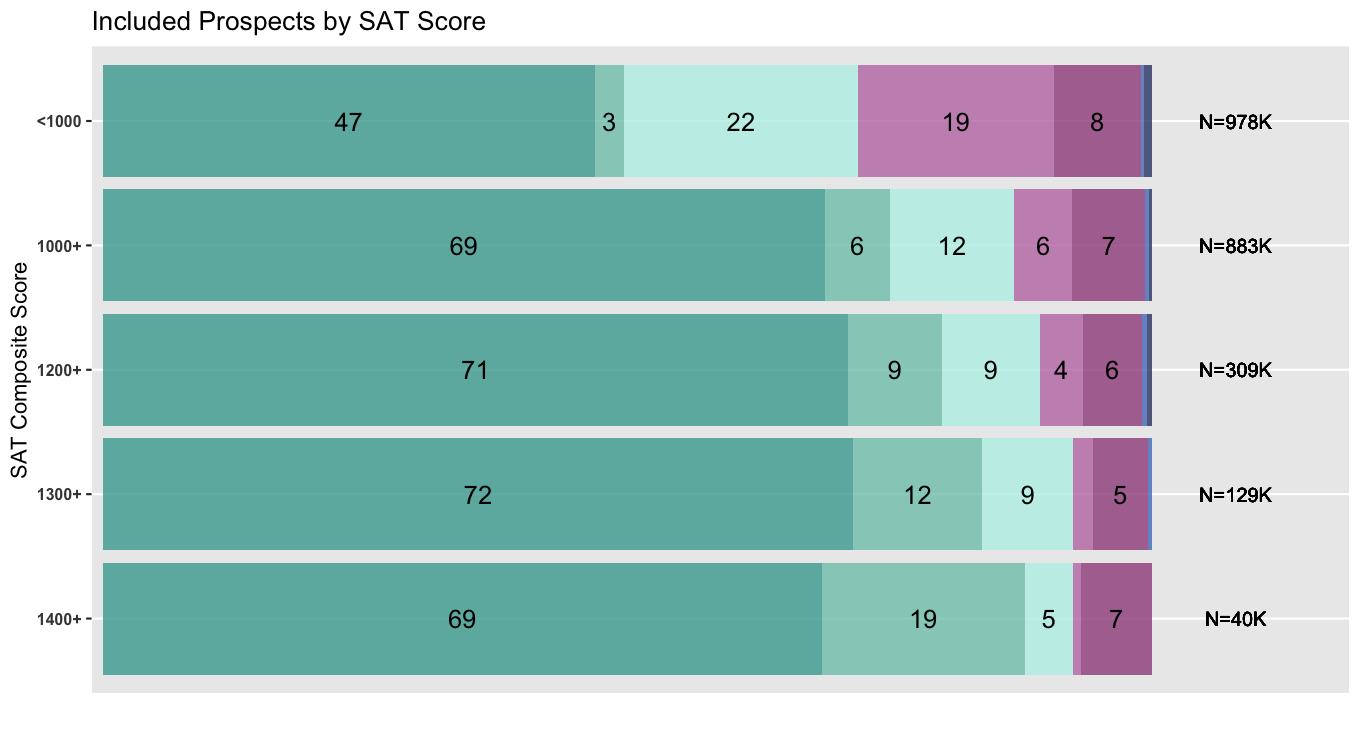
\includegraphics[width=0.35\linewidth]{./../../outputs/figures/p2_sat_incv2} 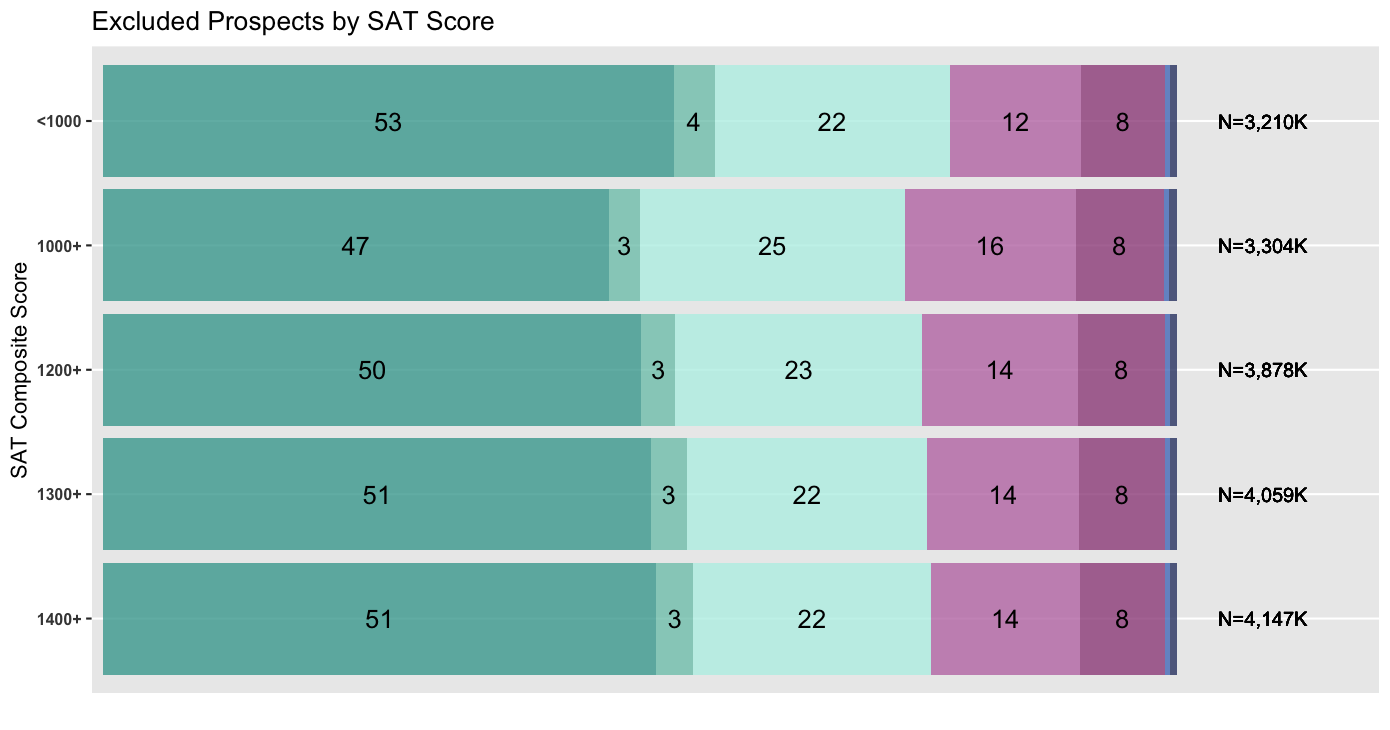
\includegraphics[width=0.35\linewidth]{./../../outputs/figures/p2_sat_excv2} 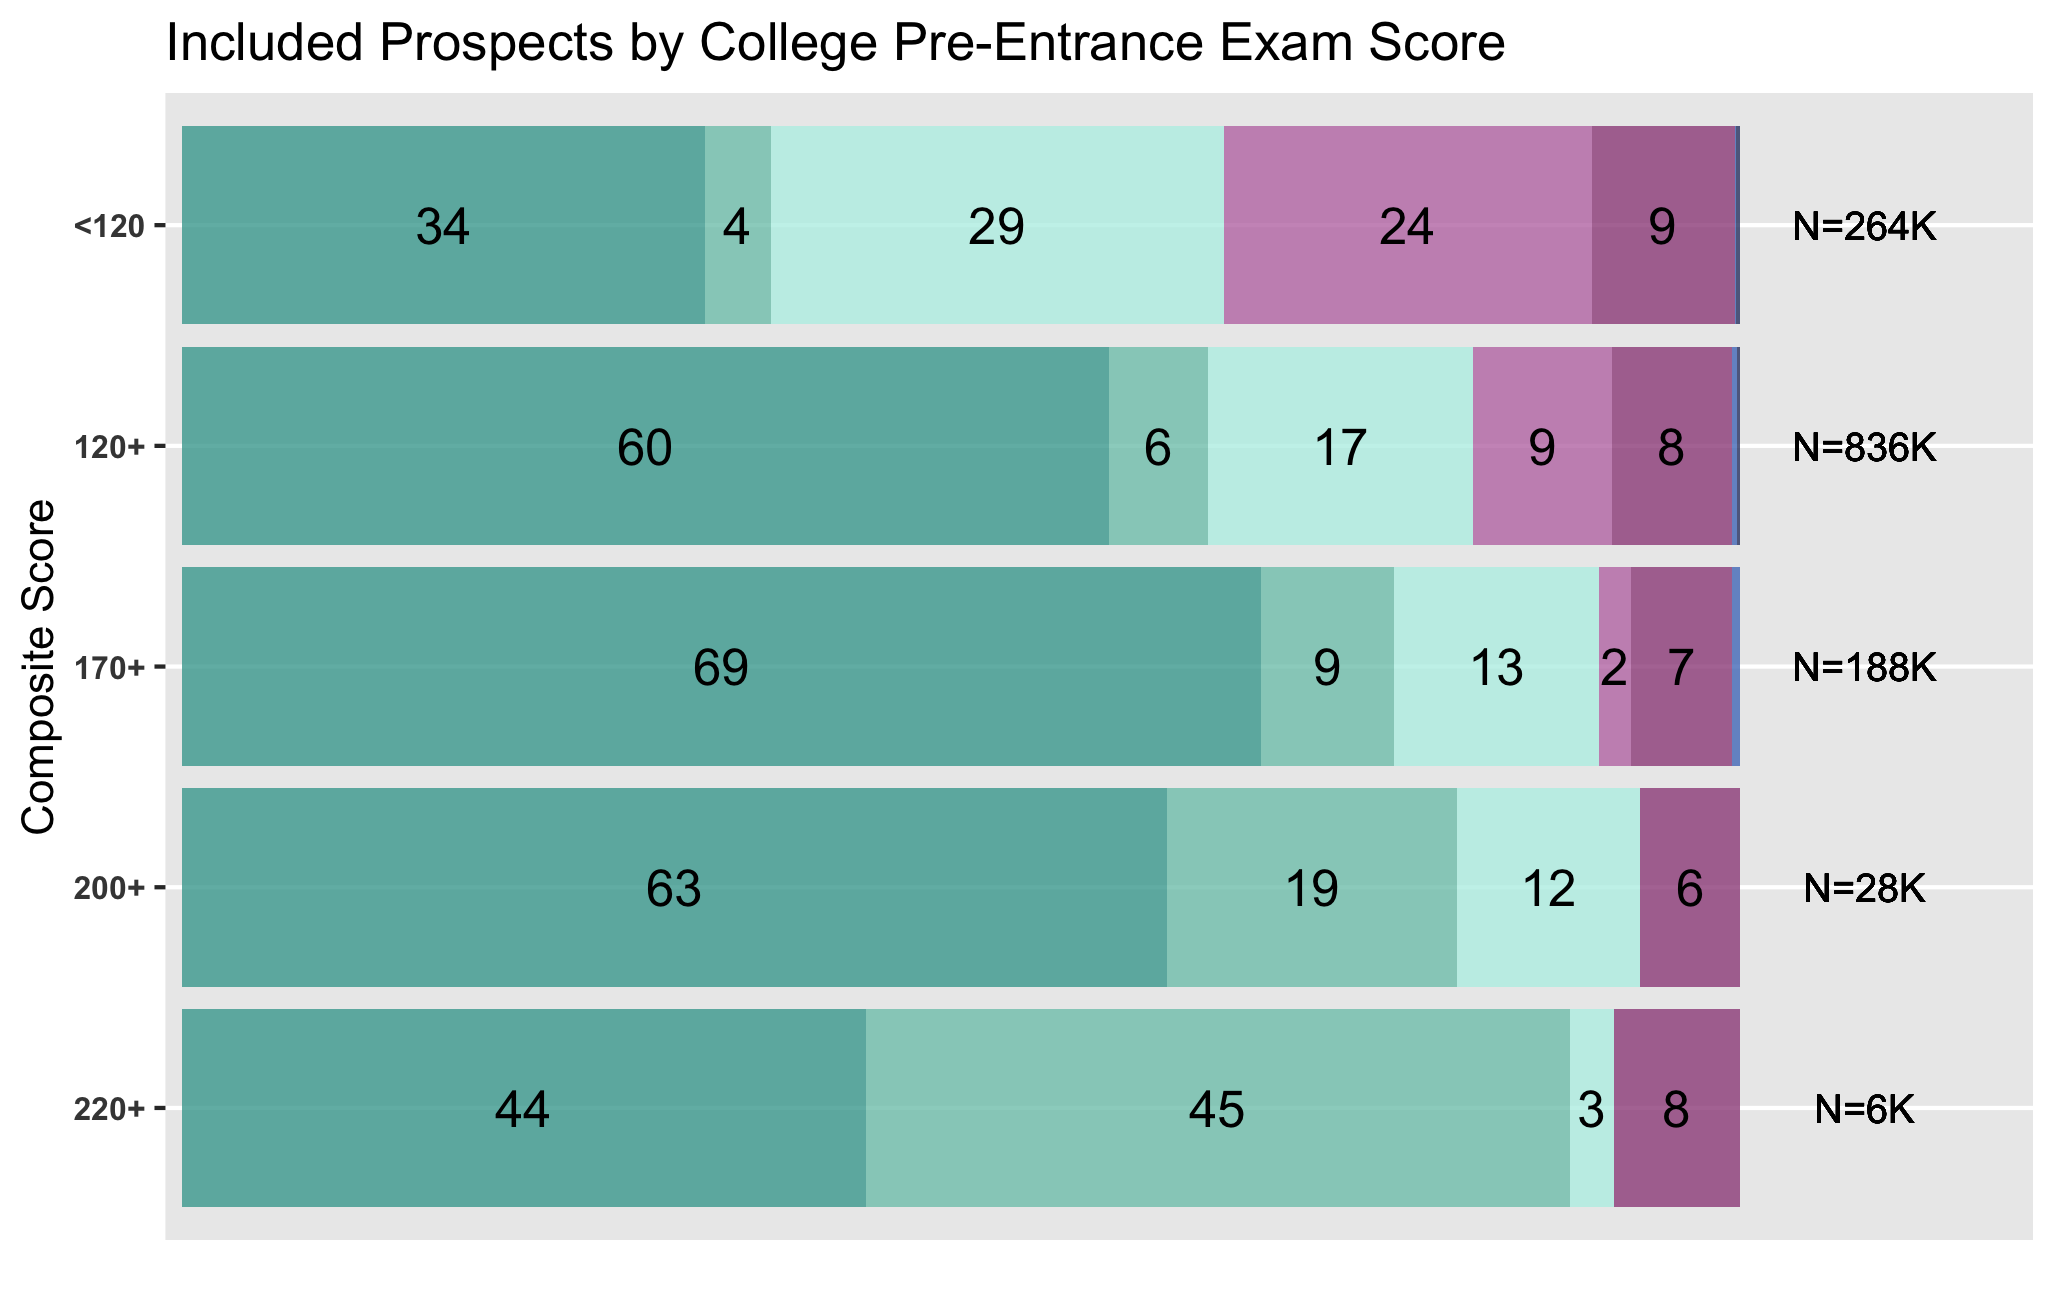
\includegraphics[width=0.35\linewidth]{./../../outputs/figures/p2_psat_incv2} 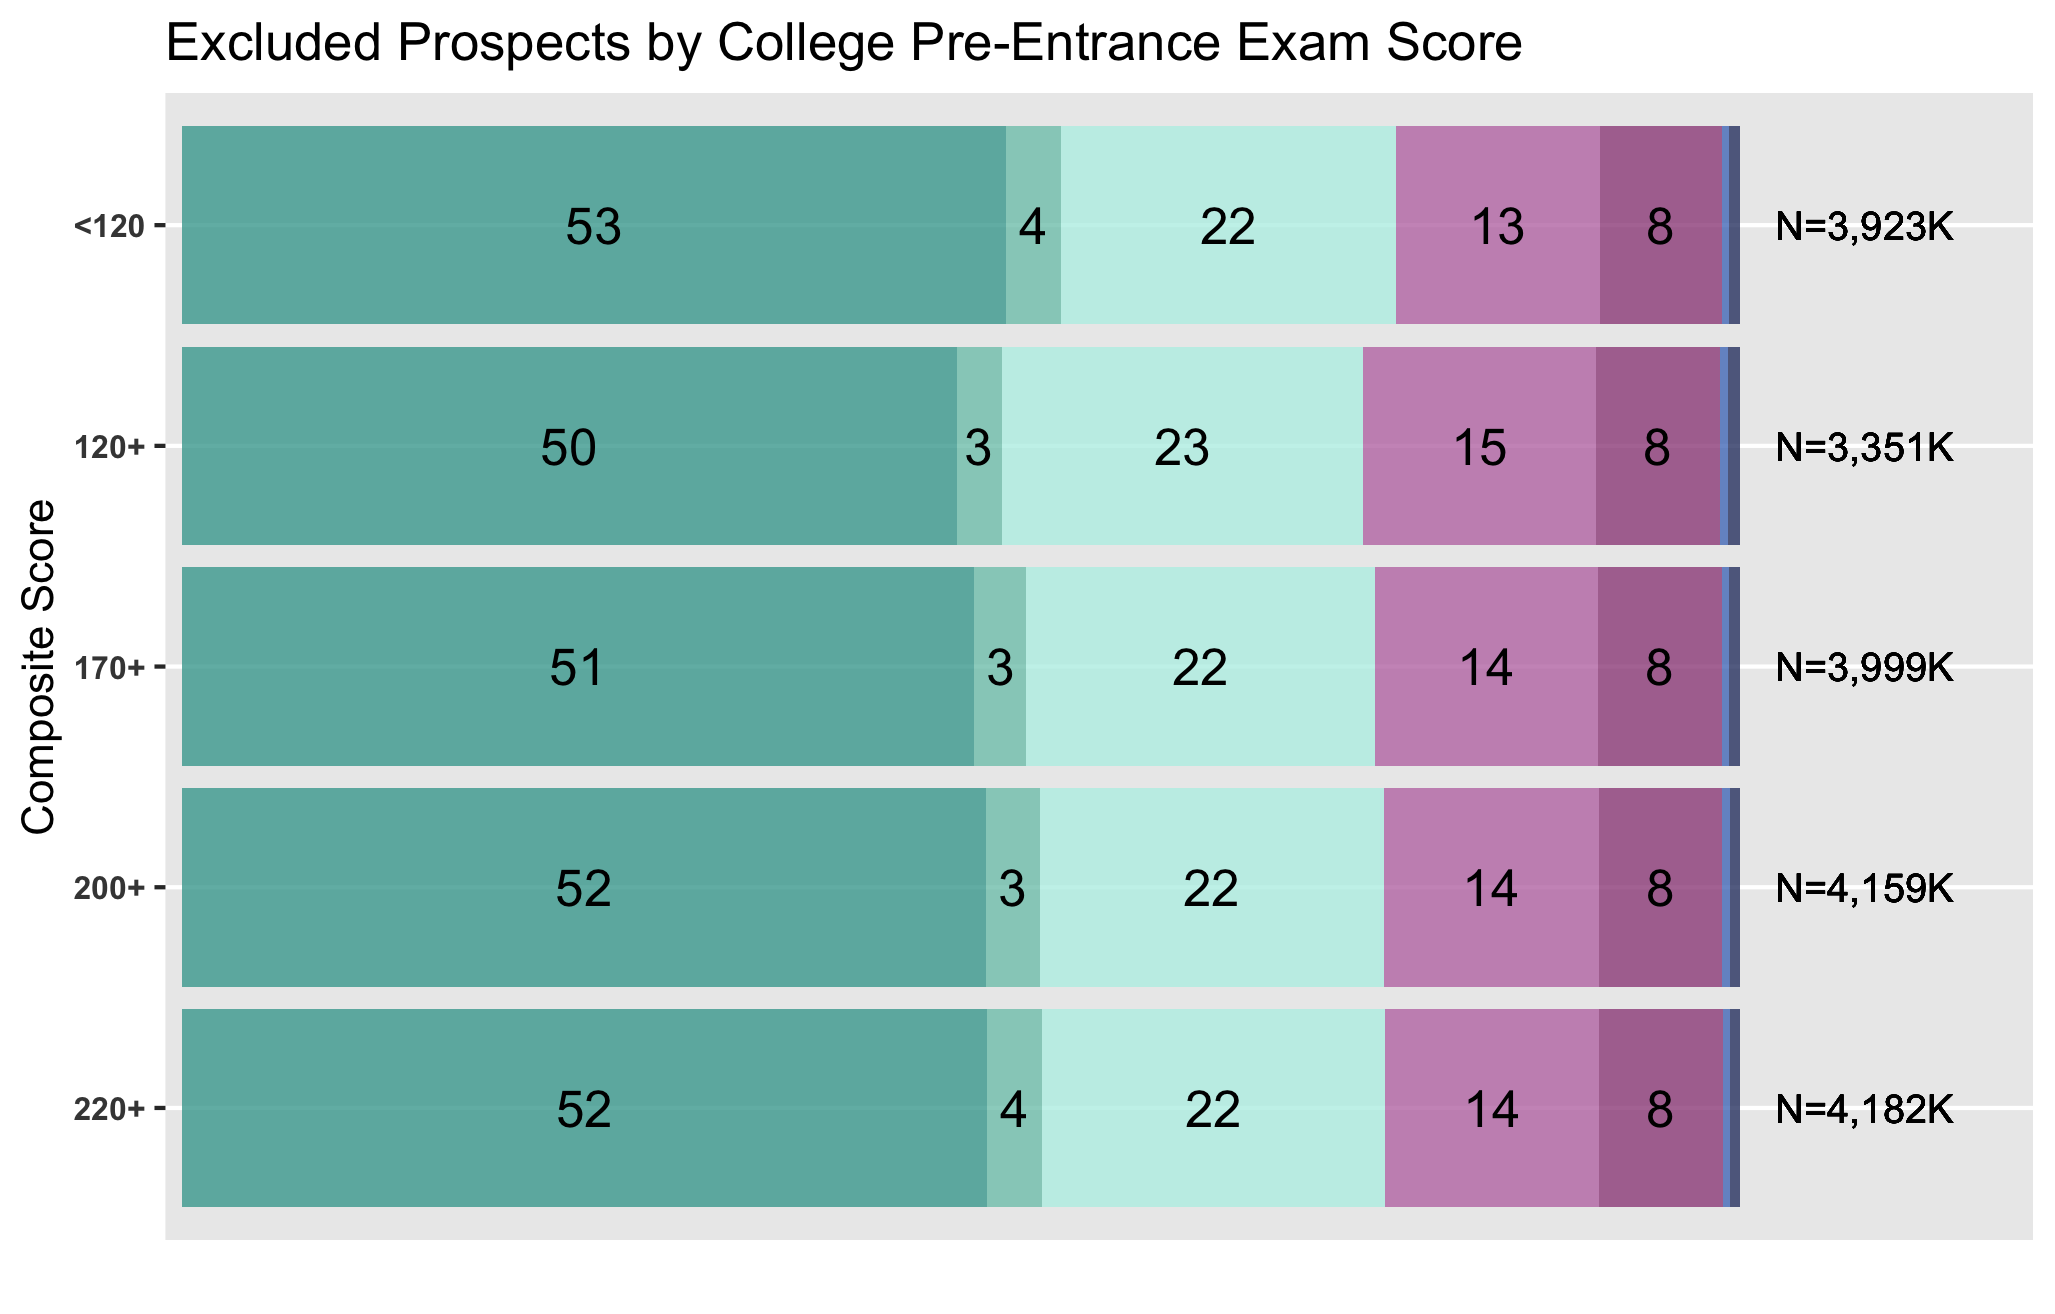
\includegraphics[width=0.35\linewidth]{./../../outputs/figures/p2_psat_excv2} 
\includegraphics[width=0.35\linewidth]{./../../outputs/figures/legend_horizontal} 

}

\caption{College Entrance and Pre-Entrance Exam Filters Across Thresholds}\label{fig:thresholds-tests}
\end{figure}

\begingroup
\fontsize{8}{8}\selectfont

SOURCE: U.S. Department of Education, National Center for Education Statistics, High School Longitudinal Study of 2009 (HSLS09).
\endgroup

\begin{figure}

{\centering 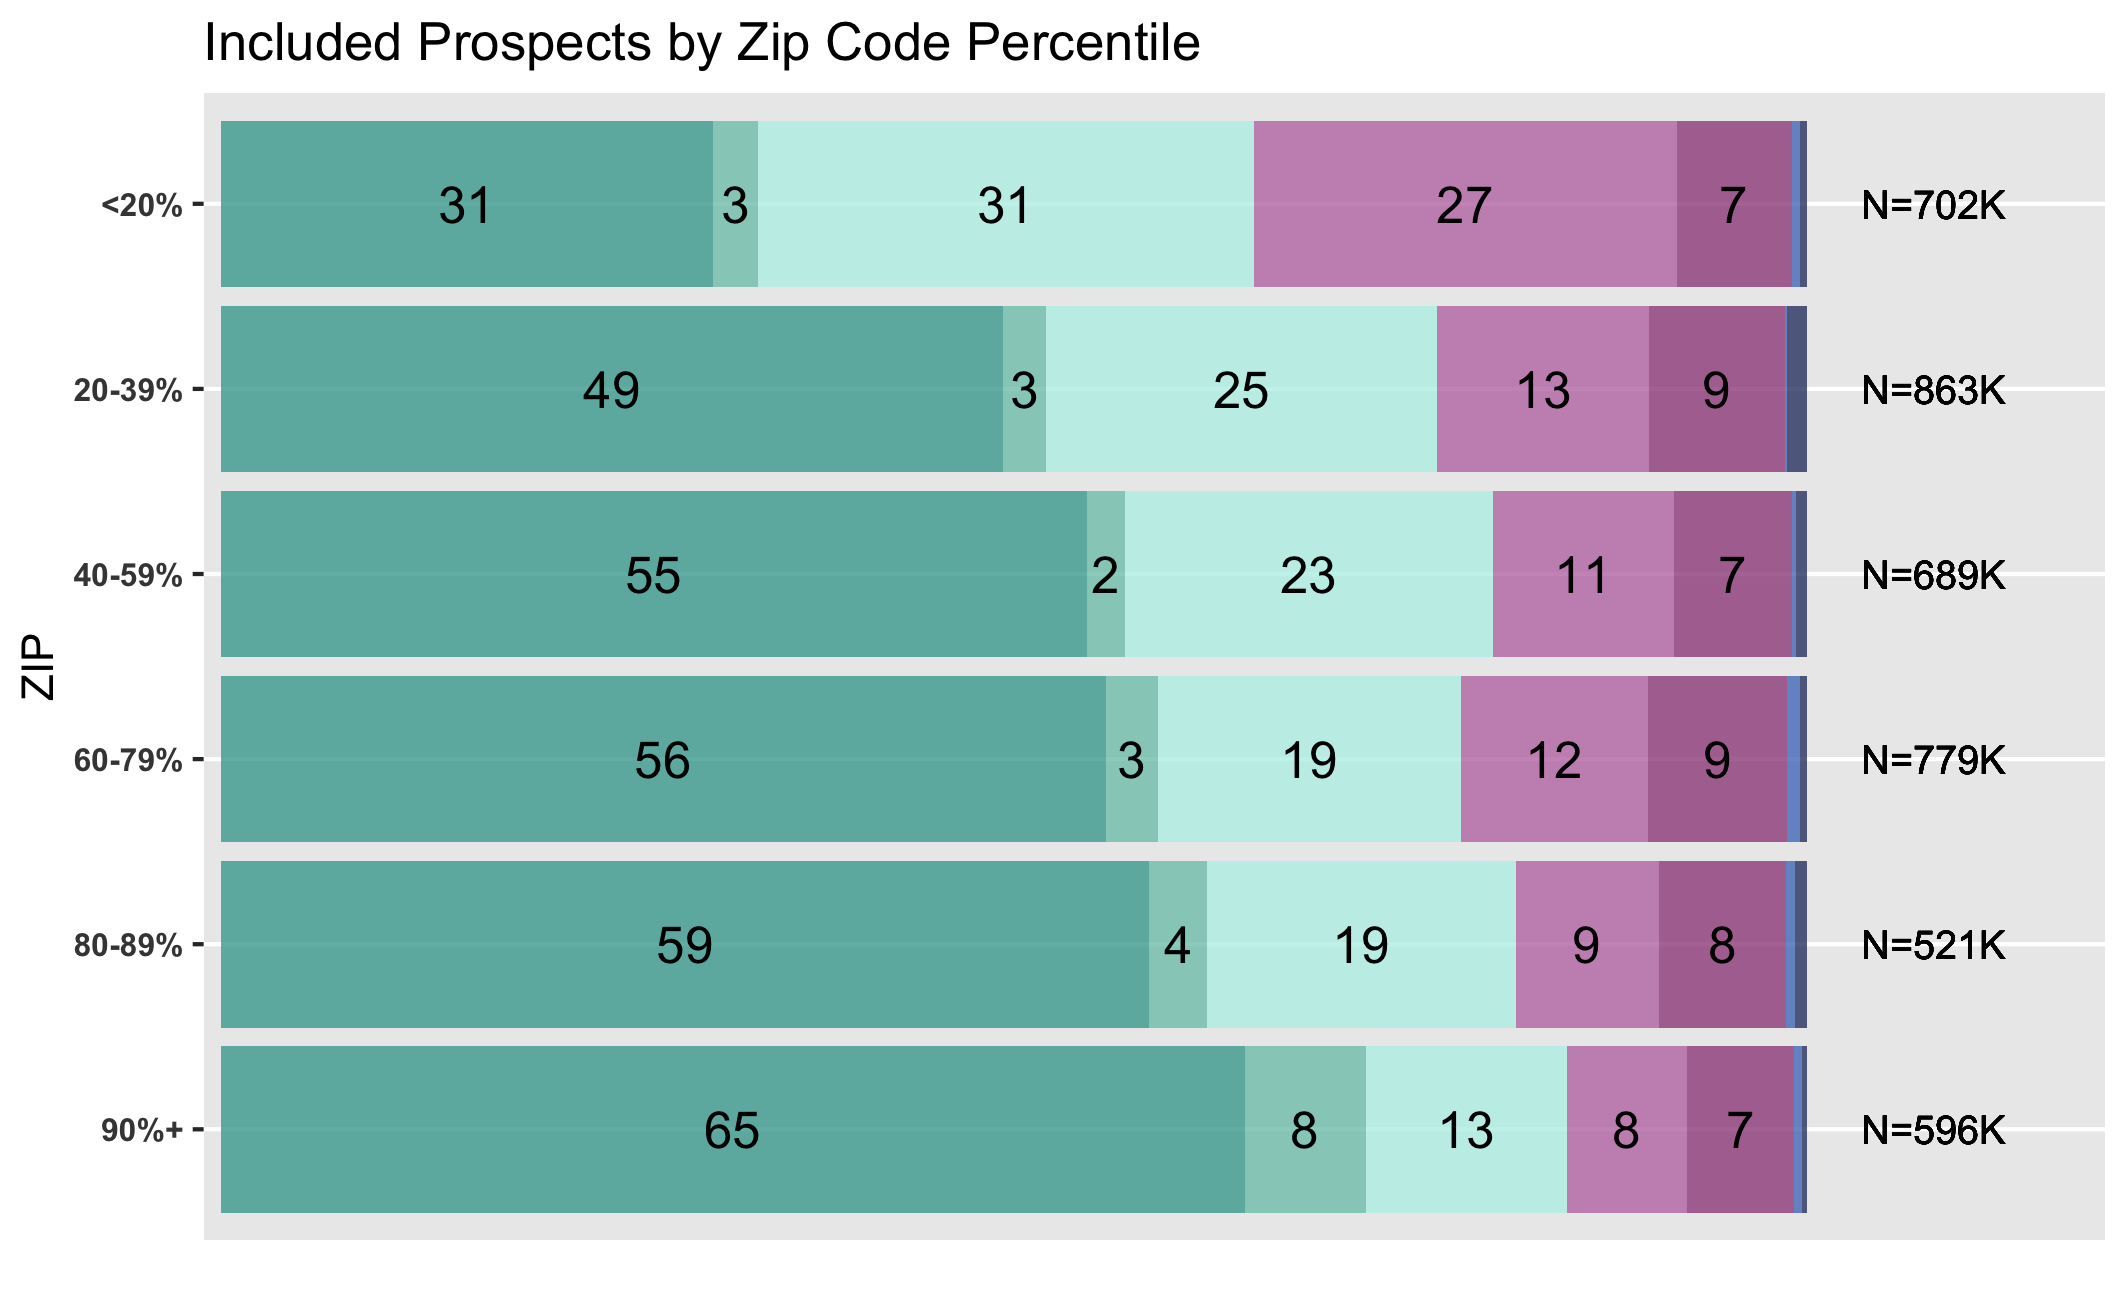
\includegraphics[width=0.4\linewidth]{./../../outputs/figures/p3_zip_incV2} 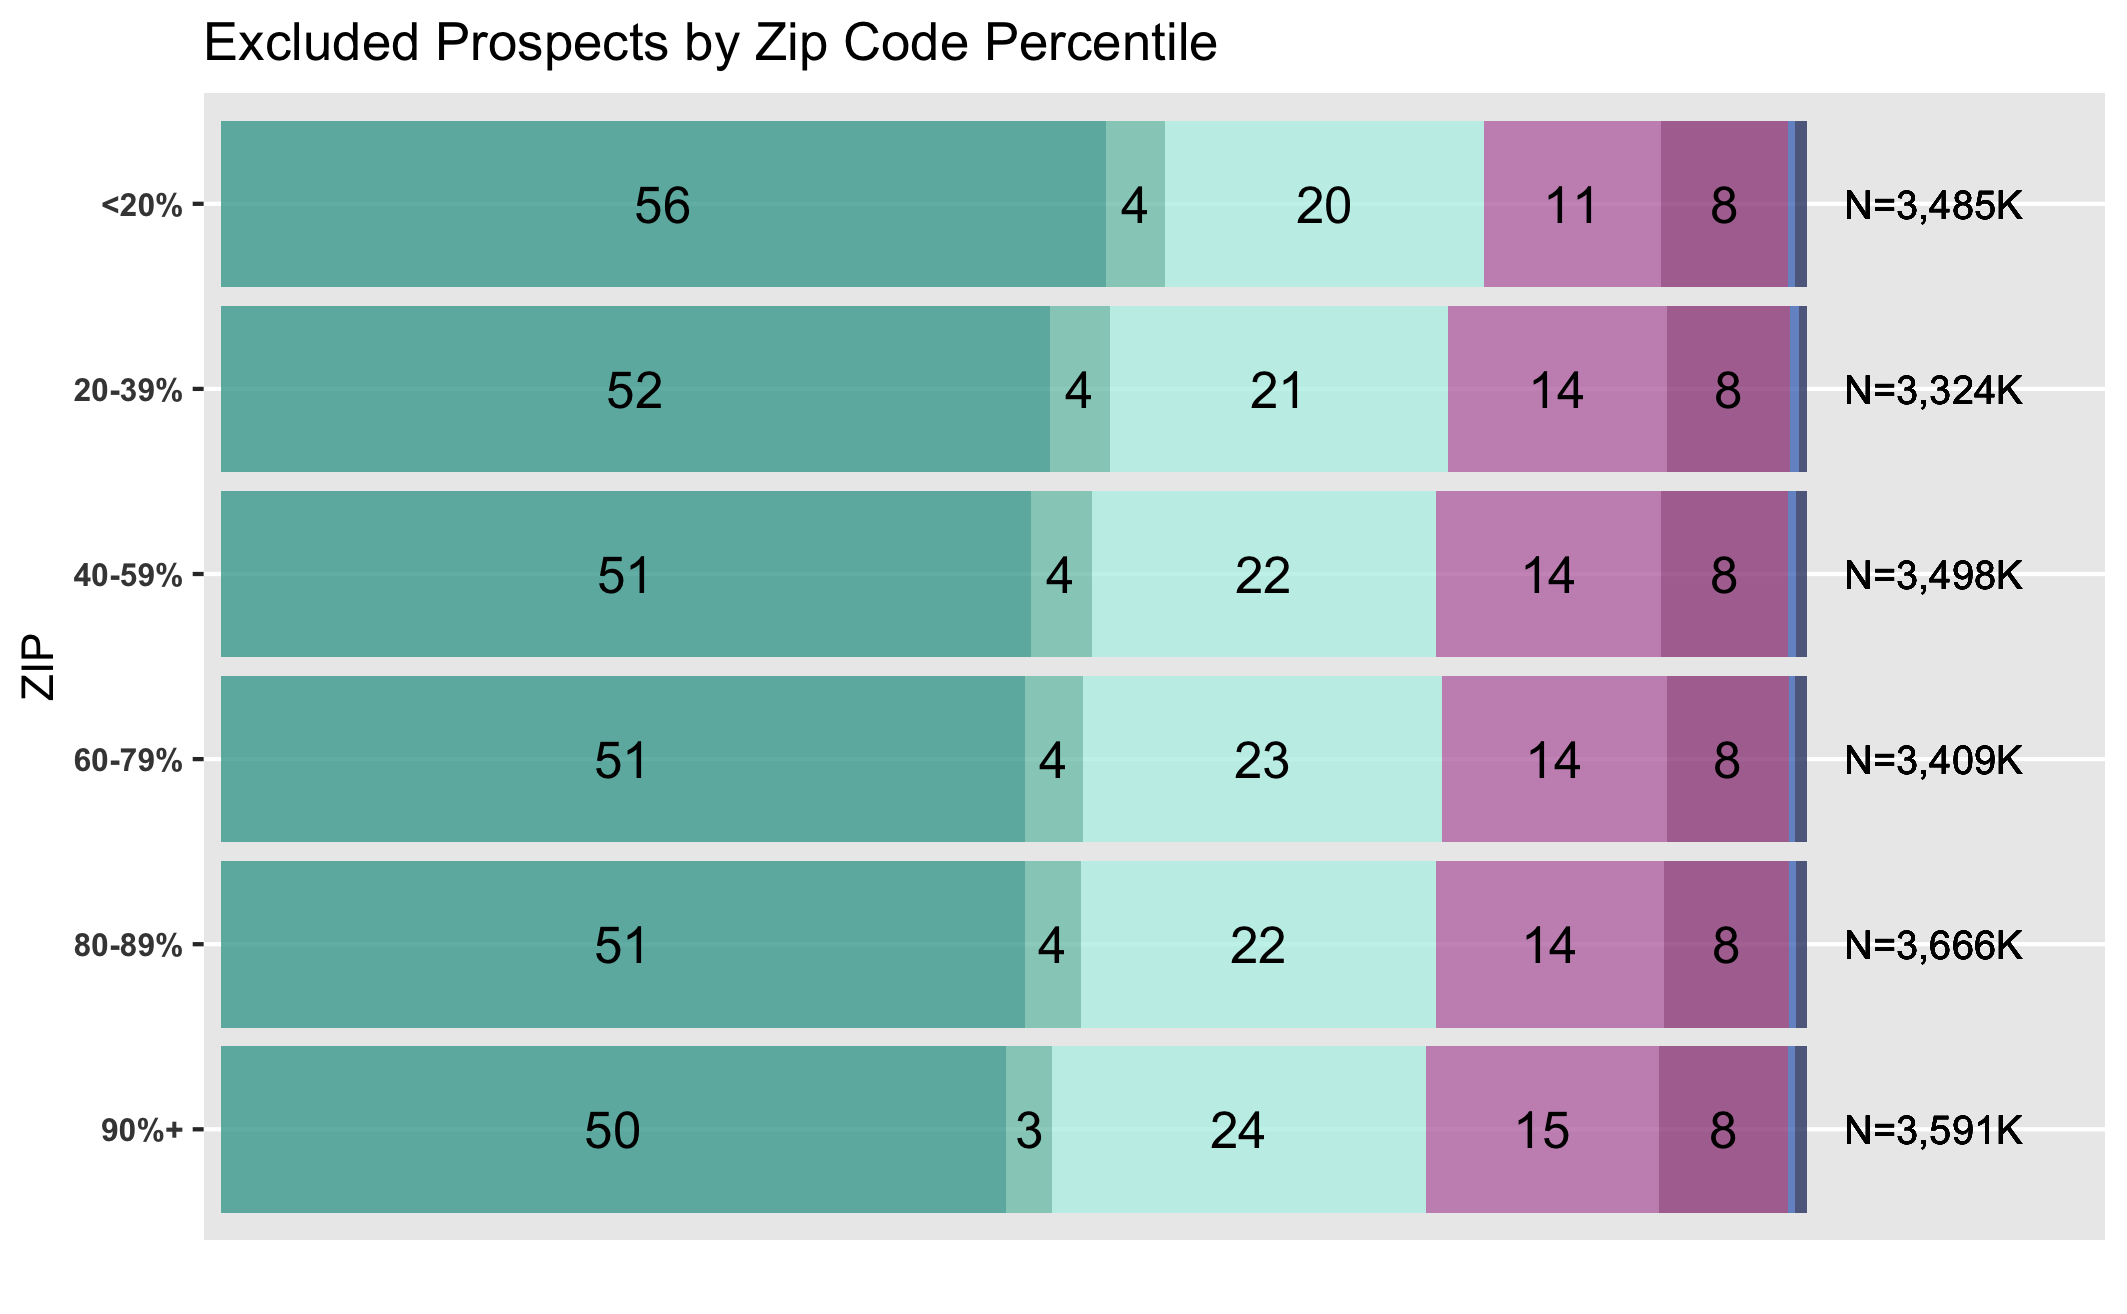
\includegraphics[width=0.4\linewidth]{./../../outputs/figures/p3_zip_excV2} 
\includegraphics[width=0.4\linewidth]{./../../outputs/figures/legend_horizontal} 

}

\caption{Zip Code Filter Across Affluence Percentiles}\label{fig:zipcode-affluence}
\end{figure}

\begingroup
\fontsize{8}{8}\selectfont

SOURCE: U.S. Department of Education, National Center for Education Statistics, High School Longitudinal Study of 2009 (HSLS09).
\endgroup

\textbackslash end\{landscape\}
\pagebreak
\restoregeometry

\begin{figure}
\centering
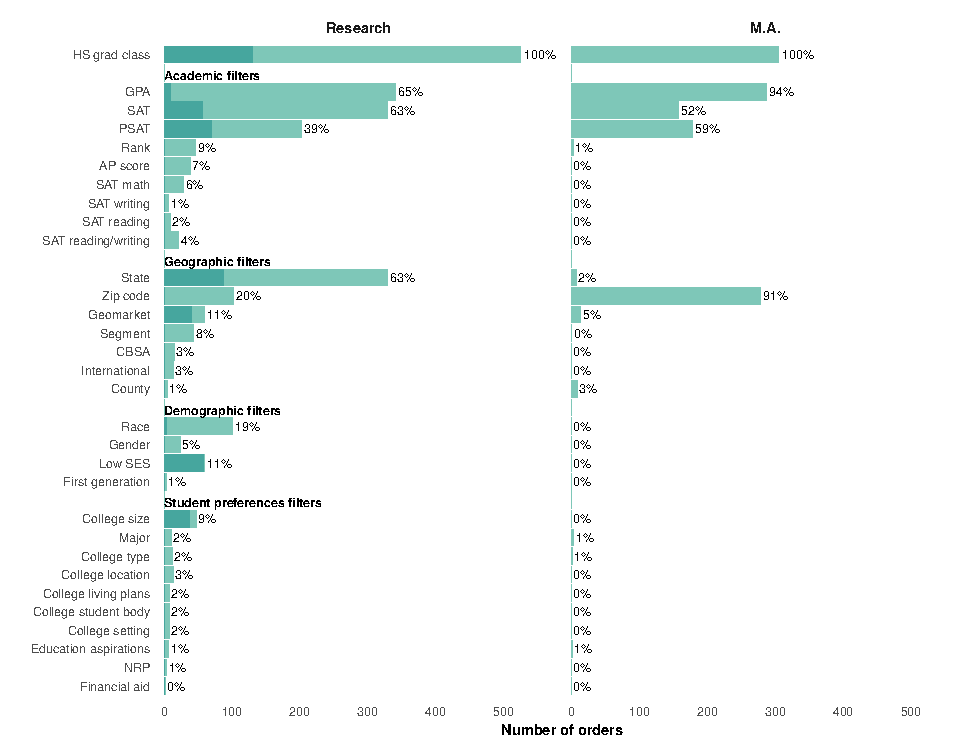
\includegraphics{eepa_student_list_manuscript_c_a_files/figure-latex/order-filters-empirical-report-1.pdf}
\caption{\label{fig:order-filters-empirical-report}Filters used in College Board Orders Purchased by 14 Public Universities}
\end{figure}

\begingroup
\fontsize{8}{8}\selectfont

NOTE: One research university placed a large amount of orders, which influenced the overall filters used for all research universities. The contribution of this particular university is shown in the darker color in the figure.
\endgroup

\begin{figure}
\centering
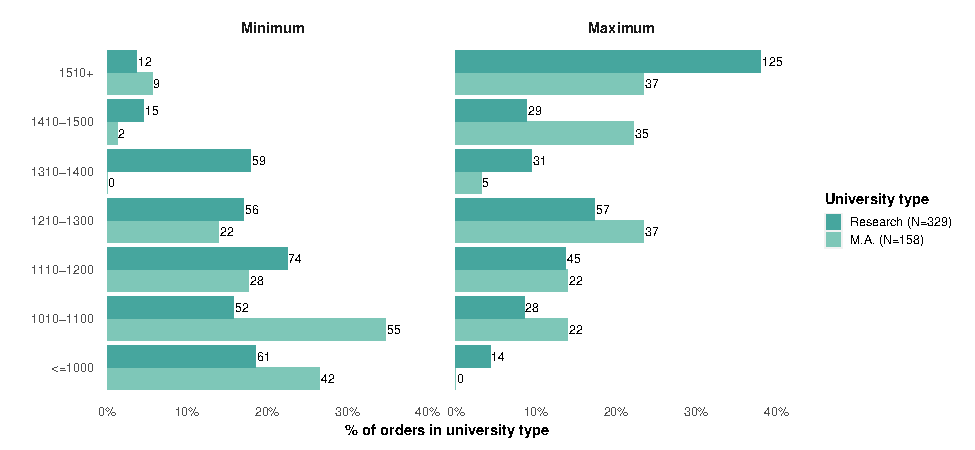
\includegraphics{eepa_student_list_manuscript_c_a_files/figure-latex/orders-sat-1.pdf}
\caption{\label{fig:orders-sat}SAT Filter Used by Research vs.~Master's Public Universities}
\end{figure}

\pagebreak

\begin{landscape}



\begin{figure}

{\centering 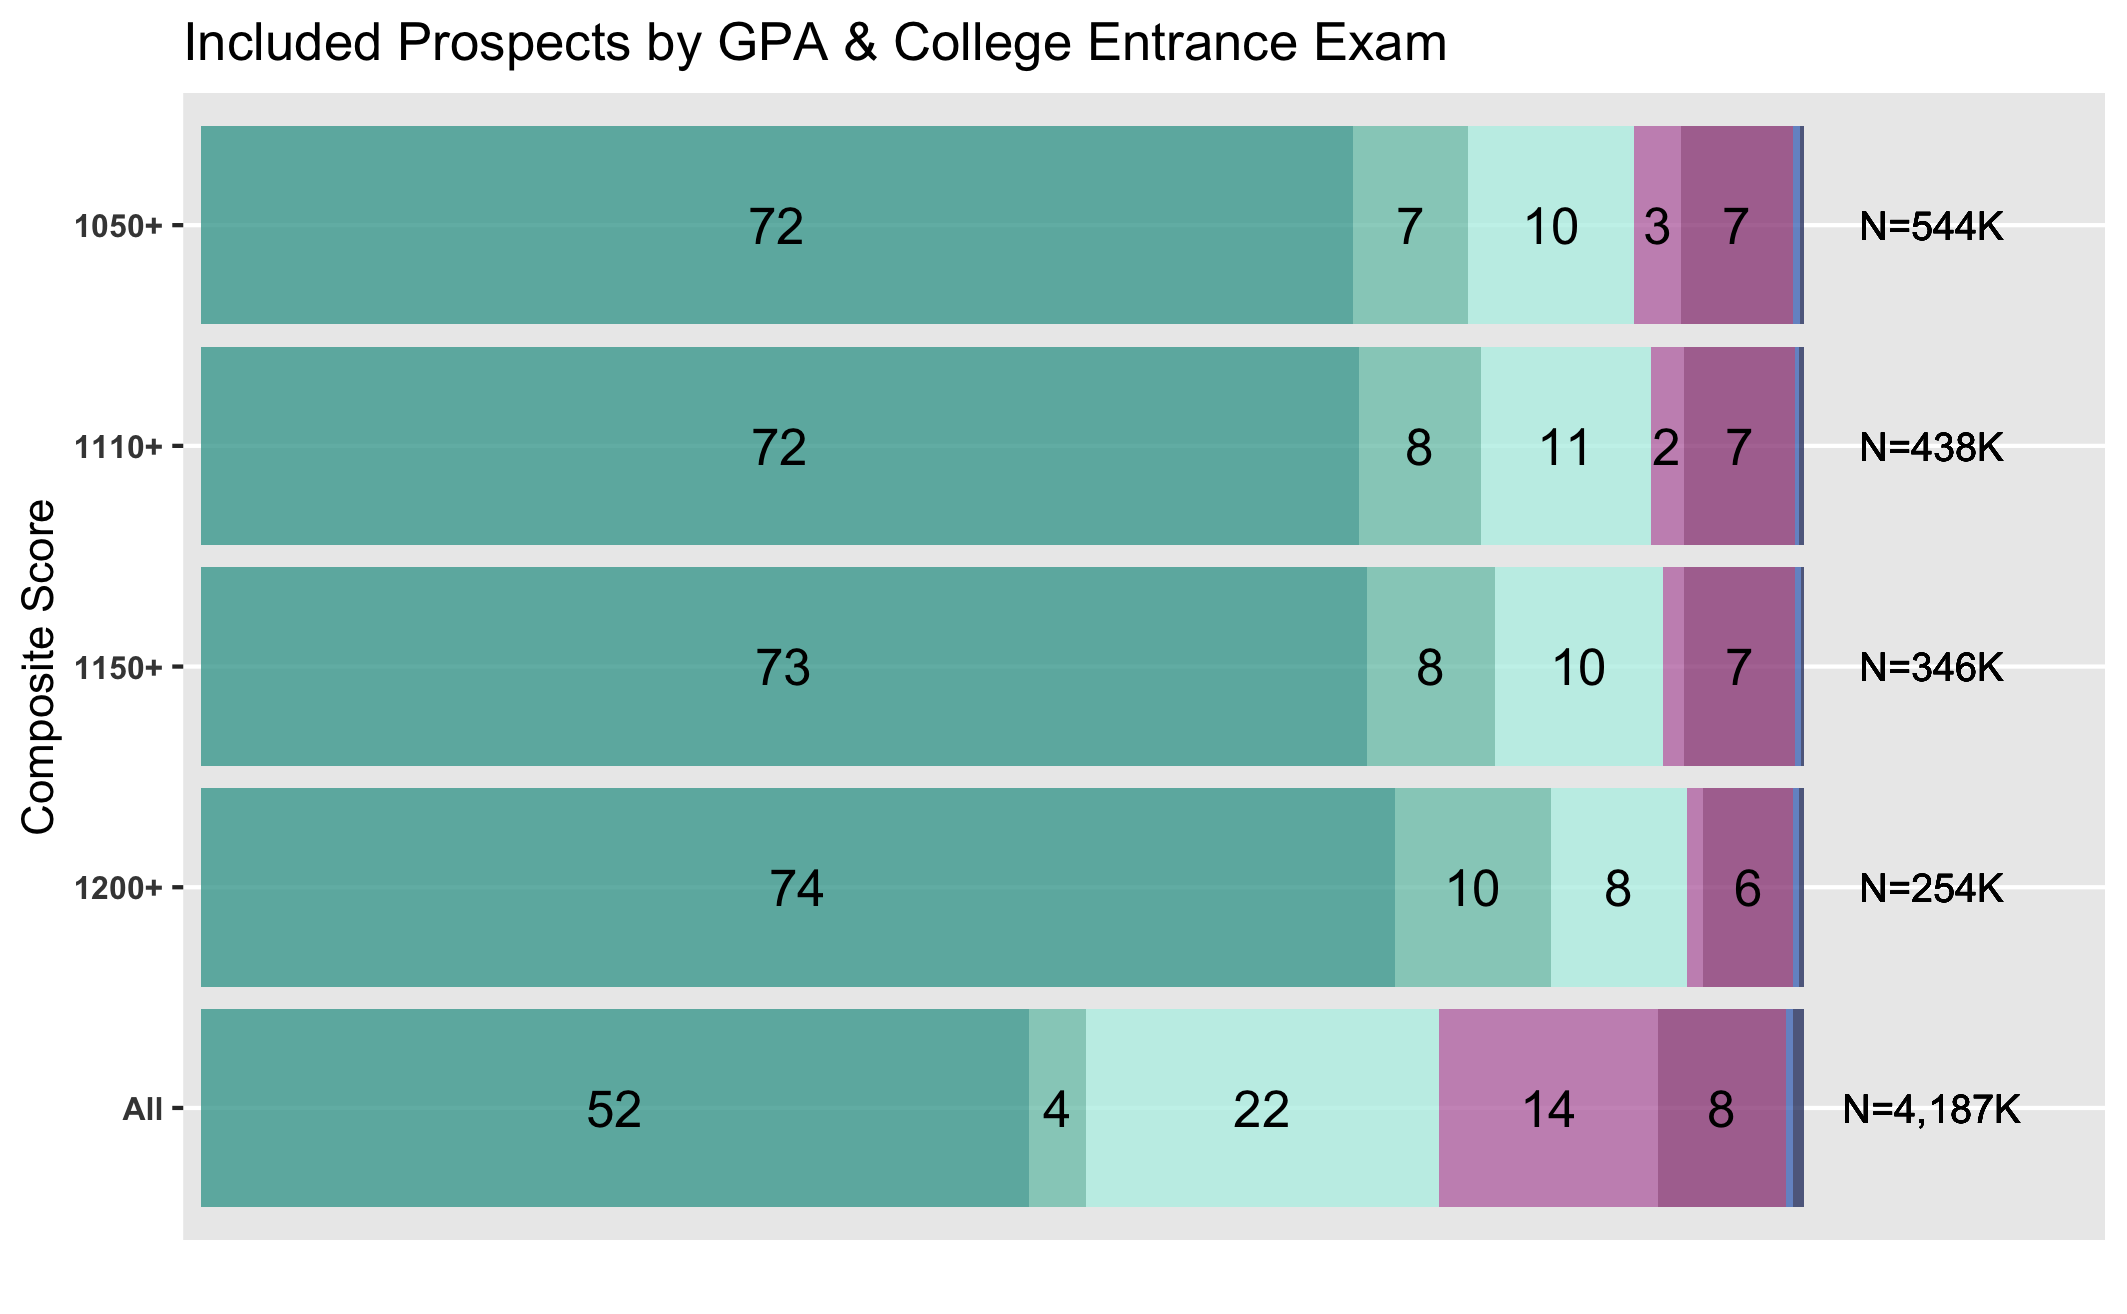
\includegraphics[width=3in]{./../../outputs/figures/combo1_inc_satv2} 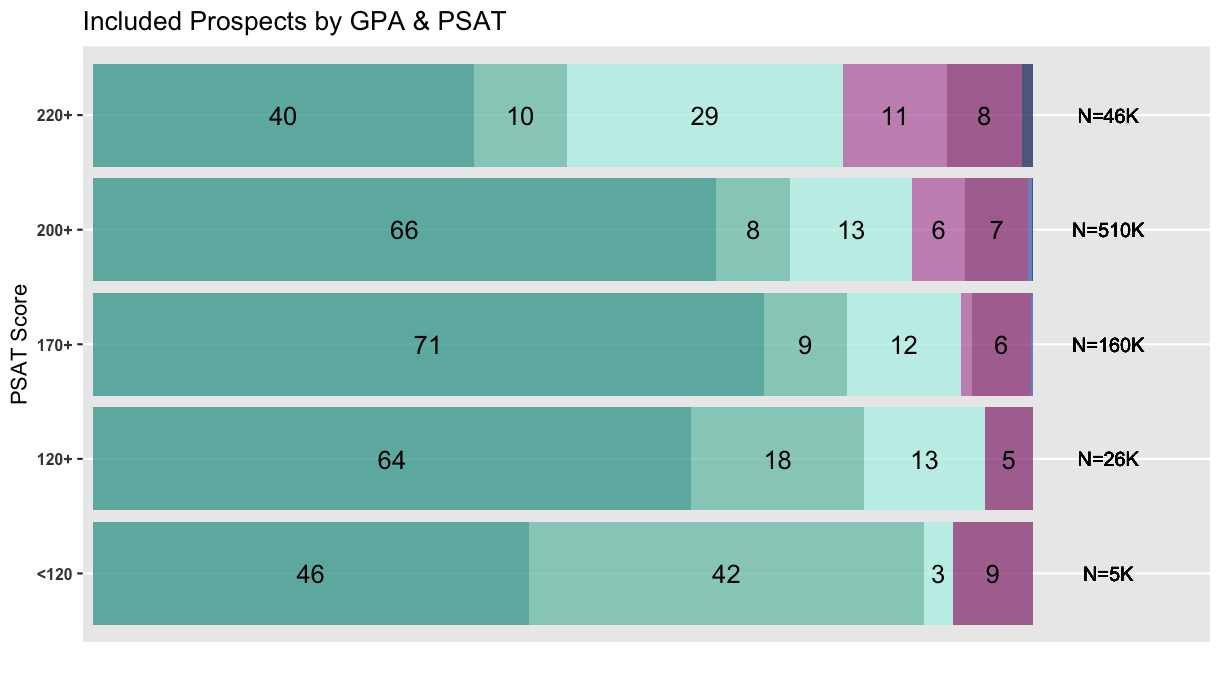
\includegraphics[width=3in]{./../../outputs/figures/combo1_inc_psatv2} 

}

\caption{Academic Combinations: GPA (3.0+) and College Entrance or Pre-Entrance Exams (across score thresholds)}\label{fig:gpa-sat-psat}
\end{figure}


\begin{center}
\includegraphics[width=0.32\linewidth]{./../../outputs/figures/legend_horizontal} \end{center}

\begingroup
\fontsize{8}{8}\selectfont
SOURCE: U.S. Department of Education, National Center for Education Statistics, High School Longitudinal Study of 2009 (HSLS09).
\endgroup

\pagebreak


\begin{figure}

{\centering 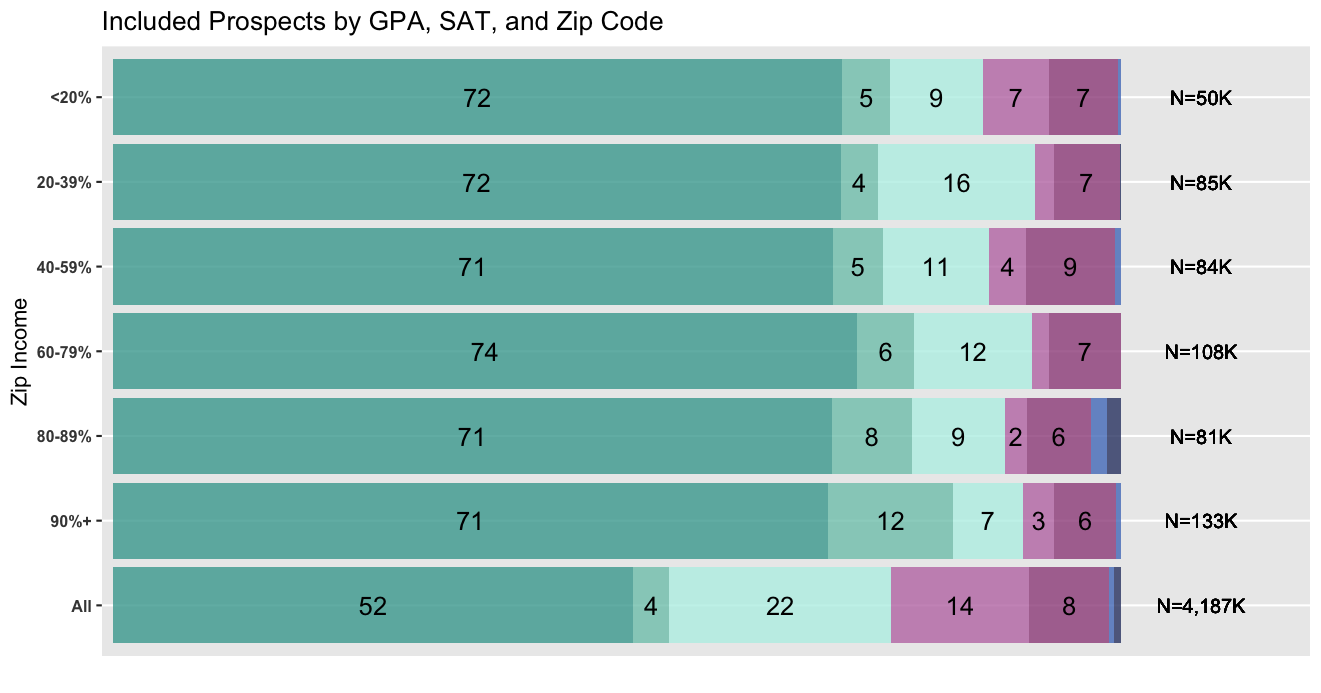
\includegraphics[width=0.35\linewidth]{./../../outputs/figures/combo2_inc_satV2} 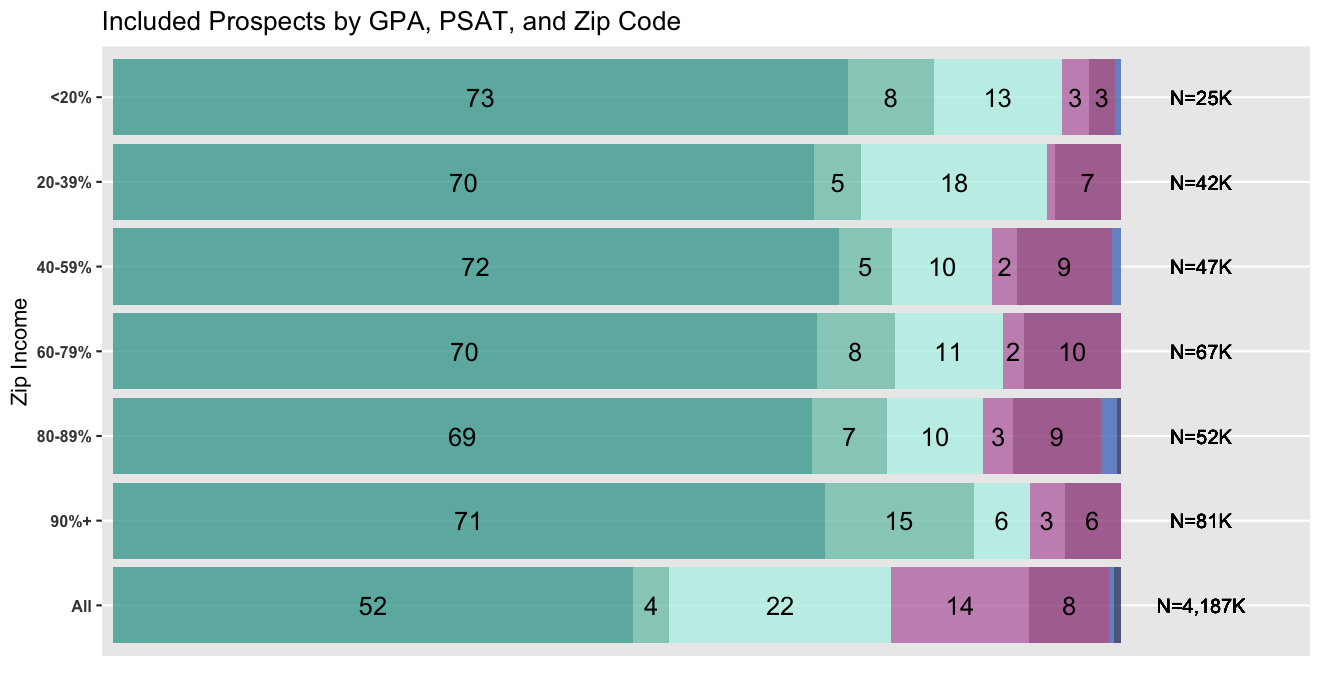
\includegraphics[width=0.35\linewidth]{./../../outputs/figures/combo2_inc_psatV2} 

}

\caption{Academic and Geographic Combination: GPA (3.0+), College Pre-Entrance (150+) or Entrance (1050+) Exams, and Zip (across income thresholds)}\label{fig:gpa-sat-psat-zip}
\end{figure}


\begin{center}
\includegraphics[width=0.32\linewidth]{./../../outputs/figures/legend_horizontal} \end{center}

\begingroup
\fontsize{8}{8}\selectfont
SOURCE: U.S. Department of Education, National Center for Education Statistics, High School Longitudinal Study of 2009 (HSLS09).
\endgroup

\end{landscape}

\restoregeometry

\clearpage

\begin{figure}
\centering
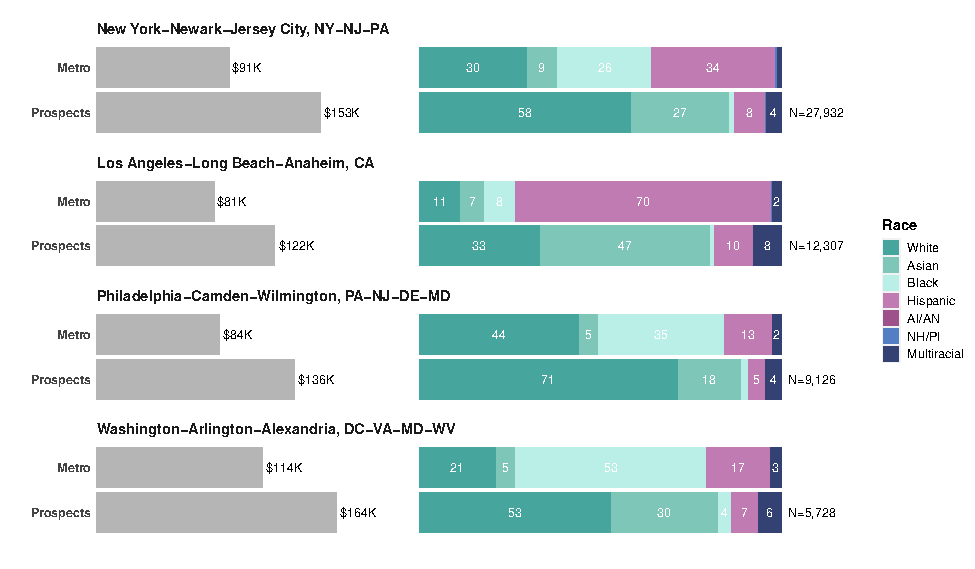
\includegraphics{eepa_student_list_manuscript_c_a_files/figure-latex/uiuc-deep-dive-1.pdf}
\caption{\label{fig:uiuc-deep-dive}Segment Filter Prospects by Metropolitan Area}
\end{figure}

\begingroup
\fontsize{10}{10}\selectfont

\emph{Note: Filters used across these orders include HS Class, GPA (B-A+), State (in-state vs.~out-of-state), AP STEM (3 min for in-state; 4 min for out-of-state) or SAT (1200 minimum for in-state; 1300 minimum for out-of-state) with STEM major interest. Metro population source is the National Center for Education Statistic's Common Core of Data and includes all students attending a public high school in the metropolitan area. }
\endgroup

\pagebreak

\begin{landscape}

\begin{figure}

{\centering 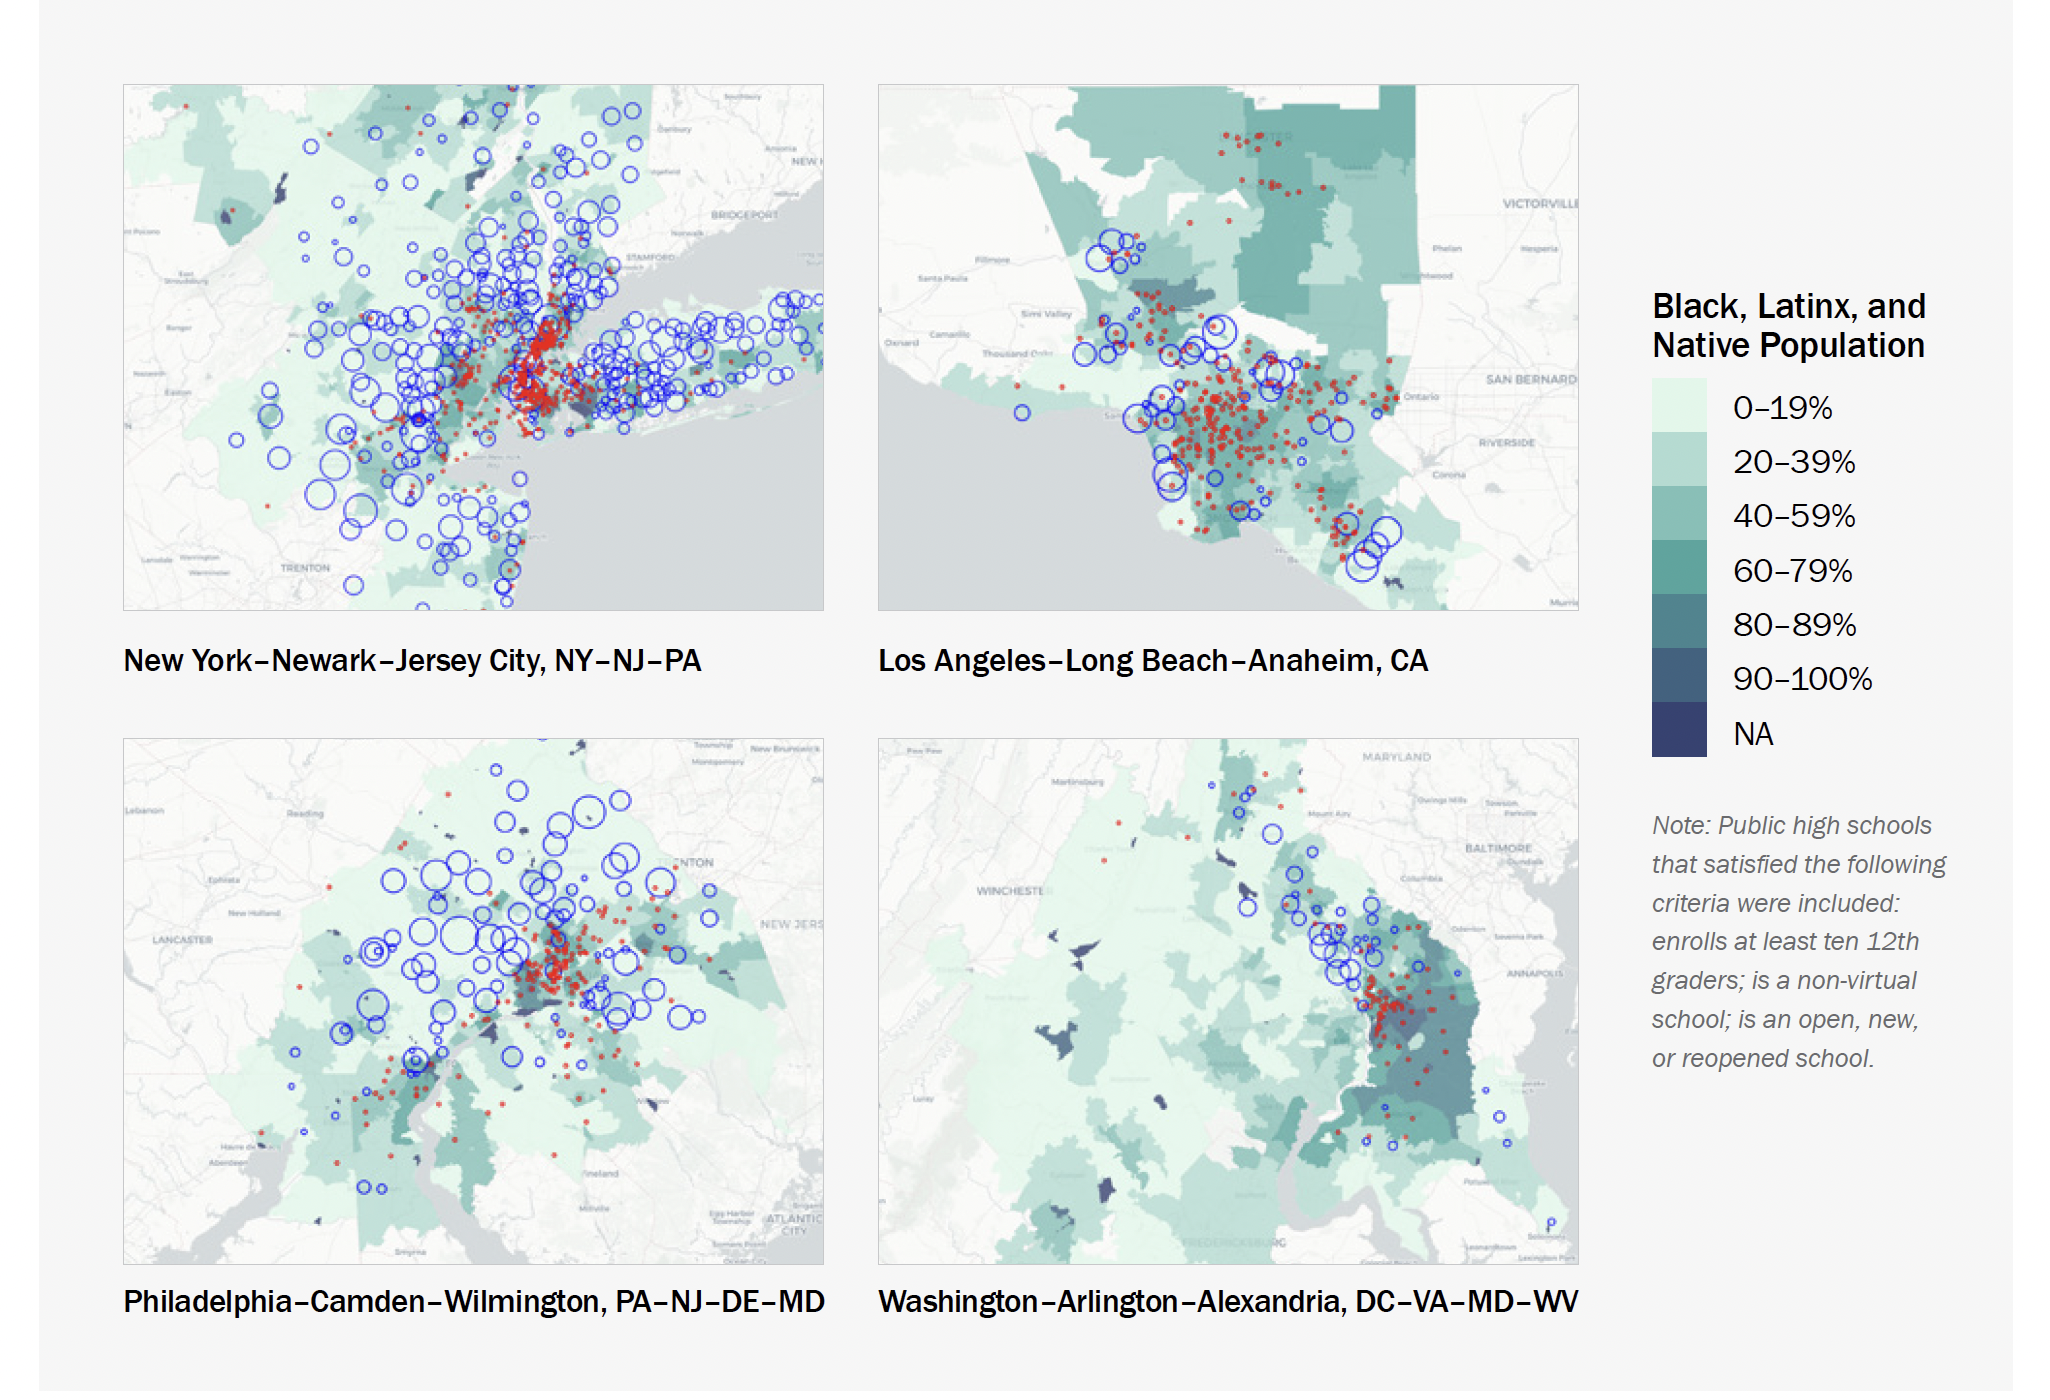
\includegraphics[width=1\linewidth]{./../../outputs/images/uiuc-map} 

}

\caption{Maps of Segment Filter Prospects by Metropolitan Area}\label{fig:uiuc-map}
\end{figure}

\end{landscape}

\pagebreak

\clearpage

\begin{figure}
\centering
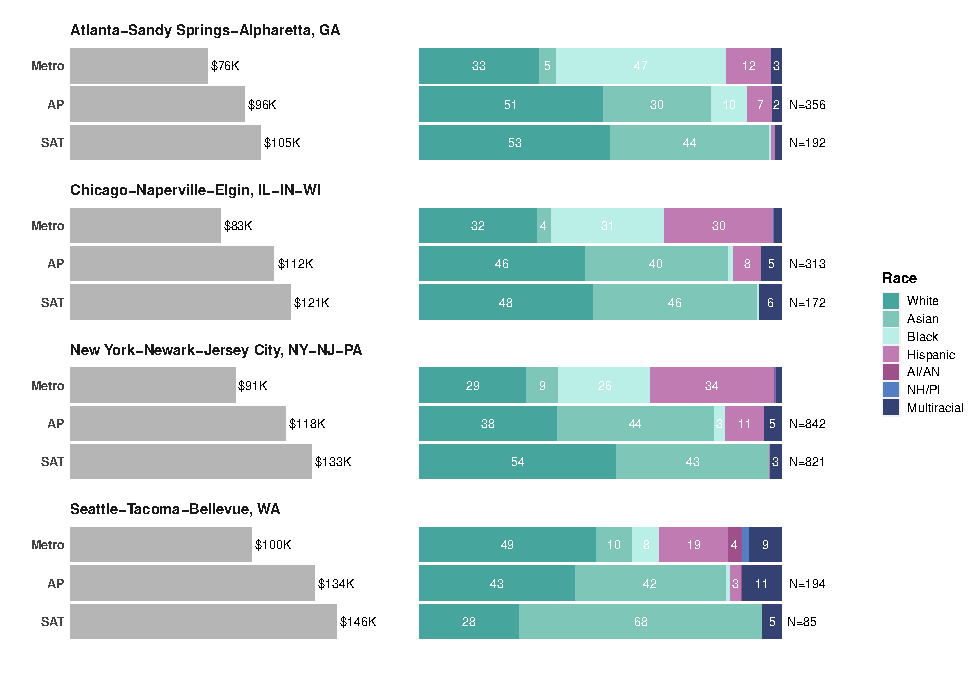
\includegraphics{eepa_student_list_manuscript_c_a_files/figure-latex/ucsd-deep-dive-1.pdf}
\caption{\label{fig:ucsd-deep-dive}Women in STEM Prospects by Metropolitan Area}
\end{figure}

\begingroup
\fontsize{10}{10}\selectfont

\emph{Note: Filters used across these orders include HS Class, Segment, GPA (B-A+), PSAT/SAT (1220-1450); State/CBSAs. Metro population source is the National Center for Education Statistic's Common Core of Data and includes all students attending a public high school in the metropolitan area. }
\endgroup

\newpage

\hypertarget{supplemental-online-appendix}{%
\section{Supplemental Online Appendix}\label{supplemental-online-appendix}}

\pagenumbering{gobble}
\pagenumbering{arabic}
\renewcommand*{\thepage}{A\arabic{page}}
\pagestyle{fancy}
\setlength{\headheight}{15pt}

\beginsupplement

\begin{figure}

{\centering 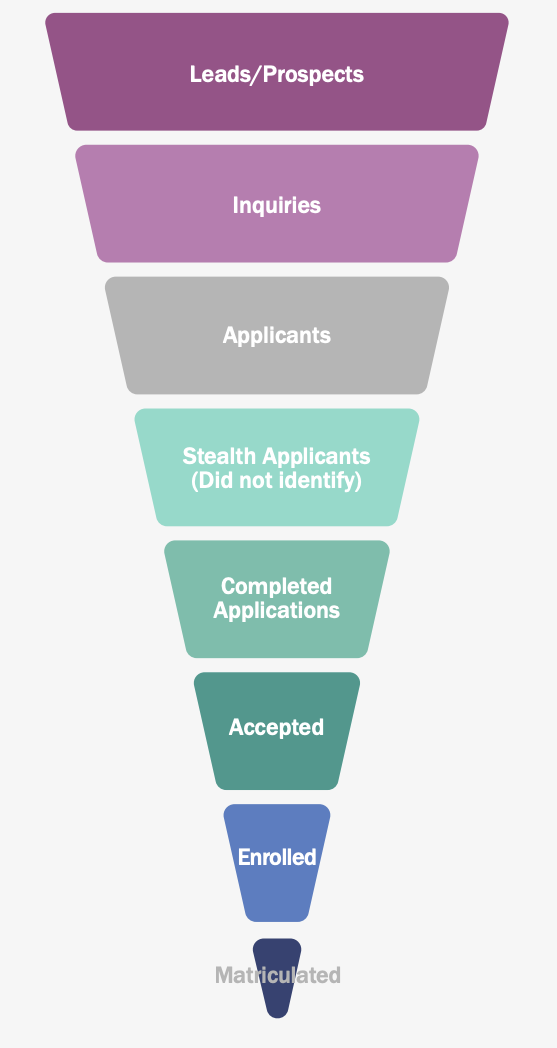
\includegraphics[width=0.45\linewidth]{./../../outputs/images/enroll_funnelv2} 

}

\caption{The Enrollment Funnel}\label{fig:em-funnel}
\end{figure}

\begin{landscape}


\begin{figure}

{\centering 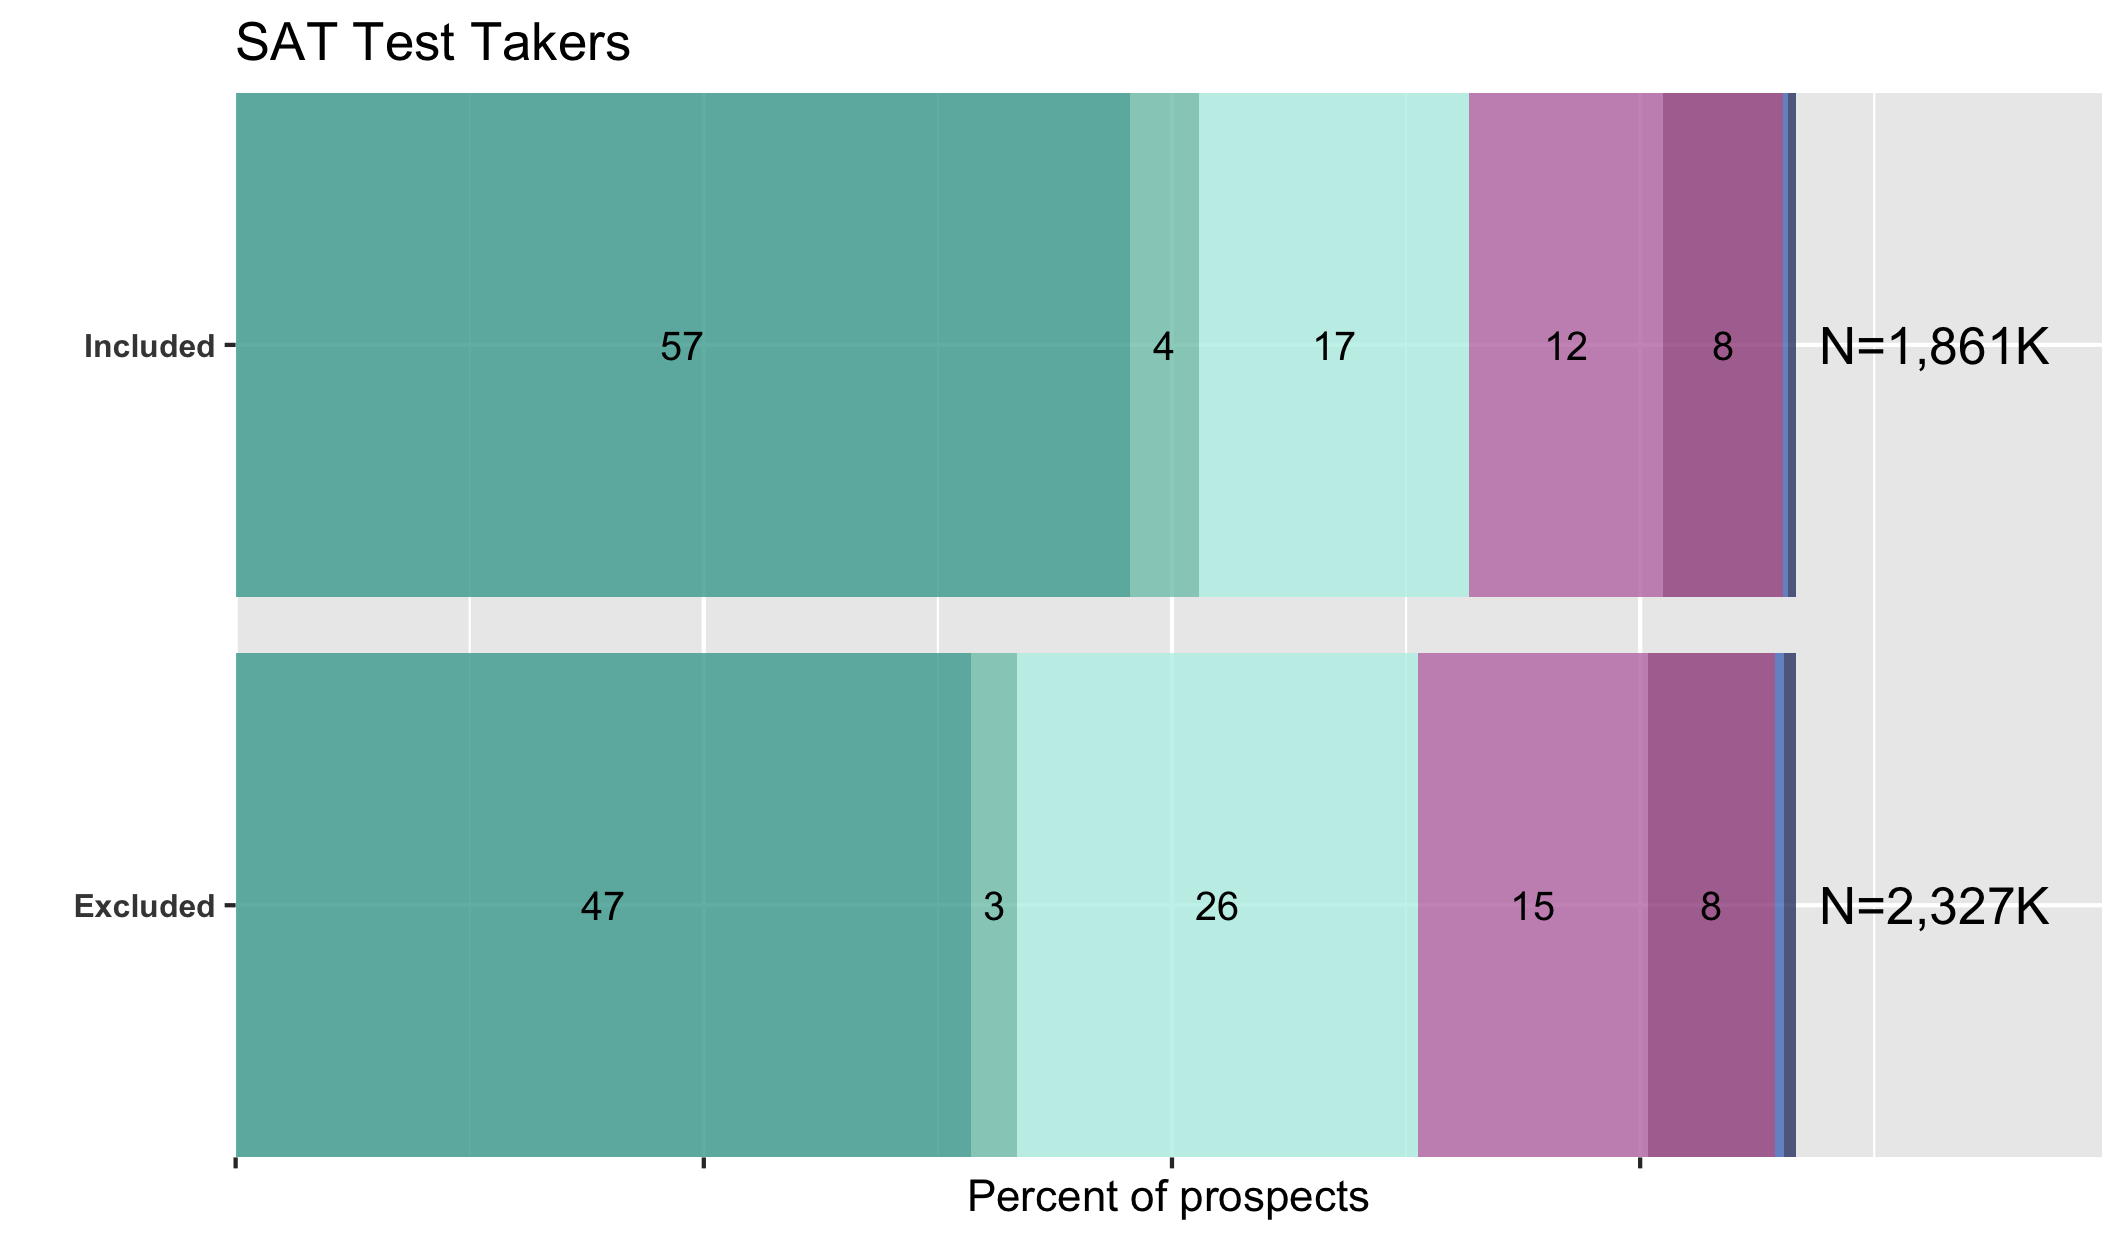
\includegraphics[width=0.4\linewidth]{./../../outputs/figures/p1_sat} 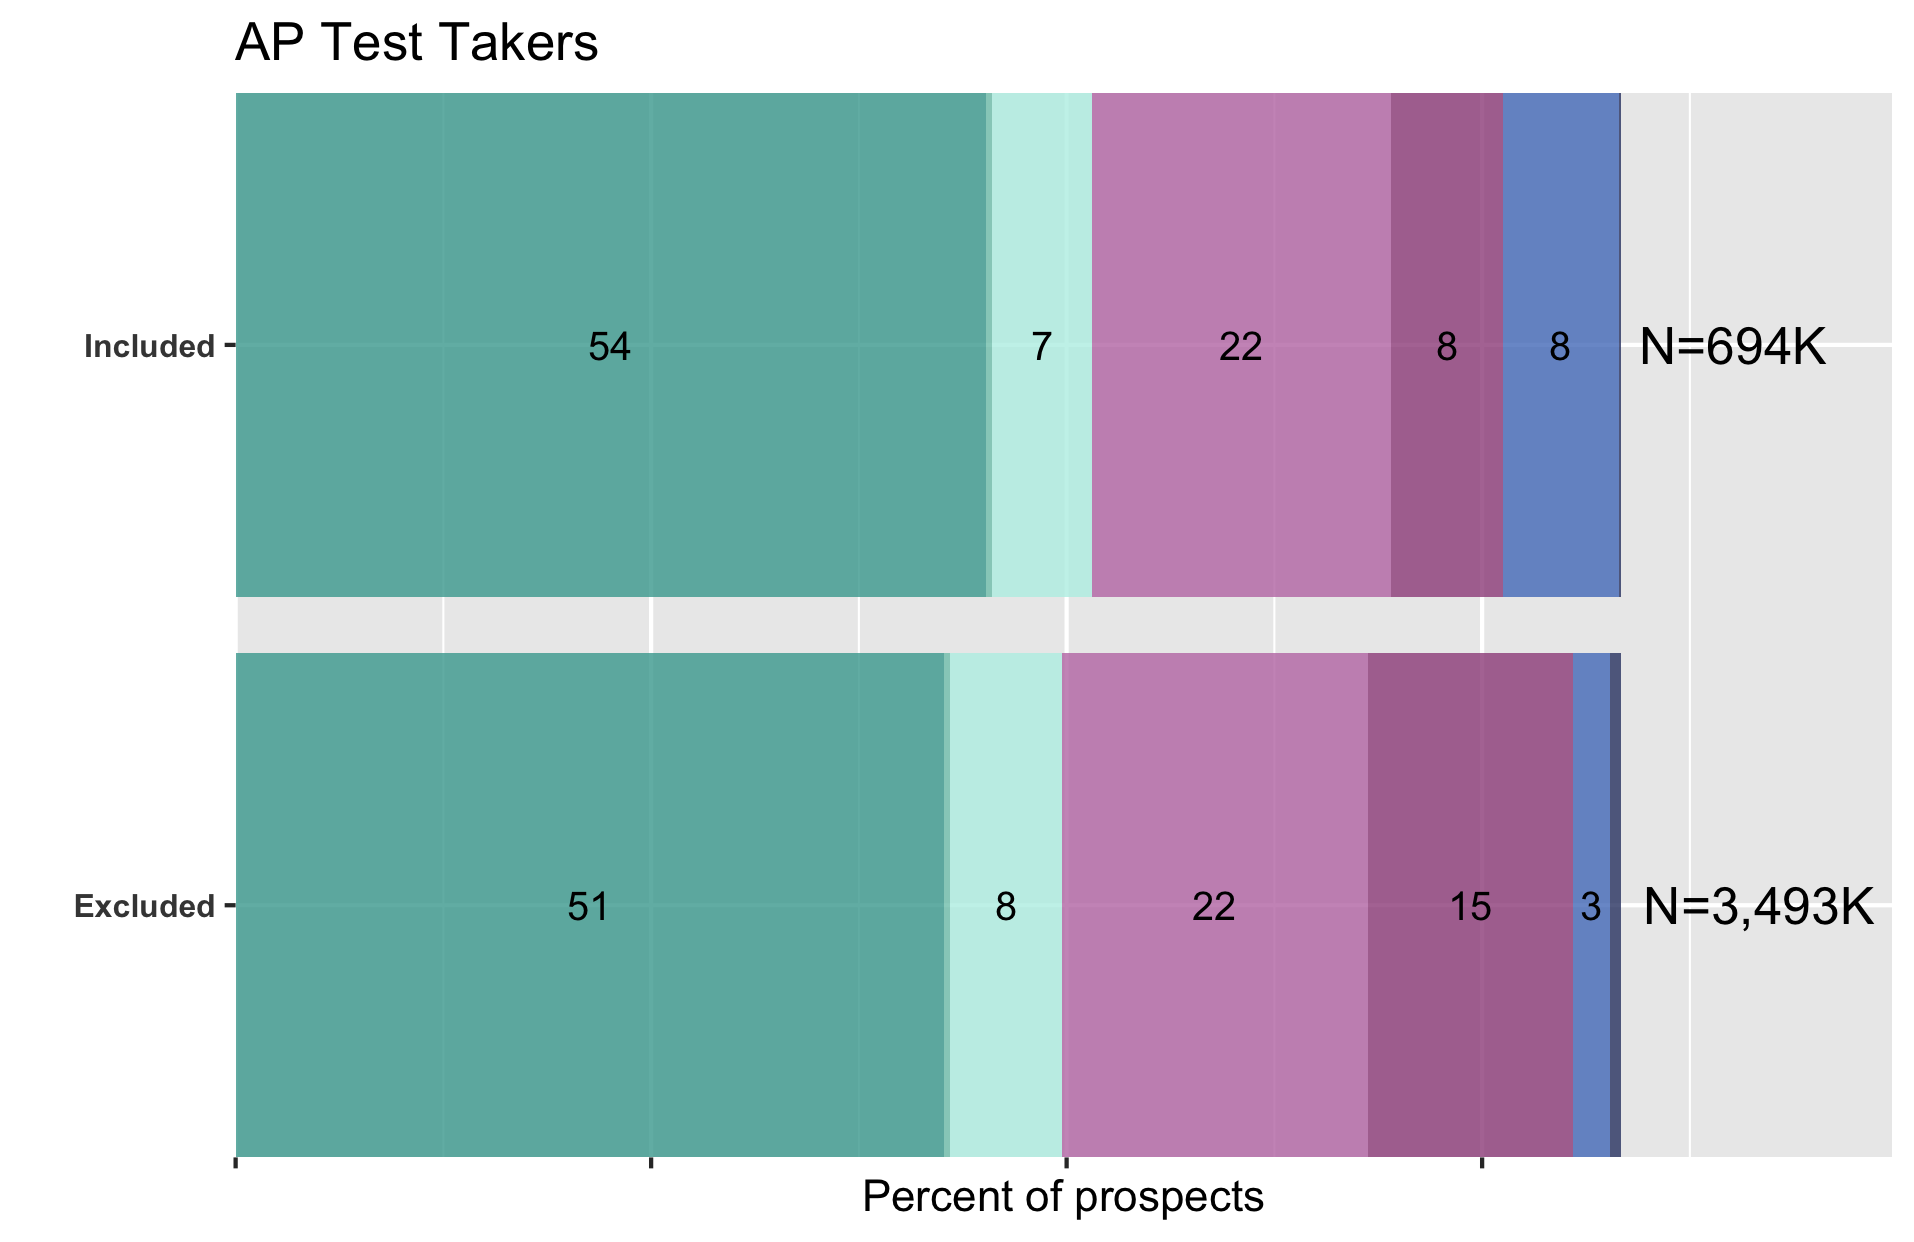
\includegraphics[width=0.4\linewidth]{./../../outputs/figures/p1_ap} 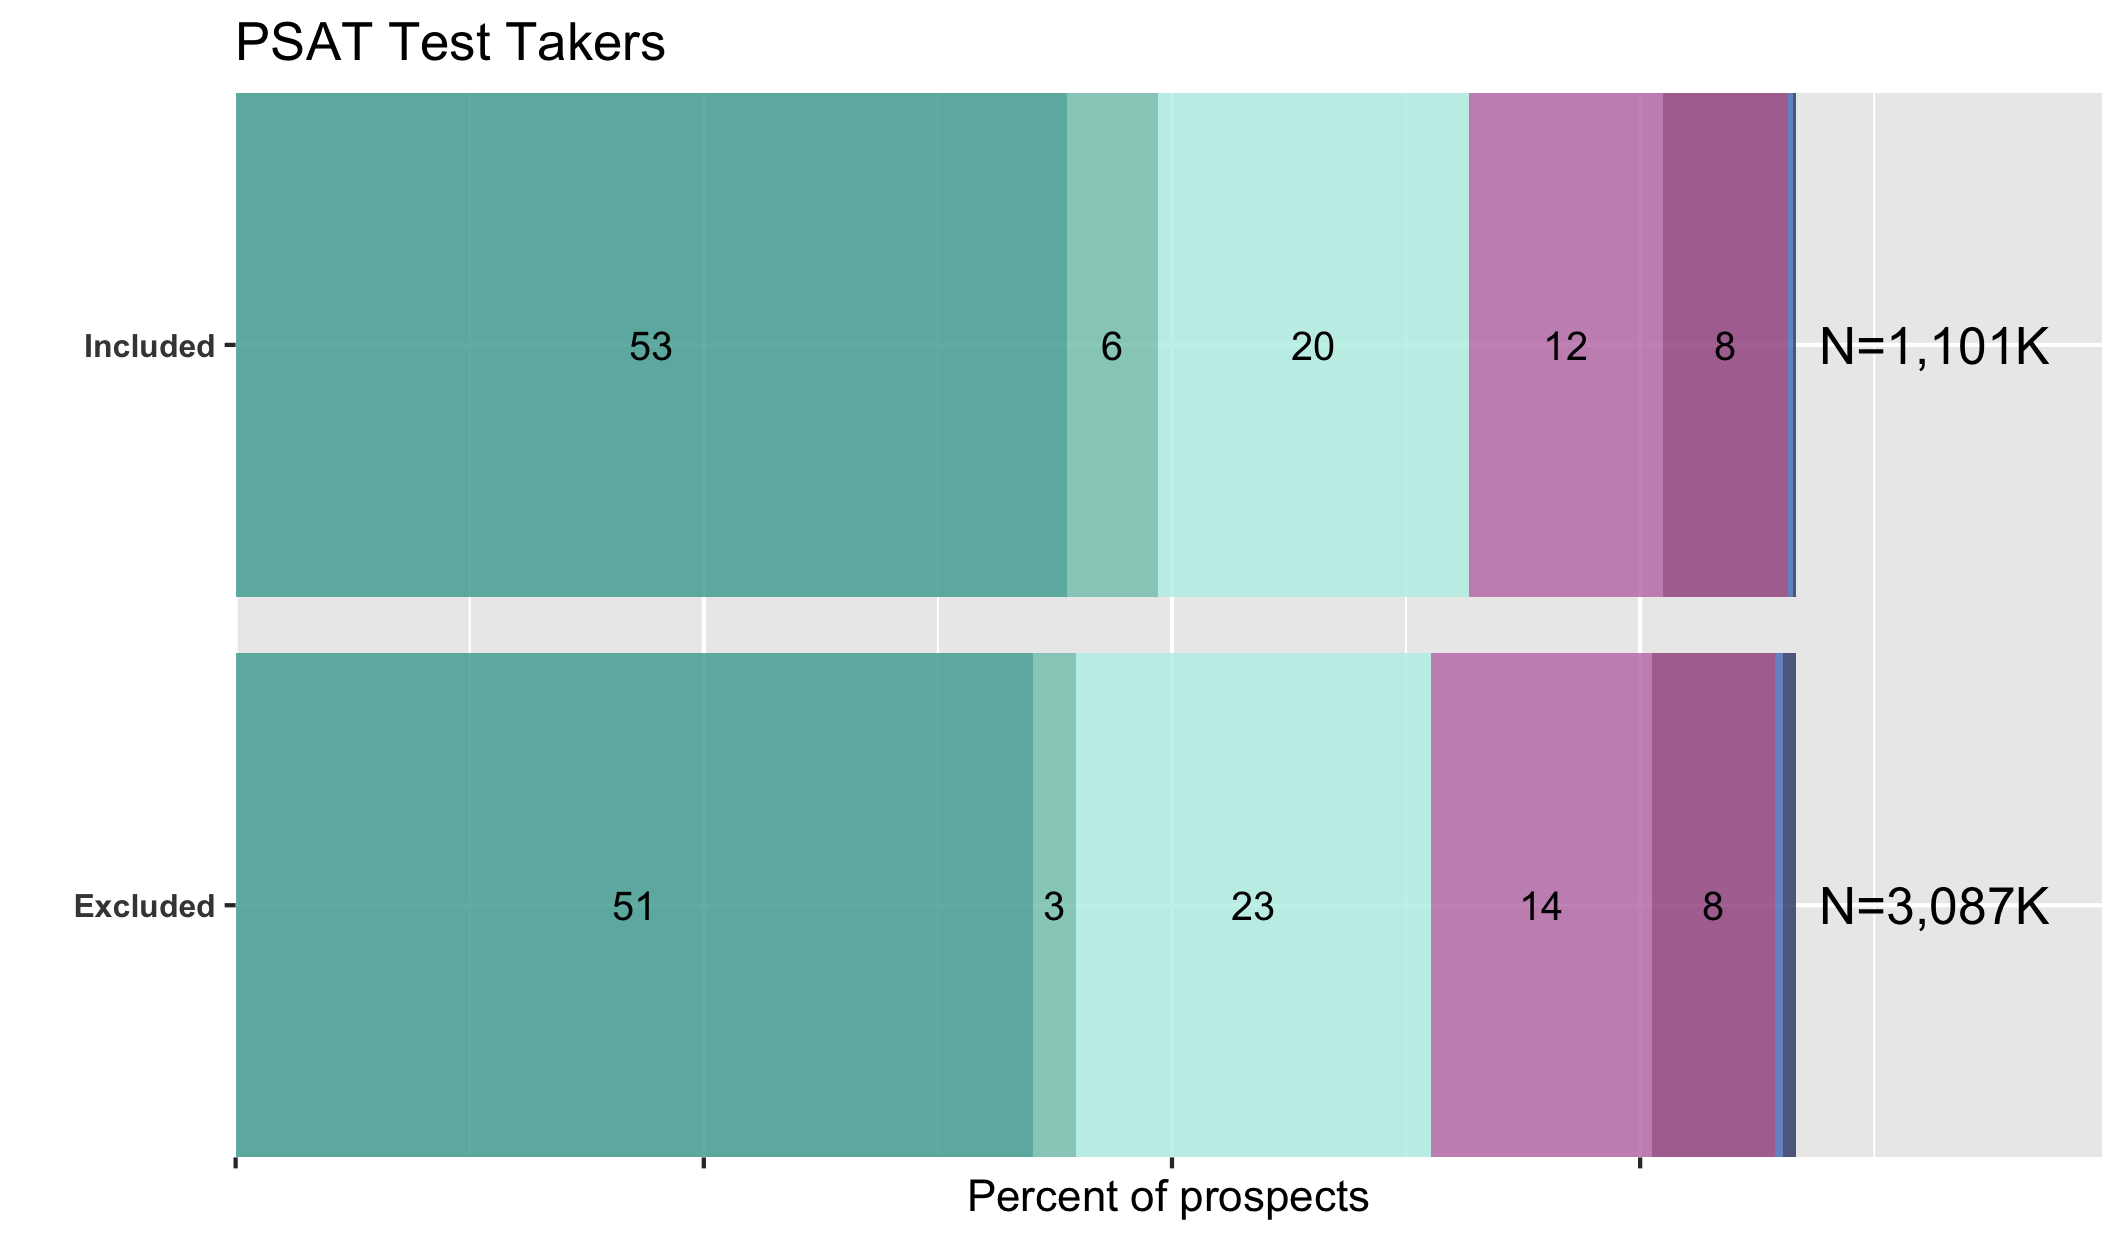
\includegraphics[width=0.4\linewidth]{./../../outputs/figures/p1_psat} 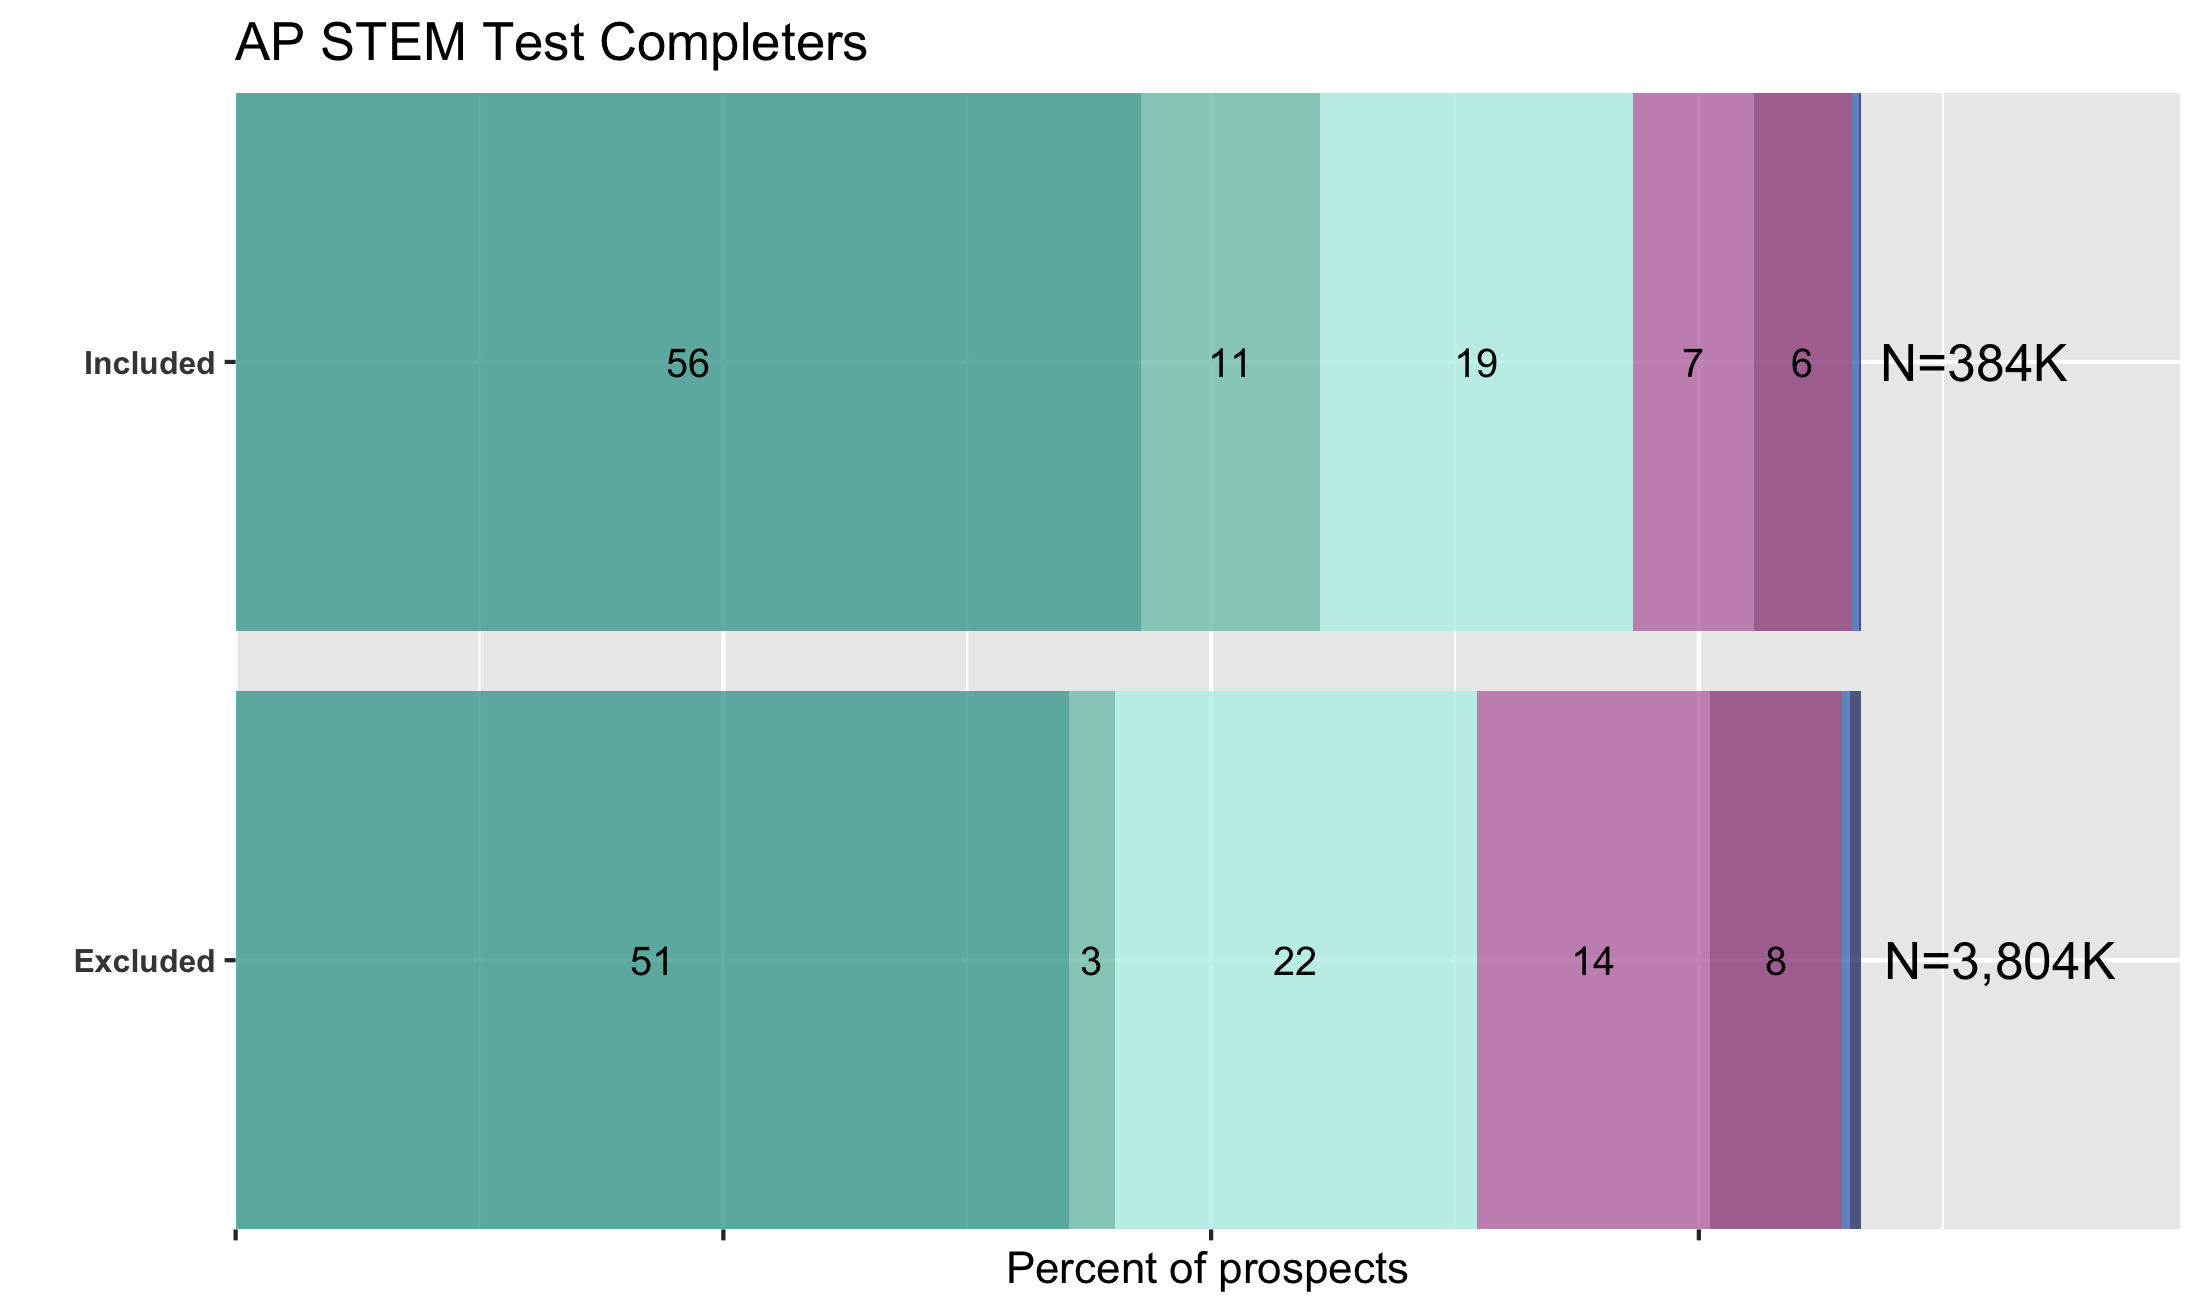
\includegraphics[width=0.4\linewidth]{./../../outputs/figures/p1_apstem} 
\includegraphics[width=0.4\linewidth]{./../../outputs/figures/legend_horizontal} 

}

\caption{Test Takers Across College Extrance, College Pre-Entrance, and AP Assessments}\label{fig:test-takers}
\end{figure}

\begingroup
\fontsize{8}{8}\selectfont
SOURCE: U.S. Department of Education, National Center for Education Statistics, High School Longitudinal Study of 2009 (HSLS09).
\endgroup

\pagebreak



\begin{figure}

{\centering 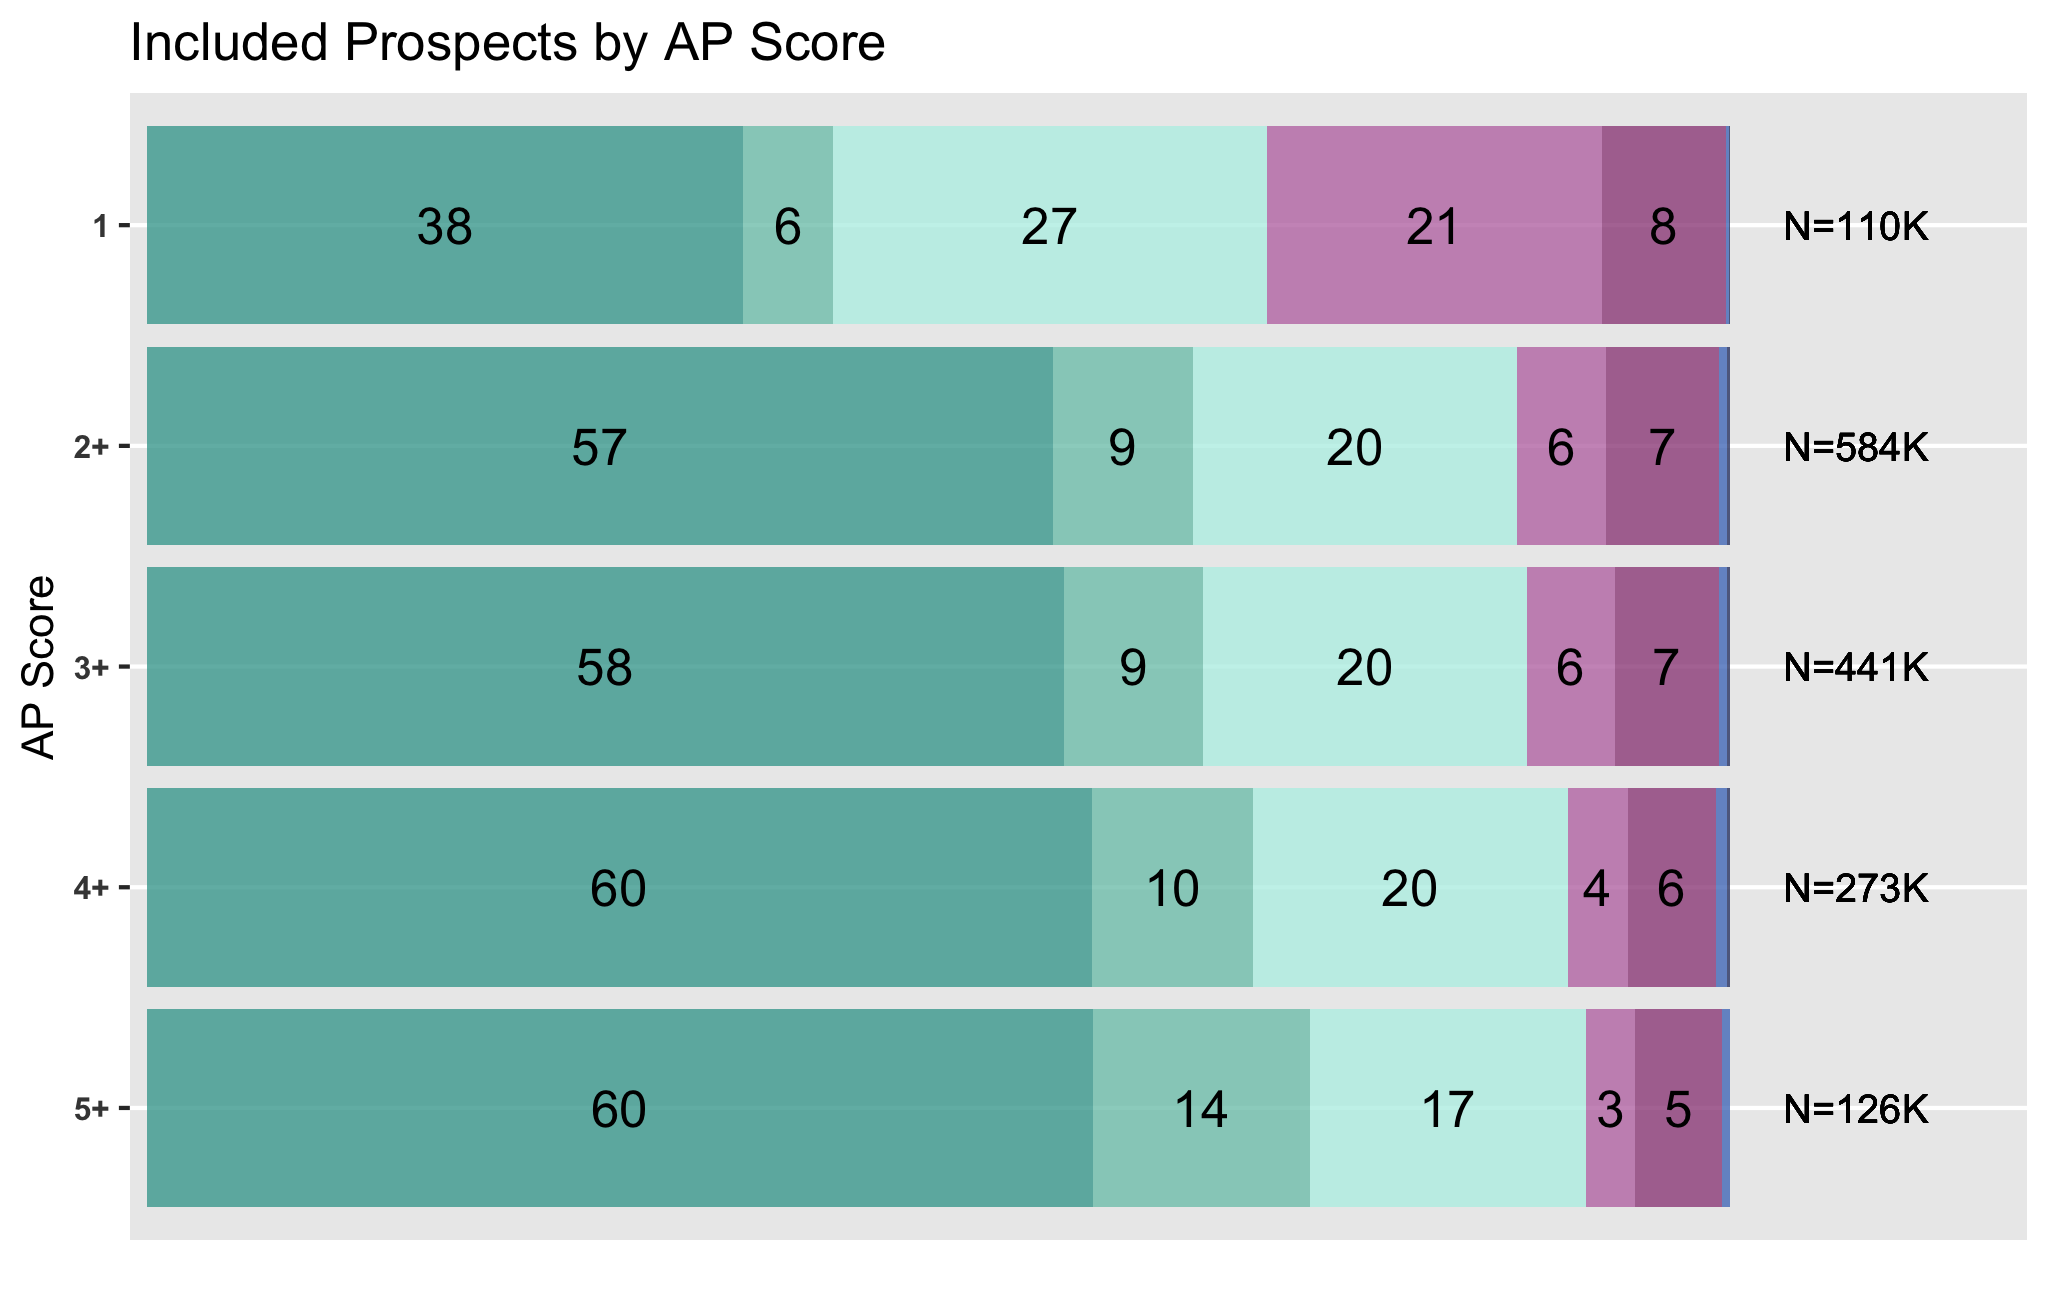
\includegraphics[width=0.37\linewidth]{./../../outputs/figures/p2_ap_incv2} 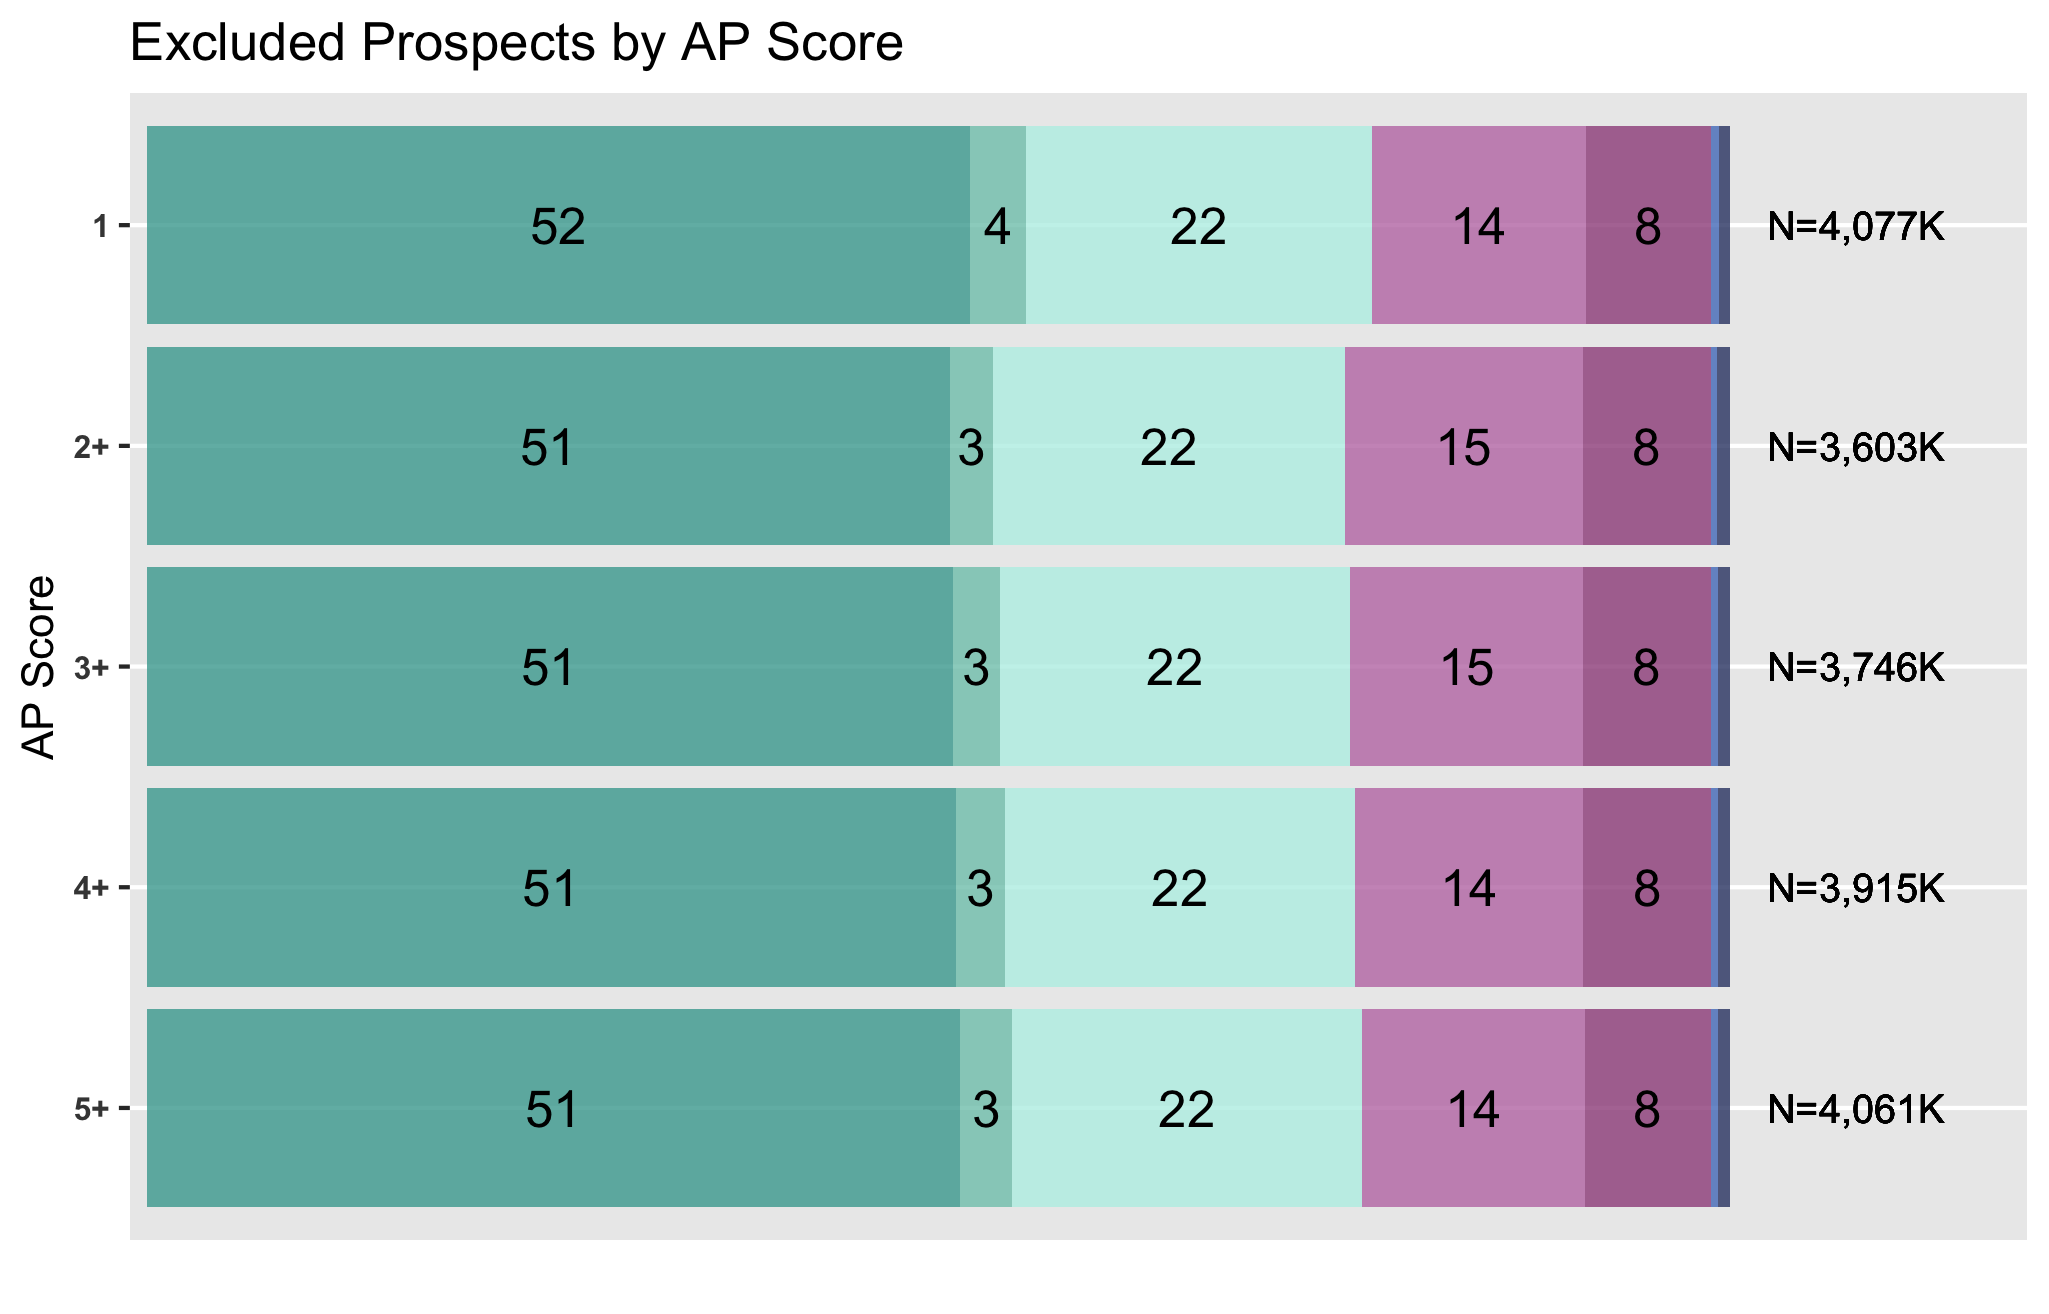
\includegraphics[width=0.37\linewidth]{./../../outputs/figures/p2_ap_excv2} 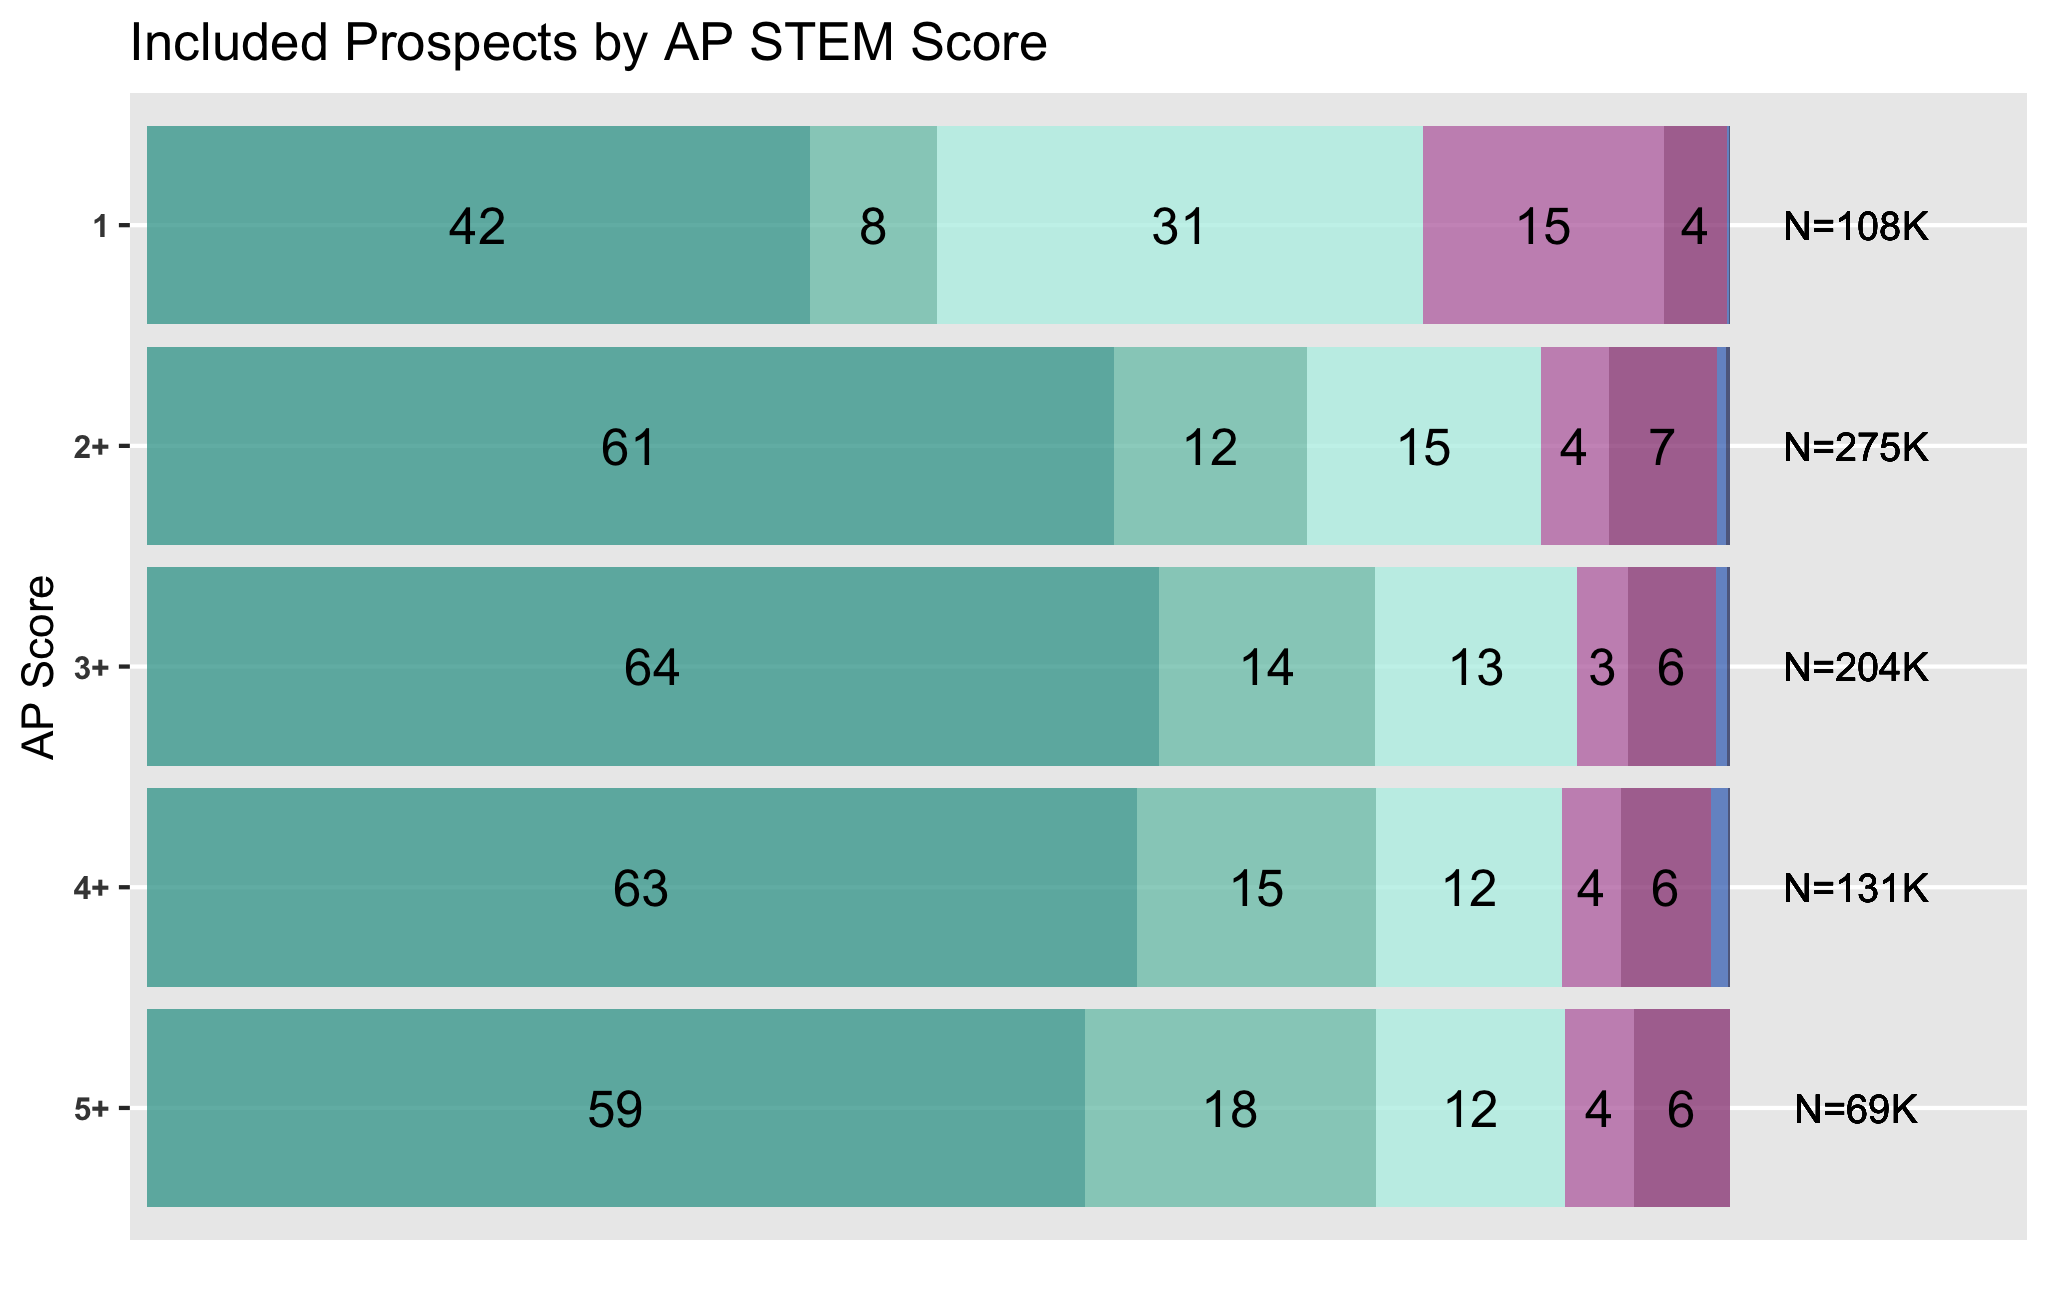
\includegraphics[width=0.37\linewidth]{./../../outputs/figures/p2_apstem_incv2} 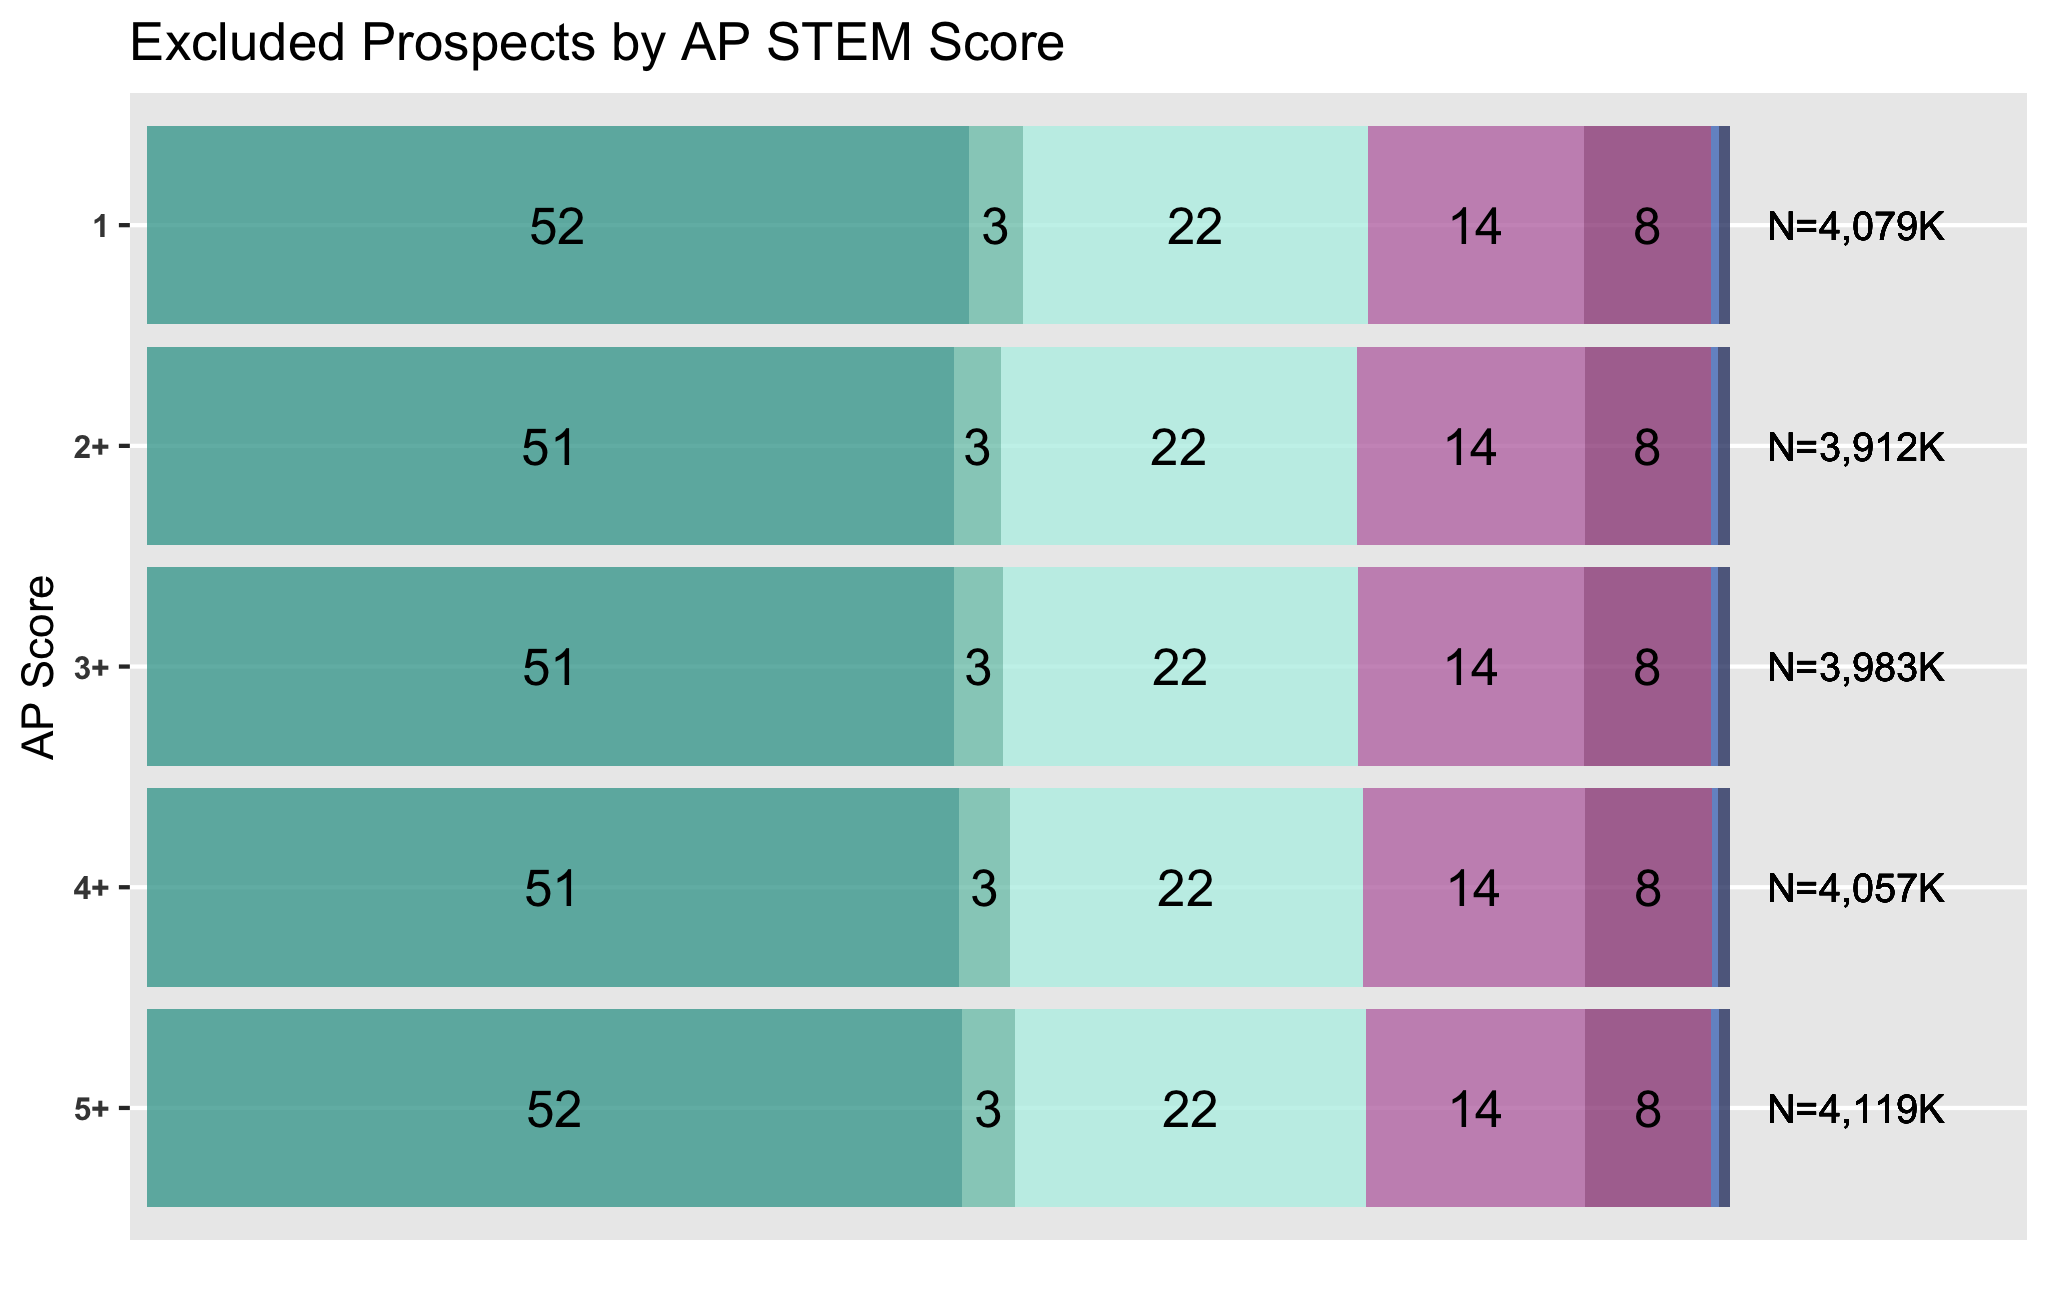
\includegraphics[width=0.37\linewidth]{./../../outputs/figures/p2_apstem_excv2} 
\includegraphics[width=0.37\linewidth]{./../../outputs/figures/legend_horizontal} 

}

\caption{AP Filter Across Thresholds}\label{fig:thresholds-tests-ap}
\end{figure}

\begingroup
\fontsize{8}{8}\selectfont
SOURCE: U.S. Department of Education, National Center for Education Statistics, High School Longitudinal Study of 2009 (HSLS09).
\endgroup

\pagebreak

\end{landscape}

\pagebreak

\begin{figure}
\centering
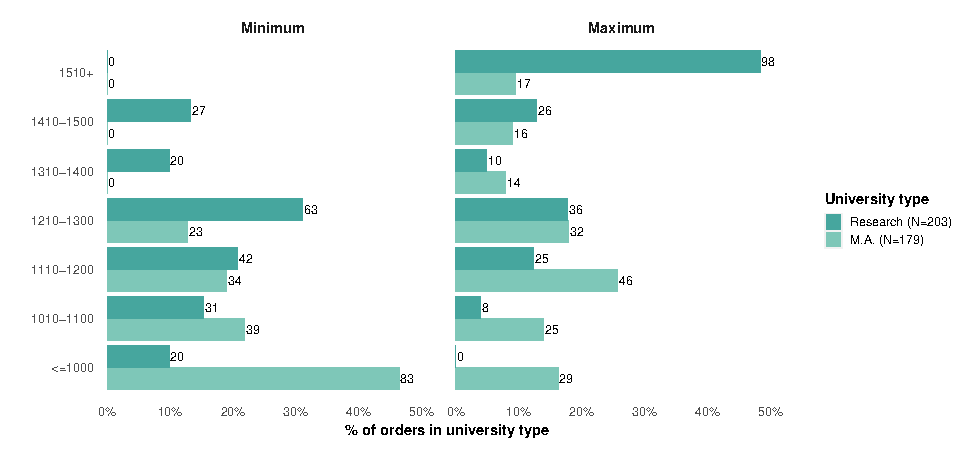
\includegraphics{eepa_student_list_manuscript_c_a_files/figure-latex/orders-psat-1.pdf}
\caption{\label{fig:orders-psat}PSAT Filter Used by Research vs.~Master's Universities}
\end{figure}

\pagebreak

\begin{figure}

{\centering 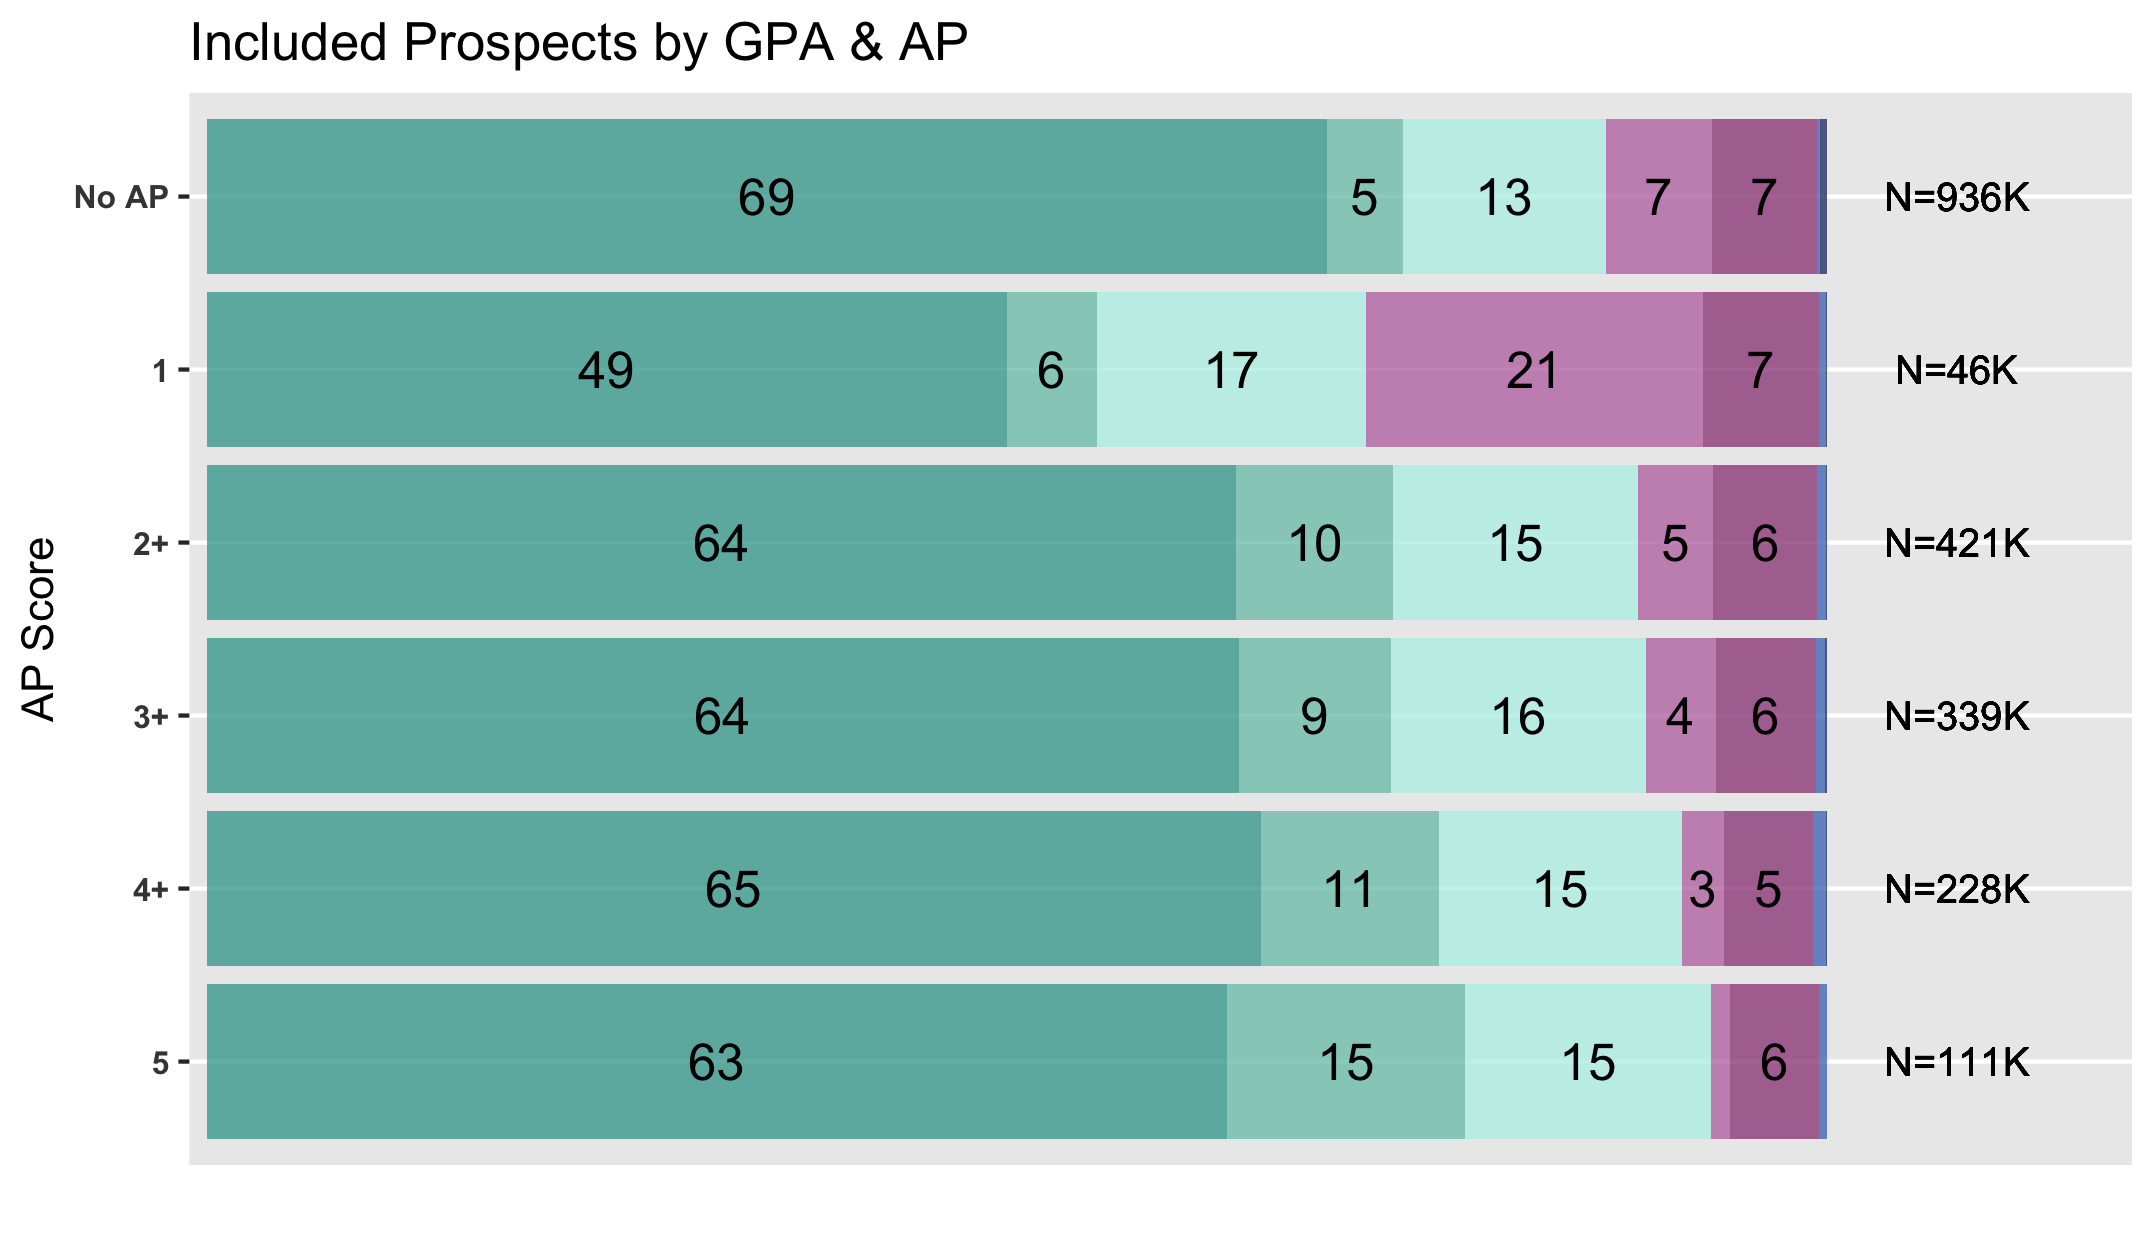
\includegraphics[width=0.8\linewidth]{./../../outputs/figures/combo3_inc_apv2} 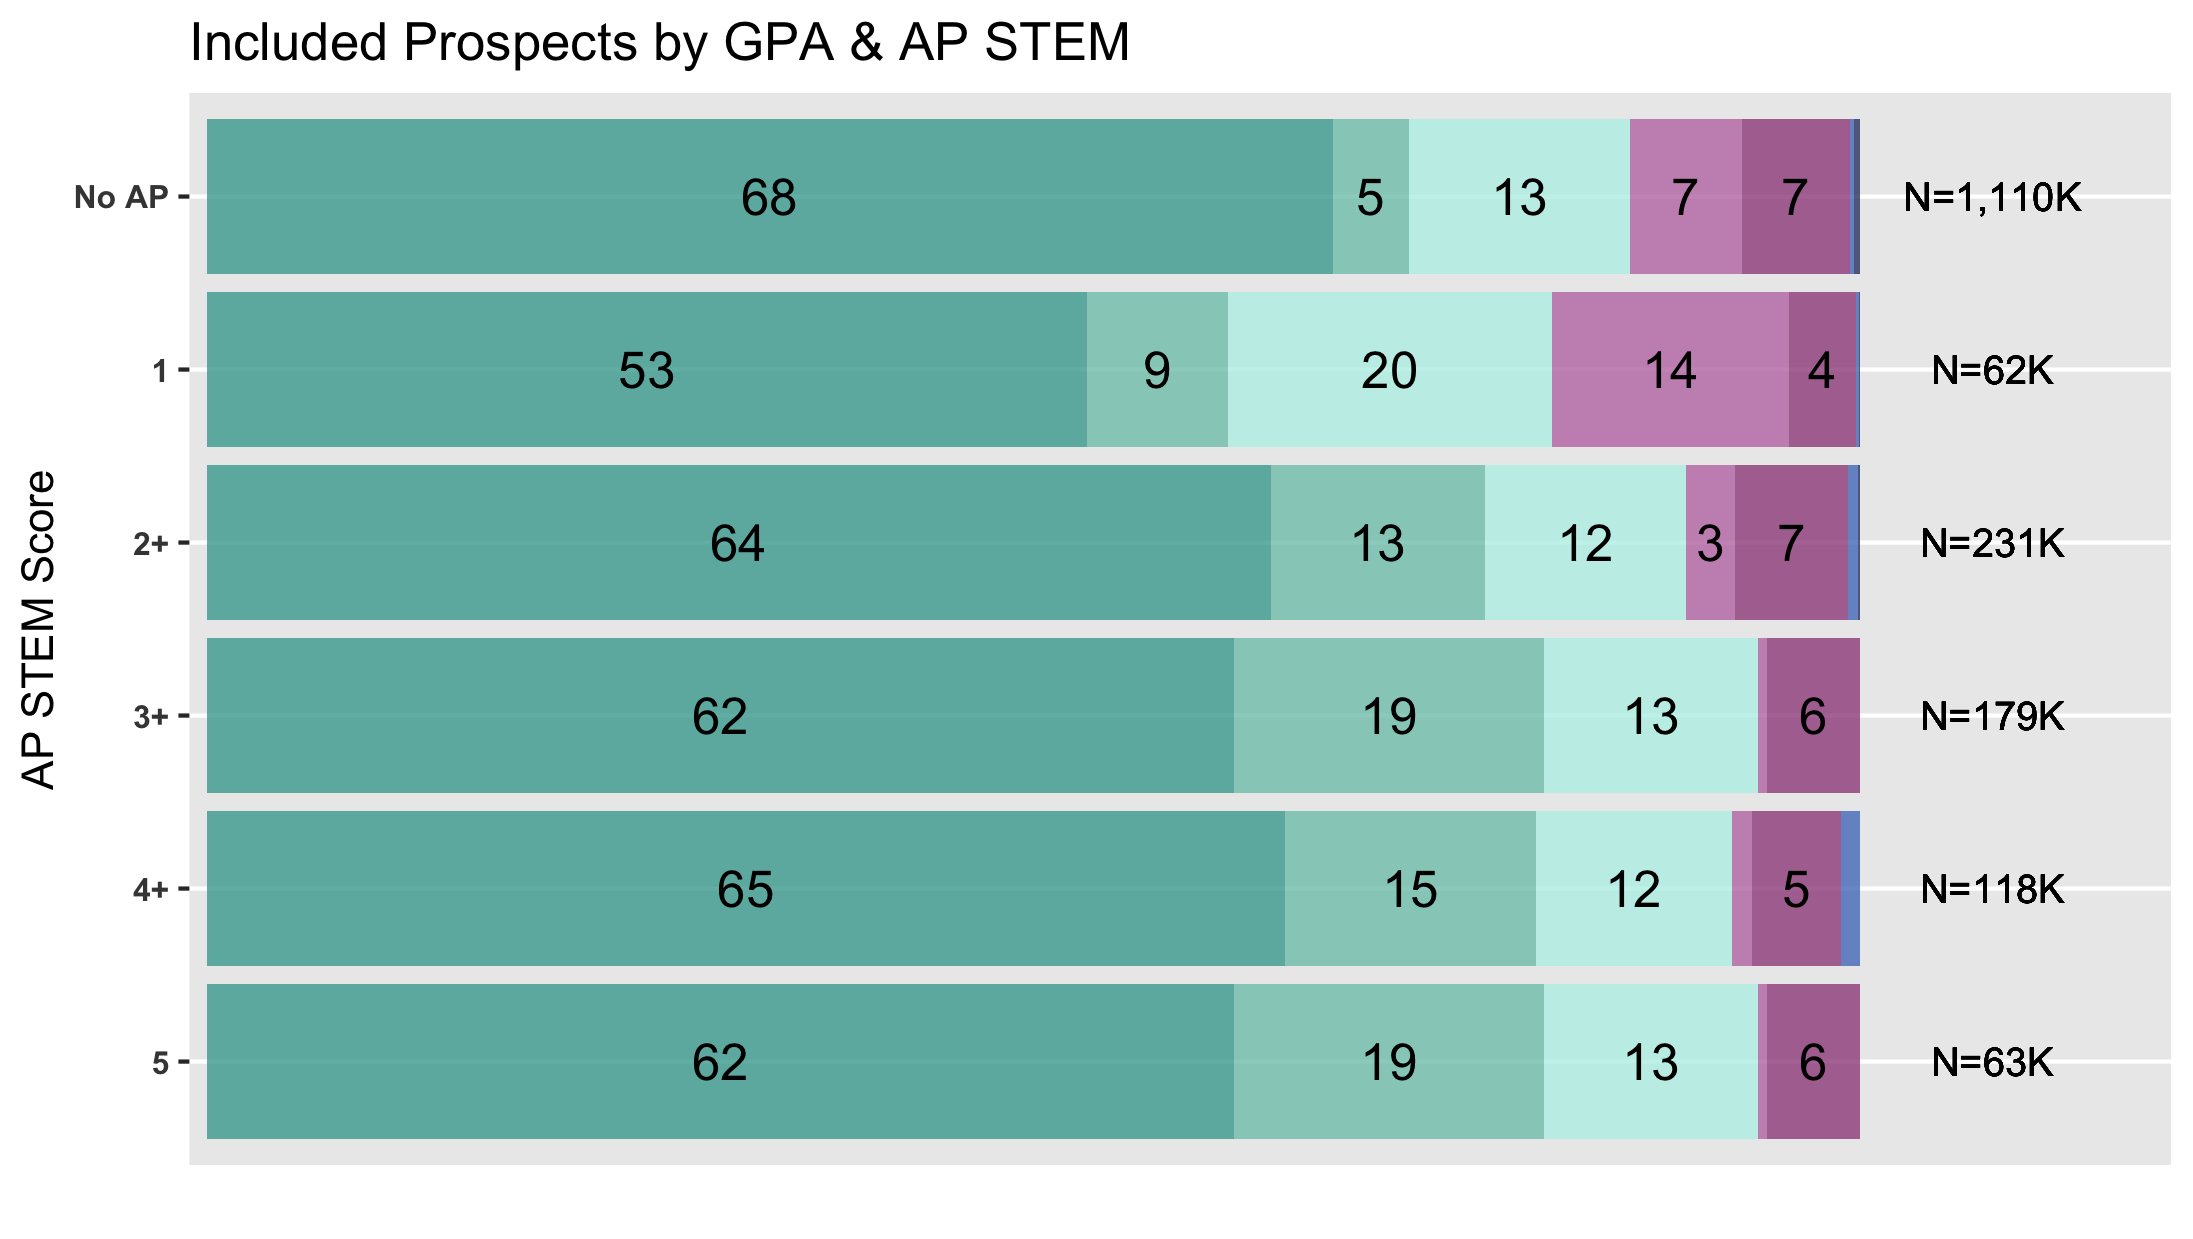
\includegraphics[width=0.8\linewidth]{./../../outputs/figures/combo3_inc_apstemv2} 
\includegraphics[width=0.8\linewidth]{./../../outputs/figures/legend_horizontal} 

}

\caption{Academic Combination: GPA (3.0+) and AP (across score thresholds)}\label{fig:gpa-ap}
\end{figure}

\begingroup
\fontsize{8}{8}\selectfont

SOURCE: U.S. Department of Education, National Center for Education Statistics, High School Longitudinal Study of 2009 (HSLS09).
\endgroup

\pagebreak

\begin{table}[!h]

\caption{\label{tab:descriptives}HSLS09 Descriptive Statistics}
\centering
\resizebox{\linewidth}{!}{
\fontsize{7}{9}\selectfont
\begin{tabular}[t]{lrrrr}
\toprule
\textbf{ } & \textbf{Unweighted} & \textbf{N} & \textbf{SE} & \textbf{Pct}\\
\midrule
\em{\textbf{Race/Ethnicity}} & \em{\textbf{}} & \em{\textbf{}} & \em{\textbf{}} & \em{\textbf{}}\\
White & 9,390 & 2,163,043 & 45,293 & 51.7\\
Asian & 1,370 & 150,222 & 15,373 & 3.6\\
Hisp & 2,520 & 920,384 & 41,451 & 22.0\\
Black & 1,660 & 574,370 & 36,346 & 13.7\\
Multi & 1,410 & 332,043 & 12,921 & 7.9\\
NH/PI & 70 & 18,784 & 5,241 & 0.4\\
AI/AN & 110 & 28,519 & 6,288 & 0.7\\
 &  &  &  & \\
\em{\textbf{Academic Filters}} & \em{\textbf{}} & \em{\textbf{}} & \em{\textbf{}} & \em{\textbf{}}\\
College Entrance Exam Completer & 7,910 & 1,860,677 & 54,277 & 55.6\\
College Pre-Entrance Exam Completer & 4,780 & 3,086,739 & 51,247 & 73.7\\
AP test-taker (any) & 2,990 & 694,359 & 33,918 & 16.6\\
AP test-taker (STEM) & 1,800 & 383,669 & 23,721 & 9.2\\
Academic GPA & 16,480 & 4,177,402 & 6,863 & 99.8\\
Missing Academic GPA & 40 & 9,964 & 6,562 & 0.2\\
\bottomrule
\end{tabular}}
\end{table}
\begingroup\fontsize{8}{12}\selectfont

\emph{NOTE: Unweighted sample sizes rounded to nearest 10 per NCES restricted data license regulations.}

\emph{SOURCE: U.S. Department of Education, National Center for Education
Statistics, High School Longitudinal Study of 2009 (HSLS09).}

\pagebreak
\landscape

\begin{table}[!h]

\caption{\label{tab:sampletable}Characteristics of universities in public records request sample}
\centering
\resizebox{\linewidth}{!}{
\fontsize{3}{5}\selectfont
\begin{tabular}[t]{lrrrrrrrrrrr}
\toprule
\multicolumn{4}{c}{ } & \multicolumn{7}{c}{Undergraduate Freshmen} \\
\cmidrule(l{3pt}r{3pt}){5-11}
\begingroup\fontsize{2}{4}\selectfont \textbf{ }\endgroup & \begingroup\fontsize{2}{4}\selectfont \textbf{Type}\endgroup & \begingroup\fontsize{2}{4}\selectfont \textbf{Tuition \& Fees, In-State}\endgroup & \begingroup\fontsize{2}{4}\selectfont \textbf{Total Enrollment}\endgroup & \begingroup\fontsize{2}{4}\selectfont \textbf{\% Non-Resident}\endgroup & \begingroup\fontsize{2}{4}\selectfont \textbf{\% Pell}\endgroup & \begingroup\fontsize{2}{4}\selectfont \textbf{\% Asian}\endgroup & \begingroup\fontsize{2}{4}\selectfont \textbf{\% Black}\endgroup & \begingroup\fontsize{2}{4}\selectfont \textbf{\% Hispanic}\endgroup & \begingroup\fontsize{2}{4}\selectfont \textbf{\% Native American}\endgroup & \begingroup\fontsize{2}{4}\selectfont \textbf{\% Multiracial}\endgroup & \begingroup\fontsize{2}{4}\selectfont \textbf{\% White}\endgroup\\
\midrule
\cellcolor{gray!6}{Arizona State University-Tempe} & \cellcolor{gray!6}{Research} & \cellcolor{gray!6}{\$10,792} & \cellcolor{gray!6}{54,161} & \cellcolor{gray!6}{40} & \cellcolor{gray!6}{29} & \cellcolor{gray!6}{9} & \cellcolor{gray!6}{4} & \cellcolor{gray!6}{23} & \cellcolor{gray!6}{1} & \cellcolor{gray!6}{5} & \cellcolor{gray!6}{50}\\
Northern Arizona University & Research & \$10,289 & 29,609 & 38 & 35 & 2 & 3 & 26 & 2 & 7 & 57\\
\cellcolor{gray!6}{University of California-Davis} & \cellcolor{gray!6}{Research} & \cellcolor{gray!6}{\$14,419} & \cellcolor{gray!6}{31,437} & \cellcolor{gray!6}{19} & \cellcolor{gray!6}{33} & \cellcolor{gray!6}{25} & \cellcolor{gray!6}{2} & \cellcolor{gray!6}{23} & \cellcolor{gray!6}{0} & \cellcolor{gray!6}{5} & \cellcolor{gray!6}{21}\\
University of California-Irvine & Research & \$13,738 & 28,947 & 26 & 38 & 38 & 2 & 26 & 0 & 4 & 11\\
\cellcolor{gray!6}{University of California-San Diego} & \cellcolor{gray!6}{Research} & \cellcolor{gray!6}{\$14,018} & \cellcolor{gray!6}{29,613} & \cellcolor{gray!6}{26} & \cellcolor{gray!6}{31} & \cellcolor{gray!6}{34} & \cellcolor{gray!6}{1} & \cellcolor{gray!6}{23} & \cellcolor{gray!6}{0} & \cellcolor{gray!6}{5} & \cellcolor{gray!6}{18}\\
University of Illinois at Chicago & Research & \$15,027 & 19,476 & 8 & 59 & 22 & 8 & 40 & 0 & 3 & 22\\
\cellcolor{gray!6}{University of Illinois at Urbana-Champaign} & \cellcolor{gray!6}{Research} & \cellcolor{gray!6}{\$17,293} & \cellcolor{gray!6}{35,476} & \cellcolor{gray!6}{26} & \cellcolor{gray!6}{24} & \cellcolor{gray!6}{20} & \cellcolor{gray!6}{7} & \cellcolor{gray!6}{13} & \cellcolor{gray!6}{0} & \cellcolor{gray!6}{3} & \cellcolor{gray!6}{41}\\
Illinois State University & Research & \$12,353 & 20,115 & 4 & 30 & 2 & 10 & 12 & 0 & 3 & 71\\
\cellcolor{gray!6}{Northeastern Illinois University} & \cellcolor{gray!6}{Master's} & \cellcolor{gray!6}{\$9,638} & \cellcolor{gray!6}{9,260} & \cellcolor{gray!6}{2} & \cellcolor{gray!6}{64} & \cellcolor{gray!6}{6} & \cellcolor{gray!6}{30} & \cellcolor{gray!6}{44} & \cellcolor{gray!6}{0} & \cellcolor{gray!6}{2} & \cellcolor{gray!6}{11}\\
University of Illinois at Springfield & Master's & \$11,523 & 3,500 & 10 & 38 & 2 & 18 & 18 & 1 & 5 & 52\\
\cellcolor{gray!6}{Texas A\&M University-Texarkana} & \cellcolor{gray!6}{Master's} & \cellcolor{gray!6}{\$6,963} & \cellcolor{gray!6}{1,953} & \cellcolor{gray!6}{16} & \cellcolor{gray!6}{42} & \cellcolor{gray!6}{1} & \cellcolor{gray!6}{16} & \cellcolor{gray!6}{23} & \cellcolor{gray!6}{0} & \cellcolor{gray!6}{4} & \cellcolor{gray!6}{46}\\
Stephen F Austin State University & Master's & \$7,716 & 12,149 & 1 & 41 & 1 & 16 & 24 & 0 & 5 & 53\\
\cellcolor{gray!6}{Tarleton State University} & \cellcolor{gray!6}{Master's} & \cellcolor{gray!6}{\$7,367} & \cellcolor{gray!6}{12,853} & \cellcolor{gray!6}{2} & \cellcolor{gray!6}{40} & \cellcolor{gray!6}{1} & \cellcolor{gray!6}{6} & \cellcolor{gray!6}{21} & \cellcolor{gray!6}{0} & \cellcolor{gray!6}{3} & \cellcolor{gray!6}{67}\\
Texas A \& M University-College Station & Research & \$10,294 & 53,515 & 6 & 21 & 9 & 3 & 26 & 0 & 3 & 58\\
\bottomrule
\end{tabular}}
\end{table}
\begingroup
\fontsize{10}{10}\selectfont

\emph{SOURCE: U.S. Department of Education, Integrated Postsecondary Education Data System, 2017-18.}
\endgroup

\pagebreak
\endlandscape

\begin{table}[!h]

\caption{\label{tab:p1table}Assessment Completer Differences in Proportion}
\centering
\resizebox{\linewidth}{!}{
\fontsize{2.5}{4.5}\selectfont
\begin{tabular}[t]{lrrrrr}
\toprule
\begingroup\fontsize{2}{4}\selectfont \textbf{ }\endgroup & \begingroup\fontsize{2}{4}\selectfont \textbf{Included}\endgroup & \begingroup\fontsize{2}{4}\selectfont \textbf{Excluded}\endgroup & \begingroup\fontsize{2}{4}\selectfont \textbf{Difference}\endgroup & \begingroup\fontsize{2}{4}\selectfont \textbf{Lower CI}\endgroup & \begingroup\fontsize{2}{4}\selectfont \textbf{Upper CI}\endgroup\\
\midrule
\addlinespace[0.3em]
\multicolumn{6}{l}{\textbf{College Entrance Exam}}\\
\cellcolor{gray!6}{\hspace{1em}White} & \cellcolor{gray!6}{0.573} & \cellcolor{gray!6}{0.472} & \cellcolor{gray!6}{0.101***} & \cellcolor{gray!6}{0.100} & \cellcolor{gray!6}{0.102}\\
\hspace{1em}Asian & 0.045 & 0.029 & 0.016*** & 0.015 & 0.016\\
\cellcolor{gray!6}{\hspace{1em}Hisp} & \cellcolor{gray!6}{0.173} & \cellcolor{gray!6}{0.257} & \cellcolor{gray!6}{-0.084***} & \cellcolor{gray!6}{-0.085} & \cellcolor{gray!6}{-0.083}\\
\hspace{1em}Black & 0.124 & 0.147 & -0.023*** & -0.024 & -0.022\\
\cellcolor{gray!6}{\hspace{1em}Multi} & \cellcolor{gray!6}{0.077} & \cellcolor{gray!6}{0.081} & \cellcolor{gray!6}{-0.004***} & \cellcolor{gray!6}{-0.005} & \cellcolor{gray!6}{-0.004}\\
\hspace{1em}NH/PI & 0.003 & 0.006 & -0.003*** & -0.003 & -0.002\\
\cellcolor{gray!6}{\hspace{1em}AI/AN} & \cellcolor{gray!6}{0.005} & \cellcolor{gray!6}{0.008} & \cellcolor{gray!6}{-0.003***} & \cellcolor{gray!6}{-0.003} & \cellcolor{gray!6}{-0.003}\\
\addlinespace[0.3em]
\multicolumn{6}{l}{\textbf{College Pre-Entrance Exam}}\\
\hspace{1em}White & 0.533 & 0.511 & 0.022*** & 0.021 & 0.023\\
\cellcolor{gray!6}{\hspace{1em}Asian} & \cellcolor{gray!6}{0.058} & \cellcolor{gray!6}{0.028} & \cellcolor{gray!6}{0.030***} & \cellcolor{gray!6}{0.030} & \cellcolor{gray!6}{0.031}\\
\hspace{1em}Hisp & 0.199 & 0.227 & -0.028*** & -0.029 & -0.027\\
\cellcolor{gray!6}{\hspace{1em}Black} & \cellcolor{gray!6}{0.125} & \cellcolor{gray!6}{0.142} & \cellcolor{gray!6}{-0.017***} & \cellcolor{gray!6}{-0.018} & \cellcolor{gray!6}{-0.016}\\
\hspace{1em}Multi & 0.08 & 0.079 & 0.001*** & 0.001 & 0.002\\
\cellcolor{gray!6}{\hspace{1em}NH/PI} & \cellcolor{gray!6}{0.003} & \cellcolor{gray!6}{0.005} & \cellcolor{gray!6}{-0.002***} & \cellcolor{gray!6}{-0.002} & \cellcolor{gray!6}{-0.002}\\
\hspace{1em}AI/AN & 0.002 & 0.009 & -0.007*** & -0.007 & -0.007\\
\addlinespace[0.3em]
\multicolumn{6}{l}{\textbf{AP}}\\
\cellcolor{gray!6}{\hspace{1em}White} & \cellcolor{gray!6}{0.542} & \cellcolor{gray!6}{0.512} & \cellcolor{gray!6}{0.030***} & \cellcolor{gray!6}{0.029} & \cellcolor{gray!6}{0.031}\\
\hspace{1em}Asian & 0.083 & 0.026 & 0.057*** & 0.056 & 0.058\\
\cellcolor{gray!6}{\hspace{1em}Hisp} & \cellcolor{gray!6}{0.216} & \cellcolor{gray!6}{0.221} & \cellcolor{gray!6}{-0.005***} & \cellcolor{gray!6}{-0.006} & \cellcolor{gray!6}{-0.004}\\
\hspace{1em}Black & 0.081 & 0.148 & -0.067*** & -0.068 & -0.067\\
\cellcolor{gray!6}{\hspace{1em}Multi} & \cellcolor{gray!6}{0.072} & \cellcolor{gray!6}{0.081} & \cellcolor{gray!6}{-0.009***} & \cellcolor{gray!6}{-0.009} & \cellcolor{gray!6}{-0.008}\\
\hspace{1em}NH/PI & 0.005 & 0.004 & 0.001*** & 0.000 & 0.001\\
\cellcolor{gray!6}{\hspace{1em}AI/AN} & \cellcolor{gray!6}{0.001} & \cellcolor{gray!6}{0.008} & \cellcolor{gray!6}{-0.007***} & \cellcolor{gray!6}{-0.007} & \cellcolor{gray!6}{-0.006}\\
\addlinespace[0.3em]
\multicolumn{6}{l}{\textbf{AP STEM}}\\
\hspace{1em}White & 0.557 & 0.513 & 0.044*** & 0.043 & 0.046\\
\cellcolor{gray!6}{\hspace{1em}Asian} & \cellcolor{gray!6}{0.11} & \cellcolor{gray!6}{0.028} & \cellcolor{gray!6}{0.082***} & \cellcolor{gray!6}{0.081} & \cellcolor{gray!6}{0.083}\\
\hspace{1em}Hisp & 0.193 & 0.223 & -0.030*** & -0.031 & -0.029\\
\cellcolor{gray!6}{\hspace{1em}Black} & \cellcolor{gray!6}{0.074} & \cellcolor{gray!6}{0.144} & \cellcolor{gray!6}{-0.070***} & \cellcolor{gray!6}{-0.071} & \cellcolor{gray!6}{-0.069}\\
\hspace{1em}Multi & 0.06 & 0.081 & -0.021*** & -0.022 & -0.020\\
\cellcolor{gray!6}{\hspace{1em}NH/PI} & \cellcolor{gray!6}{0.004} & \cellcolor{gray!6}{0.005} & \cellcolor{gray!6}{-0.001} & \cellcolor{gray!6}{-0.000} & \cellcolor{gray!6}{0.000}\\
\hspace{1em}AI/AN & 0.002 & 0.007 & -0.005*** & -0.006 & -0.005\\
\bottomrule
\end{tabular}}
\end{table}
\begingroup
\fontsize{10}{10}\selectfont

\emph{NOTE: \texttt{*}p\textless0.05, \texttt{**}p\textless0.01, \texttt{***}p\textless0.001}

\emph{SOURCE: U.S. Department of Education, National Center for Education Statistics, High School Longitudinal Study of 2009 (HSLS09).}
\endgroup

\pagebreak

\begin{table}[!h]

\caption{\label{tab:p2table}Score Threshold Proportion Differences in Included vs. Excluded across Race/Ethnicity}
\centering
\resizebox{\linewidth}{!}{
\fontsize{4}{6}\selectfont
\begin{tabular}[t]{lrrrrrrr}
\toprule
\begingroup\fontsize{6}{8}\selectfont \textbf{ }\endgroup & \begingroup\fontsize{6}{8}\selectfont \textbf{White}\endgroup & \begingroup\fontsize{6}{8}\selectfont \textbf{Asian}\endgroup & \begingroup\fontsize{6}{8}\selectfont \textbf{Hisp}\endgroup & \begingroup\fontsize{6}{8}\selectfont \textbf{Black}\endgroup & \begingroup\fontsize{6}{8}\selectfont \textbf{Multi}\endgroup & \begingroup\fontsize{6}{8}\selectfont \textbf{NH/PI}\endgroup & \begingroup\fontsize{6}{8}\selectfont \textbf{AI/AN}\endgroup\\
\midrule
\addlinespace[0.3em]
\multicolumn{8}{l}{\textbf{College Entrance Exam}}\\
\cellcolor{gray!6}{\hspace{1em}Less than 1000} & \cellcolor{gray!6}{-0.062***} & \cellcolor{gray!6}{-0.010***} & \cellcolor{gray!6}{0.004***} & \cellcolor{gray!6}{0.065***} & \cellcolor{gray!6}{0.005***} & \cellcolor{gray!6}{-0.003***} & \cellcolor{gray!6}{0.002***}\\
\hspace{1em}1000+ & 0.217*** & 0.033*** & -0.129*** & -0.103*** & -0.012*** & -0.001*** & -0.006***\\
\cellcolor{gray!6}{\hspace{1em}1200+} & \cellcolor{gray!6}{0.209***} & \cellcolor{gray!6}{0.057***} & \cellcolor{gray!6}{-0.137***} & \cellcolor{gray!6}{-0.103***} & \cellcolor{gray!6}{-0.025***} & \cellcolor{gray!6}{0.001***} & \cellcolor{gray!6}{-0.003***}\\
\hspace{1em}1300+ & 0.205*** & 0.090*** & -0.137*** & -0.122*** & -0.027*** & -0.002*** & NA\\
\cellcolor{gray!6}{\hspace{1em}1400+} & \cellcolor{gray!6}{0.170***} & \cellcolor{gray!6}{0.160***} & \cellcolor{gray!6}{-0.175***} & \cellcolor{gray!6}{-0.130***} & \cellcolor{gray!6}{-0.012***} & \cellcolor{gray!6}{NA} & \cellcolor{gray!6}{NA}\\
\addlinespace[0.3em]
\multicolumn{8}{l}{\textbf{College Pre-Entrance Exam}}\\
\hspace{1em}Less than 120 & -0.194*** & 0.007*** & 0.076*** & 0.105*** & 0.014*** & -0.004*** & -0.005***\\
\cellcolor{gray!6}{\hspace{1em}120+} & \cellcolor{gray!6}{0.098***} & \cellcolor{gray!6}{0.034***} & \cellcolor{gray!6}{-0.062***} & \cellcolor{gray!6}{-0.060***} & \cellcolor{gray!6}{-0.003***} & \cellcolor{gray!6}{-0.001***} & \cellcolor{gray!6}{-0.006***}\\
\hspace{1em}170+ & 0.185*** & 0.051*** & -0.093*** & -0.123*** & -0.015*** & 0.001* & NA\\
\cellcolor{gray!6}{\hspace{1em}200+} & \cellcolor{gray!6}{0.116***} & \cellcolor{gray!6}{0.151***} & \cellcolor{gray!6}{-0.102***} & \cellcolor{gray!6}{NA} & \cellcolor{gray!6}{-0.015***} & \cellcolor{gray!6}{NA} & \cellcolor{gray!6}{NA}\\
\hspace{1em}220+ & -0.078*** & 0.417*** & -0.191*** & NA & 0.002 & NA & NA\\
\addlinespace[0.3em]
\multicolumn{8}{l}{\textbf{AP}}\\
\cellcolor{gray!6}{\hspace{1em}1} & \cellcolor{gray!6}{-0.143***} & \cellcolor{gray!6}{0.022***} & \cellcolor{gray!6}{0.056***} & \cellcolor{gray!6}{0.077***} & \cellcolor{gray!6}{-0.001} & \cellcolor{gray!6}{-0.003***} & \cellcolor{gray!6}{-0.006***}\\
\hspace{1em}2+ & 0.066*** & 0.061*** & -0.017*** & -0.094*** & -0.010*** & 0.001*** & -0.007***\\
\cellcolor{gray!6}{\hspace{1em}3+} & \cellcolor{gray!6}{0.070***} & \cellcolor{gray!6}{0.058***} & \cellcolor{gray!6}{-0.017***} & \cellcolor{gray!6}{-0.091***} & \cellcolor{gray!6}{-0.015***} & \cellcolor{gray!6}{0.001*} & \cellcolor{gray!6}{-0.005***}\\
\hspace{1em}4+ & 0.086*** & 0.071*** & -0.022*** & -0.106*** & -0.026*** & 0.003*** & -0.005***\\
\cellcolor{gray!6}{\hspace{1em}5+} & \cellcolor{gray!6}{0.084***} & \cellcolor{gray!6}{0.104***} & \cellcolor{gray!6}{-0.046***} & \cellcolor{gray!6}{-0.109***} & \cellcolor{gray!6}{-0.025***} & \cellcolor{gray!6}{0.001} & \cellcolor{gray!6}{NA}\\
\addlinespace[0.3em]
\multicolumn{8}{l}{\textbf{AP STEM}}\\
\hspace{1em}1 & -0.100*** & 0.046*** & 0.090*** & 0.015*** & -0.040*** & -0.004*** & -0.007***\\
\cellcolor{gray!6}{\hspace{1em}2+} & \cellcolor{gray!6}{0.101***} & \cellcolor{gray!6}{0.092***} & \cellcolor{gray!6}{-0.077***} & \cellcolor{gray!6}{-0.101***} & \cellcolor{gray!6}{-0.012***} & \cellcolor{gray!6}{0.002***} & \cellcolor{gray!6}{-0.005***}\\
\hspace{1em}3+ & 0.130*** & 0.105*** & -0.097*** & -0.111*** & -0.025*** & 0.003*** & -0.005***\\
\cellcolor{gray!6}{\hspace{1em}4+} & \cellcolor{gray!6}{0.113***} & \cellcolor{gray!6}{0.119***} & \cellcolor{gray!6}{-0.106***} & \cellcolor{gray!6}{-0.103***} & \cellcolor{gray!6}{-0.023***} & \cellcolor{gray!6}{0.007***} & \cellcolor{gray!6}{-0.006***}\\
\hspace{1em}5+ & 0.078*** & 0.151*** & -0.101*** & -0.096*** & -0.020*** & NA & NA\\
\addlinespace[0.3em]
\multicolumn{8}{l}{\textbf{GPA}}\\
\cellcolor{gray!6}{\hspace{1em}Less than 2.0} & \cellcolor{gray!6}{-0.198***} & \cellcolor{gray!6}{-0.036***} & \cellcolor{gray!6}{0.104***} & \cellcolor{gray!6}{0.109***} & \cellcolor{gray!6}{0.016***} & \cellcolor{gray!6}{-0.002***} & \cellcolor{gray!6}{0.006***}\\
\hspace{1em}2.0+ & 0.193*** & 0.037*** & -0.103*** & -0.107*** & -0.016*** & 0.002*** & -0.006***\\
\cellcolor{gray!6}{\hspace{1em}2.5+} & \cellcolor{gray!6}{0.212***} & \cellcolor{gray!6}{0.037***} & \cellcolor{gray!6}{-0.112***} & \cellcolor{gray!6}{-0.112***} & \cellcolor{gray!6}{-0.018***} & \cellcolor{gray!6}{-0.001***} & \cellcolor{gray!6}{-0.006***}\\
\hspace{1em}3.0+ & 0.109*** & 0.032*** & -0.068*** & -0.060*** & -0.008*** & -0.004*** & -0.002***\\
\cellcolor{gray!6}{\hspace{1em}3.5+} & \cellcolor{gray!6}{0.233***} & \cellcolor{gray!6}{0.034***} & \cellcolor{gray!6}{-0.124***} & \cellcolor{gray!6}{-0.112***} & \cellcolor{gray!6}{-0.026***} & \cellcolor{gray!6}{0.000} & \cellcolor{gray!6}{-0.006***}\\
\bottomrule
\end{tabular}}
\end{table}

\begingroup
\fontsize{10}{10}\selectfont

\emph{NOTE: \texttt{*}p\textless0.05, \texttt{**}p\textless0.01, \texttt{***}p\textless0.001}

\emph{SOURCE: U.S. Department of Education, National Center for Education Statistics, High School Longitudinal Study of 2009 (HSLS09).}
\endgroup

\begin{table}[!h]

\caption{\label{tab:p3table}Zip Code Affluence Proportion Differences in Included vs. Excluded across Race/Ethnicity}
\centering
\resizebox{\linewidth}{!}{
\fontsize{4}{6}\selectfont
\begin{tabular}[t]{lrrrrrrr}
\toprule
\begingroup\fontsize{6}{8}\selectfont \textbf{ }\endgroup & \begingroup\fontsize{6}{8}\selectfont \textbf{White}\endgroup & \begingroup\fontsize{6}{8}\selectfont \textbf{Asian}\endgroup & \begingroup\fontsize{6}{8}\selectfont \textbf{Hisp}\endgroup & \begingroup\fontsize{6}{8}\selectfont \textbf{Black}\endgroup & \begingroup\fontsize{6}{8}\selectfont \textbf{Multi}\endgroup & \begingroup\fontsize{6}{8}\selectfont \textbf{NH/PI}\endgroup & \begingroup\fontsize{6}{8}\selectfont \textbf{AI/AN}\endgroup\\
\midrule
\addlinespace[0.3em]
\multicolumn{8}{l}{\textbf{Affluence Percentile}}\\
\cellcolor{gray!6}{\hspace{1em}Less than 20\%} & \cellcolor{gray!6}{-0.248***} & \cellcolor{gray!6}{-0.009***} & \cellcolor{gray!6}{0.112***} & \cellcolor{gray!6}{0.156***} & \cellcolor{gray!6}{-0.008***} & \cellcolor{gray!6}{0.001***} & \cellcolor{gray!6}{-0.003***}\\
\hspace{1em}20-39\% & -0.030*** & -0.011*** & 0.034*** & -0.005*** & 0.008*** & -0.004*** & 0.008***\\
\cellcolor{gray!6}{\hspace{1em}40-59\%} & \cellcolor{gray!6}{0.035***} & \cellcolor{gray!6}{-0.014***} & \cellcolor{gray!6}{0.015***} & \cellcolor{gray!6}{-0.028***} & \cellcolor{gray!6}{-0.005***} & \cellcolor{gray!6}{-0.002***} & \cellcolor{gray!6}{0.000}\\
\hspace{1em}60-79\% & 0.051*** & -0.004*** & -0.035*** & -0.024*** & 0.011*** & 0.004*** & -0.003***\\
\cellcolor{gray!6}{\hspace{1em}80-89\%} & \cellcolor{gray!6}{0.079***} & \cellcolor{gray!6}{0.000*} & \cellcolor{gray!6}{-0.028***} & \cellcolor{gray!6}{-0.054***} & \cellcolor{gray!6}{0.001*} & \cellcolor{gray!6}{0.002***} & \cellcolor{gray!6}{0.000***}\\
\hspace{1em}Greater than 90\% & 0.151*** & 0.047*** & -0.108*** & -0.071*** & -0.013*** & 0.001*** & -0.004***\\
\bottomrule
\end{tabular}}
\end{table}

\begingroup
\fontsize{10}{10}\selectfont

\emph{NOTE: \texttt{*}p\textless0.05, \texttt{**}p\textless0.01, \texttt{***}p\textless0.001}

\emph{SOURCE: U.S. Department of Education, National Center for Education Statistics, High School Longitudinal Study of 2009 (HSLS09).}
\endgroup

\clearpage

\begin{table}[!h]

\caption{\label{tab:c1table}GPA and College Entrance or Pre-Entrance Exam Score Threshold Proportion Differences in Included vs. Excluded across Race/Ethnicity}
\centering
\resizebox{\linewidth}{!}{
\fontsize{4}{6}\selectfont
\begin{tabular}[t]{lrrrrrrr}
\toprule
\begingroup\fontsize{6}{8}\selectfont \textbf{ }\endgroup & \begingroup\fontsize{6}{8}\selectfont \textbf{White}\endgroup & \begingroup\fontsize{6}{8}\selectfont \textbf{Asian}\endgroup & \begingroup\fontsize{6}{8}\selectfont \textbf{Hisp}\endgroup & \begingroup\fontsize{6}{8}\selectfont \textbf{Black}\endgroup & \begingroup\fontsize{6}{8}\selectfont \textbf{Multi}\endgroup & \begingroup\fontsize{6}{8}\selectfont \textbf{NH/PI}\endgroup & \begingroup\fontsize{6}{8}\selectfont \textbf{AI/AN}\endgroup\\
\midrule
\addlinespace[0.3em]
\multicolumn{8}{l}{\textbf{College Entrance Exam}}\\
\cellcolor{gray!6}{\hspace{1em}1050+} & \cellcolor{gray!6}{0.233***} & \cellcolor{gray!6}{0.041***} & \cellcolor{gray!6}{-0.133***} & \cellcolor{gray!6}{-0.124***} & \cellcolor{gray!6}{-0.011***} & \cellcolor{gray!6}{0.001} & \cellcolor{gray!6}{-0.006***}\\
\hspace{1em}1100+ & 0.229*** & 0.045*** & -0.127*** & -0.130*** & -0.011*** & -0.002*** & -0.004***\\
\cellcolor{gray!6}{\hspace{1em}1150+} & \cellcolor{gray!6}{0.229***} & \cellcolor{gray!6}{0.048***} & \cellcolor{gray!6}{-0.126***} & \cellcolor{gray!6}{-0.135***} & \cellcolor{gray!6}{-0.010***} & \cellcolor{gray!6}{-0.002***} & \cellcolor{gray!6}{-0.005***}\\
\hspace{1em}1200+ & 0.243*** & 0.066*** & -0.144*** & -0.135*** & -0.025*** & -0.001*** & -0.004***\\
\addlinespace[0.3em]
\multicolumn{8}{l}{\textbf{College Pre-Entrance Exam}}\\
\cellcolor{gray!6}{\hspace{1em}<120} & \cellcolor{gray!6}{-0.135***} & \cellcolor{gray!6}{0.075***} & \cellcolor{gray!6}{0.081***} & \cellcolor{gray!6}{-0.012***} & \cellcolor{gray!6}{0.003*} & \cellcolor{gray!6}{NA} & \cellcolor{gray!6}{-0.006***}\\
\hspace{1em}120+ & 0.164*** & 0.051*** & -0.099*** & -0.097*** & -0.012*** & -0.001*** & -0.005***\\
\cellcolor{gray!6}{\hspace{1em}170+} & \cellcolor{gray!6}{0.199***} & \cellcolor{gray!6}{0.059***} & \cellcolor{gray!6}{-0.098***} & \cellcolor{gray!6}{-0.130***} & \cellcolor{gray!6}{-0.021***} & \cellcolor{gray!6}{-0.002***} & \cellcolor{gray!6}{NA}\\
\hspace{1em}200+ & 0.119*** & 0.154*** & -0.089*** & NA & -0.033*** & NA & NA\\
\cellcolor{gray!6}{\hspace{1em}220+} & \cellcolor{gray!6}{-0.053***} & \cellcolor{gray!6}{0.386***} & \cellcolor{gray!6}{-0.190***} & \cellcolor{gray!6}{NA} & \cellcolor{gray!6}{0.007} & \cellcolor{gray!6}{NA} & \cellcolor{gray!6}{NA}\\
\bottomrule
\end{tabular}}
\end{table}

\begingroup
\fontsize{10}{10}\selectfont

\emph{NOTE: \texttt{*}p\textless0.05, \texttt{**}p\textless0.01, \texttt{***}p\textless0.001}

\emph{SOURCE: U.S. Department of Education, National Center for Education Statistics, High School Longitudinal Study of 2009 (HSLS09).}
\endgroup

\clearpage

\begin{table}[!h]

\caption{\label{tab:c3table}GPA and AP Proportion Differences in Included vs. Excluded across Race/Ethnicity}
\centering
\resizebox{\linewidth}{!}{
\fontsize{4}{6}\selectfont
\begin{tabular}[t]{lrrrrrrr}
\toprule
\begingroup\fontsize{6}{8}\selectfont \textbf{ }\endgroup & \begingroup\fontsize{6}{8}\selectfont \textbf{White}\endgroup & \begingroup\fontsize{6}{8}\selectfont \textbf{Asian}\endgroup & \begingroup\fontsize{6}{8}\selectfont \textbf{Hisp}\endgroup & \begingroup\fontsize{6}{8}\selectfont \textbf{Black}\endgroup & \begingroup\fontsize{6}{8}\selectfont \textbf{Multi}\endgroup & \begingroup\fontsize{6}{8}\selectfont \textbf{NH/PI}\endgroup & \begingroup\fontsize{6}{8}\selectfont \textbf{AI/AN}\endgroup\\
\midrule
\addlinespace[0.3em]
\multicolumn{8}{l}{\textbf{AP}}\\
\cellcolor{gray!6}{\hspace{1em}1} & \cellcolor{gray!6}{-0.023***} & \cellcolor{gray!6}{0.020***} & \cellcolor{gray!6}{-0.054***} & \cellcolor{gray!6}{0.072***} & \cellcolor{gray!6}{-0.007***} & \cellcolor{gray!6}{0.000} & \cellcolor{gray!6}{-0.006***}\\
\hspace{1em}2+ & 0.132*** & 0.068*** & -0.077*** & -0.100*** & -0.017*** & 0.001*** & -0.006***\\
\cellcolor{gray!6}{\hspace{1em}3+} & \cellcolor{gray!6}{0.131***} & \cellcolor{gray!6}{0.063***} & \cellcolor{gray!6}{-0.068***} & \cellcolor{gray!6}{-0.102***} & \cellcolor{gray!6}{-0.019***} & \cellcolor{gray!6}{0.002***} & \cellcolor{gray!6}{-0.006***}\\
\hspace{1em}4+ & 0.141*** & 0.078*** & -0.074*** & -0.118*** & -0.026*** & 0.004*** & -0.006***\\
\cellcolor{gray!6}{\hspace{1em}5+} & \cellcolor{gray!6}{0.116***} & \cellcolor{gray!6}{0.114***} & \cellcolor{gray!6}{-0.070***} & \cellcolor{gray!6}{-0.130***} & \cellcolor{gray!6}{-0.025***} & \cellcolor{gray!6}{0.001***} & \cellcolor{gray!6}{NA}\\
\addlinespace[0.3em]
\multicolumn{8}{l}{\textbf{AP STEM}}\\
\hspace{1em}1 & 0.016*** & 0.050*** & -0.024*** & 0.006*** & -0.039*** & -0.003*** & -0.006***\\
\cellcolor{gray!6}{\hspace{1em}2+} & \cellcolor{gray!6}{0.134***} & \cellcolor{gray!6}{0.100***} & \cellcolor{gray!6}{-0.104***} & \cellcolor{gray!6}{-0.113***} & \cellcolor{gray!6}{-0.012***} & \cellcolor{gray!6}{0.002***} & \cellcolor{gray!6}{-0.006***}\\
\hspace{1em}3+ & 0.163*** & 0.108*** & -0.114*** & -0.129*** & -0.025*** & 0.004*** & NA\\
\cellcolor{gray!6}{\hspace{1em}4+} & \cellcolor{gray!6}{0.139***} & \cellcolor{gray!6}{0.119***} & \cellcolor{gray!6}{-0.105***} & \cellcolor{gray!6}{-0.129***} & \cellcolor{gray!6}{-0.026***} & \cellcolor{gray!6}{0.008***} & \cellcolor{gray!6}{NA}\\
\hspace{1em}5+ & 0.106*** & 0.153*** & -0.091*** & -0.134*** & -0.024*** & NA & NA\\
\bottomrule
\end{tabular}}
\end{table}
\begingroup
\fontsize{10}{10}\selectfont

\emph{NOTE: \texttt{*}p\textless0.05, \texttt{**}p\textless0.01, \texttt{***}p\textless0.001}

\emph{SOURCE: U.S. Department of Education, National Center for Education Statistics, High School Longitudinal Study of 2009 (HSLS09).}
\endgroup

\clearpage

\begin{table}[!h]

\caption{\label{tab:c2table}GPA, College Entrance/Pre-Entrance Exam, by Zip Code Affluence Proportion Differences in Included vs. Excluded across Race/Ethnicity}
\centering
\resizebox{\linewidth}{!}{
\fontsize{4}{6}\selectfont
\begin{tabular}[t]{lrrrrrrr}
\toprule
\begingroup\fontsize{6}{8}\selectfont \textbf{ }\endgroup & \begingroup\fontsize{6}{8}\selectfont \textbf{White}\endgroup & \begingroup\fontsize{6}{8}\selectfont \textbf{Asian}\endgroup & \begingroup\fontsize{6}{8}\selectfont \textbf{Hisp}\endgroup & \begingroup\fontsize{6}{8}\selectfont \textbf{Black}\endgroup & \begingroup\fontsize{6}{8}\selectfont \textbf{Multi}\endgroup & \begingroup\fontsize{6}{8}\selectfont \textbf{NH/PI}\endgroup & \begingroup\fontsize{6}{8}\selectfont \textbf{AI/AN}\endgroup\\
\midrule
\addlinespace[0.3em]
\multicolumn{8}{l}{\textbf{College Entrance Exam (1050+)}}\\
\cellcolor{gray!6}{\hspace{1em}Less than 20\%} & \cellcolor{gray!6}{0.210***} & \cellcolor{gray!6}{0.012***} & \cellcolor{gray!6}{-0.129***} & \cellcolor{gray!6}{-0.072***} & \cellcolor{gray!6}{-0.011***} & \cellcolor{gray!6}{-0.002***} & \cellcolor{gray!6}{-0.007***}\\
\hspace{1em}20-39\% & 0.210*** & 0.001* & -0.065*** & -0.122*** & -0.015*** & -0.005*** & -0.006***\\
\cellcolor{gray!6}{\hspace{1em}40-59\%} & \cellcolor{gray!6}{0.201***} & \cellcolor{gray!6}{0.014***} & \cellcolor{gray!6}{-0.117***} & \cellcolor{gray!6}{-0.102***} & \cellcolor{gray!6}{0.009***} & \cellcolor{gray!6}{0.002***} & \cellcolor{gray!6}{-0.007***}\\
\hspace{1em}60-79\% & 0.228*** & 0.021*** & -0.106*** & -0.123*** & -0.009*** & -0.005*** & -0.007***\\
\cellcolor{gray!6}{\hspace{1em}80-89\%} & \cellcolor{gray!6}{0.200***} & \cellcolor{gray!6}{0.044***} & \cellcolor{gray!6}{-0.129***} & \cellcolor{gray!6}{-0.117***} & \cellcolor{gray!6}{-0.017***} & \cellcolor{gray!6}{0.012***} & \cellcolor{gray!6}{0.006***}\\
\hspace{1em}Greater than 90\% & 0.200*** & 0.091*** & -0.156*** & -0.110*** & -0.019*** & 0.000 & NA\\
\addlinespace[0.3em]
\multicolumn{8}{l}{\textbf{College Pre-Entrance Exam (150+)}}\\
\cellcolor{gray!6}{\hspace{1em}Less than 20\%} & \cellcolor{gray!6}{0.215***} & \cellcolor{gray!6}{0.049***} & \cellcolor{gray!6}{-0.093***} & \cellcolor{gray!6}{-0.111***} & \cellcolor{gray!6}{-0.054***} & \cellcolor{gray!6}{0.002**} & \cellcolor{gray!6}{-0.007***}\\
\hspace{1em}20-39\% & 0.181*** & 0.011*** & -0.036*** & -0.131*** & -0.014*** & -0.005*** & -0.007***\\
\cellcolor{gray!6}{\hspace{1em}40-59\%} & \cellcolor{gray!6}{0.206***} & \cellcolor{gray!6}{0.017***} & \cellcolor{gray!6}{-0.122***} & \cellcolor{gray!6}{-0.113***} & \cellcolor{gray!6}{0.014***} & \cellcolor{gray!6}{0.005***} & \cellcolor{gray!6}{-0.007***}\\
\hspace{1em}60-79\% & 0.184*** & 0.042*** & -0.115*** & -0.118*** & 0.017*** & -0.005*** & -0.007***\\
\cellcolor{gray!6}{\hspace{1em}80-89\%} & \cellcolor{gray!6}{0.180***} & \cellcolor{gray!6}{0.039***} & \cellcolor{gray!6}{-0.125***} & \cellcolor{gray!6}{-0.109***} & \cellcolor{gray!6}{0.008***} & \cellcolor{gray!6}{0.012***} & \cellcolor{gray!6}{-0.004***}\\
\hspace{1em}Greater than 90\% & 0.193*** & 0.114*** & -0.167*** & -0.104*** & -0.024*** & NA & NA\\
\bottomrule
\end{tabular}}
\end{table}
\begingroup
\fontsize{10}{10}\selectfont

\emph{NOTE: \texttt{*}p\textless0.05, \texttt{**}p\textless0.01, \texttt{***}p\textless0.001}

\emph{SOURCE: U.S. Department of Education, National Center for Education Statistics, High School Longitudinal Study of 2009 (HSLS09).}
\endgroup

\clearpage

\begin{table}

\caption{\label{tab:orders-cluster-en}Filter by neighborhood segments}
\centering
\resizebox{\linewidth}{!}{
\begin{tabular}[t]{>{}l>{}c>{}c>{}c>{}c>{}c>{}c}
\toprule
\textbf{2011 D+ Cluster} & \textbf{SAT Math} & \textbf{SAT CR} & \textbf{Going Out of State} & \textbf{Percent NonWhite} & \textbf{Need Financial Aid} & \textbf{Med Income}\\
\midrule
\cellcolor[HTML]{b9efe6}{51} & \cellcolor[HTML]{b9efe6}{546} & \cellcolor[HTML]{b9efe6}{533} & \cellcolor[HTML]{b9efe6}{32\%} & \cellcolor[HTML]{b9efe6}{30\%} & \cellcolor[HTML]{b9efe6}{57\%} & \cellcolor[HTML]{b9efe6}{\$95,432}\\
52 & 480 & 470 & 30\% & 58\% & 71\% & \$63,578\\
\cellcolor[HTML]{b9efe6}{53} & \cellcolor[HTML]{b9efe6}{561} & \cellcolor[HTML]{b9efe6}{544} & \cellcolor[HTML]{b9efe6}{32\%} & \cellcolor[HTML]{b9efe6}{50\%} & \cellcolor[HTML]{b9efe6}{55\%} & \cellcolor[HTML]{b9efe6}{\$92,581}\\
54 & 458 & 443 & 25\% & 83\% & 76\% & \$38,977\\
55 & 566 & 565 & 52\% & 24\% & 63\% & \$71,576\\
56 & 420 & 411 & 29\% & 93\% & 66\% & \$35,308\\
57 & 541 & 519 & 52\% & 47\% & 43\% & \$67,394\\
\cellcolor[HTML]{b9efe6}{58} & \cellcolor[HTML]{b9efe6}{533} & \cellcolor[HTML]{b9efe6}{489} & \cellcolor[HTML]{b9efe6}{28\%} & \cellcolor[HTML]{b9efe6}{87\%} & \cellcolor[HTML]{b9efe6}{69\%} & \cellcolor[HTML]{b9efe6}{\$68,213}\\
59 & 561 & 562 & 52\% & 24\% & 74\% & \$54,750\\
\cellcolor[HTML]{b9efe6}{60} & \cellcolor[HTML]{b9efe6}{589} & \cellcolor[HTML]{b9efe6}{590} & \cellcolor[HTML]{b9efe6}{63\%} & \cellcolor[HTML]{b9efe6}{37\%} & \cellcolor[HTML]{b9efe6}{36\%} & \cellcolor[HTML]{b9efe6}{\$104,174}\\
\cellcolor[HTML]{b9efe6}{61} & \cellcolor[HTML]{b9efe6}{585} & \cellcolor[HTML]{b9efe6}{567} & \cellcolor[HTML]{b9efe6}{51\%} & \cellcolor[HTML]{b9efe6}{30\%} & \cellcolor[HTML]{b9efe6}{40\%} & \cellcolor[HTML]{b9efe6}{\$123,858}\\
62 & 596 & 595 & 67\% & 24\% & 72\% & \$59,824\\
\cellcolor[HTML]{b9efe6}{63} & \cellcolor[HTML]{b9efe6}{548} & \cellcolor[HTML]{b9efe6}{541} & \cellcolor[HTML]{b9efe6}{39\%} & \cellcolor[HTML]{b9efe6}{23\%} & \cellcolor[HTML]{b9efe6}{65\%} & \cellcolor[HTML]{b9efe6}{\$69,347}\\
64 & 466 & 466 & 48\% & 34\% & 29\% & \$49,829\\
65 & 440 & 433 & 23\% & 93\% & 78\% & \$45,081\\
66 & 499 & 492 & 20\% & 12\% & 76\% & \$50,453\\
67 & 519 & 501 & 27\% & 53\% & 59\% & \$60,960\\
68 & 552 & 558 & 52\% & 35\% & 65\% & \$57,902\\
\cellcolor[HTML]{b9efe6}{69} & \cellcolor[HTML]{b9efe6}{534} & \cellcolor[HTML]{b9efe6}{521} & \cellcolor[HTML]{b9efe6}{37\%} & \cellcolor[HTML]{b9efe6}{19\%} & \cellcolor[HTML]{b9efe6}{65\%} & \cellcolor[HTML]{b9efe6}{\$88,100}\\
\cellcolor[HTML]{b9efe6}{70} & \cellcolor[HTML]{b9efe6}{613} & \cellcolor[HTML]{b9efe6}{598} & \cellcolor[HTML]{b9efe6}{65\%} & \cellcolor[HTML]{b9efe6}{29\%} & \cellcolor[HTML]{b9efe6}{61\%} & \cellcolor[HTML]{b9efe6}{\$86,381}\\
71 & 405 & 408 & 39\% & 97\% & 68\% & \$42,661\\
72 & 399 & 397 & 31\% & 87\% & 47\% & \$32,708\\
\cellcolor[HTML]{b9efe6}{73} & \cellcolor[HTML]{b9efe6}{528} & \cellcolor[HTML]{b9efe6}{514} & \cellcolor[HTML]{b9efe6}{29\%} & \cellcolor[HTML]{b9efe6}{42\%} & \cellcolor[HTML]{b9efe6}{62\%} & \cellcolor[HTML]{b9efe6}{\$90,849}\\
74 & 433 & 435 & 29\% & 84\% & 79\% & \$44,065\\
75 & 459 & 457 & 28\% & 85\% & 72\% & \$50,421\\
76 & 514 & 509 & 27\% & 38\% & 64\% & \$61,332\\
77 & 502 & 492 & 26\% & 18\% & 75\% & \$62,372\\
\cellcolor[HTML]{b9efe6}{78} & \cellcolor[HTML]{b9efe6}{594} & \cellcolor[HTML]{b9efe6}{578} & \cellcolor[HTML]{b9efe6}{56\%} & \cellcolor[HTML]{b9efe6}{26\%} & \cellcolor[HTML]{b9efe6}{39\%} & \cellcolor[HTML]{b9efe6}{\$134,400}\\
79 & 550 & 551 & 57\% & 32\% & 74\% & \$40,909\\
80 & 534 & 527 & 39\% & 39\% & 65\% & \$49,877\\
81 & 491 & 483 & 27\% & 57\% & 72\% & \$63,030\\
82 & 496 & 491 & 29\% & 21\% & 75\% & \$53,465\\
83 & 500 & 490 & 19\% & 26\% & 71\% & \$49,335\\
\addlinespace
\textbf{Total} & \textbf{512} & \textbf{502} & \textbf{32\%} & \textbf{43\%} & \textbf{65\%} & \textbf{\$70,231}\\
\bottomrule
\end{tabular}}
\end{table}
\begingroup
\fontsize{10}{10}\selectfont

\emph{NOTE: All Segment orders analyzed in Figure \ref{fig:uiuc-deep-dive} filtered for the following school and neighborhood clusters combinations: 1) Neighborhood cluster 51, with any high school cluster; 2) Neighborhood cluster 53, with high school cluster 70; 3) Neighborhood cluster 58, with any high school cluster; 3) Neighborhood cluster 60, with high school clusters 65, 70, or 79; 4) Neighborhood cluster 61, with high school cluster 65; 5) Neighborhood cluster 63, with high school clusters 68 or 70; 6) Neighborhood cluster 69, with high school clusters 65 or 79; 7) Neighborhood cluster 70, with high school clusters 65, 68, 70, or 75; 8) Neighborhood cluster 73, with any high school cluster; 9) Neighborhood cluster 78, with high school cluster 66; 10) High school cluster 79, with any neighborhood.}
\endgroup

\clearpage

\begin{table}

\caption{\label{tab:orders-cluster-hs}Filter by high school segments}
\centering
\resizebox{\linewidth}{!}{
\begin{tabular}[t]{>{}l>{}c>{}c>{}c>{}c>{}c>{}c}
\toprule
\textbf{2011 D+ Cluster} & \textbf{SAT Math} & \textbf{SAT CR} & \textbf{Going Out of State} & \textbf{Percent NonWhite} & \textbf{Need Financial Aid} & \textbf{Med Income}\\
\midrule
51 & 462 & 457 & 14\% & 33\% & 68\% & \$40,918\\
52 & 489 & 496 & 81\% & 99\% & 77\% & \$64,730\\
53 & 471 & 484 & 28\% & 38\% & 62\% & \$60,833\\
54 & 376 & 371 & 33\% & 96\% & 38\% & \$38,146\\
55 & 489 & 481 & 39\% & 46\% & 44\% & \$71,845\\
56 & 536 & 508 & 73\% & 43\% & 49\% & \$63,967\\
57 & 434 & 435 & 29\% & 82\% & 79\% & \$48,301\\
\cellcolor[HTML]{b9efe6}{58} & \cellcolor[HTML]{b9efe6}{592} & \cellcolor[HTML]{b9efe6}{577} & \cellcolor[HTML]{b9efe6}{51\%} & \cellcolor[HTML]{b9efe6}{27\%} & \cellcolor[HTML]{b9efe6}{32\%} & \cellcolor[HTML]{b9efe6}{\$104,509}\\
59 & 499 & 489 & 19\% & 18\% & 74\% & \$47,685\\
60 & 523 & 549 & 23\% & 30\% & 33\% & \$70,175\\
61 & 485 & 370 & 33\% & 89\% & 9\% & \$61,385\\
62 & 474 & 473 & 34\% & 92\% & 67\% & \$55,515\\
\cellcolor[HTML]{b9efe6}{63} & \cellcolor[HTML]{b9efe6}{440} & \cellcolor[HTML]{b9efe6}{427} & \cellcolor[HTML]{b9efe6}{28\%} & \cellcolor[HTML]{b9efe6}{86\%} & \cellcolor[HTML]{b9efe6}{72\%} & \cellcolor[HTML]{b9efe6}{\$49,238}\\
\cellcolor[HTML]{b9efe6}{64} & \cellcolor[HTML]{b9efe6}{606} & \cellcolor[HTML]{b9efe6}{542} & \cellcolor[HTML]{b9efe6}{37\%} & \cellcolor[HTML]{b9efe6}{89\%} & \cellcolor[HTML]{b9efe6}{57\%} & \cellcolor[HTML]{b9efe6}{\$81,911}\\
\cellcolor[HTML]{b9efe6}{65} & \cellcolor[HTML]{b9efe6}{515} & \cellcolor[HTML]{b9efe6}{503} & \cellcolor[HTML]{b9efe6}{28\%} & \cellcolor[HTML]{b9efe6}{43\%} & \cellcolor[HTML]{b9efe6}{65\%} & \cellcolor[HTML]{b9efe6}{\$72,692}\\
\cellcolor[HTML]{b9efe6}{66} & \cellcolor[HTML]{b9efe6}{498} & \cellcolor[HTML]{b9efe6}{515} & \cellcolor[HTML]{b9efe6}{37\%} & \cellcolor[HTML]{b9efe6}{37\%} & \cellcolor[HTML]{b9efe6}{73\%} & \cellcolor[HTML]{b9efe6}{\$60,272}\\
67 & 526 & 546 & 48\% & 41\% & 69\% & \$71,279\\
\cellcolor[HTML]{b9efe6}{68} & \cellcolor[HTML]{b9efe6}{541} & \cellcolor[HTML]{b9efe6}{540} & \cellcolor[HTML]{b9efe6}{41\%} & \cellcolor[HTML]{b9efe6}{26\%} & \cellcolor[HTML]{b9efe6}{62\%} & \cellcolor[HTML]{b9efe6}{\$79,260}\\
\cellcolor[HTML]{b9efe6}{69} & \cellcolor[HTML]{b9efe6}{390} & \cellcolor[HTML]{b9efe6}{395} & \cellcolor[HTML]{b9efe6}{36\%} & \cellcolor[HTML]{b9efe6}{92\%} & \cellcolor[HTML]{b9efe6}{74\%} & \cellcolor[HTML]{b9efe6}{\$43,391}\\
\cellcolor[HTML]{b9efe6}{70} & \cellcolor[HTML]{b9efe6}{595} & \cellcolor[HTML]{b9efe6}{581} & \cellcolor[HTML]{b9efe6}{56\%} & \cellcolor[HTML]{b9efe6}{33\%} & \cellcolor[HTML]{b9efe6}{48\%} & \cellcolor[HTML]{b9efe6}{\$105,721}\\
71 & 400 & 412 & 57\% & 98\% & 80\% & \$43,137\\
72 & 528 & 544 & 35\% & 25\% & 64\% & \$70,018\\
\cellcolor[HTML]{b9efe6}{73} & \cellcolor[HTML]{b9efe6}{451} & \cellcolor[HTML]{b9efe6}{438} & \cellcolor[HTML]{b9efe6}{24\%} & \cellcolor[HTML]{b9efe6}{89\%} & \cellcolor[HTML]{b9efe6}{76\%} & \cellcolor[HTML]{b9efe6}{\$48,406}\\
74 & 654 & 579 & 76\% & 80\% & 46\% & \$59,089\\
\cellcolor[HTML]{b9efe6}{75} & \cellcolor[HTML]{b9efe6}{514} & \cellcolor[HTML]{b9efe6}{502} & \cellcolor[HTML]{b9efe6}{31\%} & \cellcolor[HTML]{b9efe6}{20\%} & \cellcolor[HTML]{b9efe6}{71\%} & \cellcolor[HTML]{b9efe6}{\$72,850}\\
76 & 600 & 584 & 72\% & 50\% & 28\% & \$90,265\\
77 & 595 & 508 & 64\% & 75\% & 39\% & \$39,490\\
78 & 473 & 468 & 48\% & 43\% & 22\% & \$56,703\\
\cellcolor[HTML]{b9efe6}{79} & \cellcolor[HTML]{b9efe6}{594} & \cellcolor[HTML]{b9efe6}{585} & \cellcolor[HTML]{b9efe6}{61\%} & \cellcolor[HTML]{b9efe6}{26\%} & \cellcolor[HTML]{b9efe6}{71\%} & \cellcolor[HTML]{b9efe6}{\$65,180}\\
\addlinespace
\textbf{Total} & \textbf{514} & \textbf{502} & \textbf{32\%} & \textbf{44\%} & \textbf{65\%} & \textbf{\$70,223}\\
\bottomrule
\end{tabular}}
\end{table}
\begingroup
\fontsize{10}{10}\selectfont

\emph{NOTE: All Segment orders analyzed in Figure \ref{fig:uiuc-deep-dive} filtered for the following school and neighborhood clusters combinations: 1) Neighborhood cluster 51, with any high school cluster; 2) Neighborhood cluster 53, with high school cluster 70; 3) Neighborhood cluster 58, with any high school cluster; 3) Neighborhood cluster 60, with high school clusters 65, 70, or 79; 4) Neighborhood cluster 61, with high school cluster 65; 5) Neighborhood cluster 63, with high school clusters 68 or 70; 6) Neighborhood cluster 69, with high school clusters 65 or 79; 7) Neighborhood cluster 70, with high school clusters 65, 68, 70, or 75; 8) Neighborhood cluster 73, with any high school cluster; 9) Neighborhood cluster 78, with high school cluster 66; 10) High school cluster 79, with any neighborhood.}
\endgroup

\clearpage

\end{document}
